% POPL
% Sun 16 - Sat 22 January 2022 Philadelphia, Pennsylvania, United States
% https://popl22.sigplan.org/
%
% 25 Pages, excluding bibliographic references and appendices.
% Thu 8 Jul 2021 Submission Deadline
% Sat 4 - Wed 8 Sep 2021 Author Response Period
% Wed 29 Sep 2021 Notification
% Mon 8 Nov 2021 Camera Ready Deadline
% Hongseok Yang


% Michael D. Adams, University of Michigan
% Amal Ahmed, Northeastern University, USA
% Robert Atkey, University of Strathclyde
% Sandrine Blazy, Univ Rennes, IRISA
% David Broman, KTH
% Michael Carbin, Massachusetts Institute of Technology
% Alvin Cheung, University of California, Berkeley
% Wei-Ngan Chin, National University of Singapore
% Pierre Clairambault, CNRS & ENS Lyon
% Christos Dimoulas, PLT @ Northwestern University
% Michael Emmi, Amazon Web Services
% Ronald Garcia, University of British Columbia
% Radu Grigore, Facebook
% Ronghui Gu, Columbia University
% Matthew Hague, Royal Holloway, University of London
% Kihong Heo, KAIST
% Ralf Hinze, Technische Universität Kaiserslautern
% Jan Hoffmann, Carnegie Mellon University
% Justin Hsu, University of Wisconsin-Madison, USA
% Atsushi Igarashi, Kyoto University, Japan
% Ranjit Jhala, University of California at San Diego
% Benjamin Lucien Kaminski, University College London
% Shin-ya Katsumata, National Institute of Informatics
% Alex Kavvos, University of Bristol
% Andrew Kennedy, Facebook London
% Neel Krishnaswami, Computer Laboratory, University of Cambridge
% Ori Lahav, Tel Aviv University
% Leonidas Lampropoulos, University of Maryland, College Park
% Woosuk Lee, Hanyang University
% Hongjin Liang, Nanjing University
% Anthony Widjaja Lin, Technische Universität Kaiserslautern and Max-Planck Institute for Software Systems
% Fan Long, University of Toronto, Canada
% P. Madhusudan, University of Illinois at Urbana-Champaign
% Kenneth L. McMillan, UT Austin
% J. Garrett Morris, The University of Iowa
% Koko Muroya, RIMS, Kyoto University, JP
% C.-H. Luke Ong, University of Oxford
% Pavel Panchekha, University of Utah
% Matthew Parkinson, Microsoft Research, UK
% François Pottier, Inria, France
% Philipp Ruemmer, Uppsala University
% Chung-chieh Shan, Indiana University, USA
% Filip Sieczkowski, University of Wrocław
% Bas Spitters, Aarhus University
% Sam Staton, University of Oxford
% Kohei Suenaga, Graduate School of Informatics, Kyoto University
% Tachio Terauchi, Waseda University
% Aditya V. Thakur, University of California at Davis
% Caterina Urban, INRIA & École Normale Supérieure | Université PSL
% Niki Vazou, IMDEA Software Institute
% Dimitrios Vytiniotis, DeepMind
% John Wickerson, Imperial College London
% James R. Wilcox, University of Washington
% Nicolas Wu, Imperial College London, UK
% Qirun Zhang, Georgia Institute of Technology, USA


% SPLASH21 Program Committee
% 23 pages, excluding bibliographic references and appendices.
% Fri 2 Jul 2021 Notifications -- 1st round
% Fri 13 Aug 2021 Paper Submission -- 2nd
% Mon 30 Aug 2021 Notifications - final
% Mon 13 Sep 2021 Camera-ready submissions
% Oct 17-22 conference.
% Sophia Drossopoulou
% Erika Abraham RWTH Aachen University
% Karim Ali University of Alberta
% Davide Ancona DIBRIS, University of Genova, Italy
% Gavin Bierman Oracle Labs
% Judith Bishop Stellenbosch University
% Steve Blackburn Australian National University
% Michael D. Bond Ohio State University, USA
% Edwin Brady University of St Andrews, UK
% Michael Carbin Massachusetts Institute of Technology
% Sarah E. Chasins University of California, Berkeley
% James Cheney University of Edinburgh, UK
% Shigeru Chiba The University of Tokyo
% Mike Dodds Galois, Inc.
% Kathi Fisler Brown University
% Colin Gordon Drexel University
% Justin Gottschlich Intel Labs / Penn
% Michael Greenberg Pomona College
% David Grove IBM Research
% Arjun Guha Northeastern University
% Michael Hicks University of Maryland at College Park
% Marieke Huisman University of Twente
% Atsushi Igarashi Kyoto University, Japan
% Daniel Jackson MIT
% Jeehoon Kang KAIST
% Sarfraz Khurshid University of Texas at Austin
% Viktor Kunčak EPFL, Switzerland
% Yonghwi Kwon University of Virginia
% Doug Lea State University of New York (SUNY) Oswego
% Mohsen Lesani University of California at Riverside, USA
% Crista Lopes University of California, Irvine
% Mira Mezini TU Darmstadt, Germany
% Todd Millstein University of California at Los Angeles
% Sasa Misailovic University of Illinois at Urbana-Champaign
% Andrew C. Myers Cornell University
% Iulian Neamtiu New Jersey Institute of Technology
% James Noble Victoria University of Wellington
% Hakjoo Oh Korea University
% Klaus Ostermann University of Tübingen
% Nadia Polikarpova University of California at San Diego
% Polyvios Pratikakis University of Crete
% Gregor Richards University of Waterloo
% Aritra Sengupta Amazon Web Services, USA
% Yannis Smaragdakis University of Athens
% Gustavo Soares Microsoft
% Diomidis Spinellis Athens University of Economics and Business & TU Delft
% Manu Sridharan University of California at Riverside
% Alexander J. Summers University of British Columbia
% Frank Tip Northeastern University
% Laurence Tratt King's College London
% Viktor Vafeiadis MPI-SWS
% Jan Vitek Northeastern University / Czech Technical University
% Mitchell Wand Northeastern University, USA
% Weihang Wang University at Buffalo, SUNY
% Adam Welc Uber Technologies
% John Wickerson Imperial College London
% Yunhui Zheng IBM Research

% LICS21 Program Committee 
% Leonid Libkin (Univ. of Edinburgh/ENS-Paris)
% Christoph Berkholz (Humboldt-University Berlin)
% Meghyn Bienvenu (CNRS, University of Bordeaux)
% Filippo Bonchi (University of Pisa)
% Véronique Bruyère (University of Mons)
% Yu-Fang Chen (Academia Sinica)
% Dmitry Chistikov (University of Warwick)
% Silvia Crafa (University of Padova)
% Amina Doumane (CNRS-ENS de Lyon)
% Stéphanie Delaune (University Rennes, CNRS, IRISA)
% Ekaterina Fokina (TU Wien)
% Marco Gaboardi (Boston University)
% Adria Gascon (Google UK)
% Lauri Hella (Tampere University)
% Ekaterina Komendantskaya (Heriott-Watt University)
% Shankara Narayanan Krishna (IIT, Bombay)
% Benoit Larose (UQAM, Montréal)
% Jérôme Leroux (CNRS, University of Bordeaux)
% Wim Martens (University of Bayreuth)
% Peter O’Hearn (UCL/Facebook)
% Daniela Petrisan (Université de Paris, CNRS, IRIF)
% Miguel Romero (Universidad Adolfo Ibáñez)
% Philippe Schnoebelen (CNRS & ENS Paris-Saclay)
% Olivier Serre (Université de Paris, CNRS, IRIF)
% Sebastian Siebertz (University of Bremen)
% Kristina Sojakova (INRIA)
% Alwen Tiu (Australian National University)
% Patrick Totzke (University of Liverpool)
% Szymon Torunczyk (University of Warsaw)
% Takeshi Tsukada (University of Tokyo)
% Jamie Vicary (University of Cambridge)
% Michael Zakharyaschev (Birkbeck)
% Anna Zamansky (Haifa University)
% Georg Zetzsche (Max Planck Institute for Software Systems)
% Thomas Zeume (Ruhr-Universität Bochum)


\RequirePackage{amssymb}  %% bizarre error previous def of Bbbk if after documentclass
\documentclass[acmsmall,screen]{acmart}\settopmatter{printfolios=true}
\hypersetup{bookmarksnumbered,bookmarksopen=true,bookmarksdepth=3}
\settopmatter{printfolios=true}
\AtEndPreamble{%
  % \theoremstyle{acmdefinition}
  % \theoremstyle{plain}
  % \newtheorem{theorem}{Theorem}[section]
  % \newtheorem{proposition}[theorem]{Proposition}
  % \theoremstyle{acmdefinition}
  % \newtheorem{definition}[theorem]{Definition}
  \theoremstyle{acmdefinition}
  \newtheorem{remark}[theorem]{Remark}
  \newtheorem{candidate}[theorem]{Candidate}
  \renewcommand{\theequation}{\fnsymbol{equation}}

  \newcommand{\app}[1]{{\color{blue!80!black}\textbf{ANTON: #1}}}
}
\bibliographystyle{ACM-Reference-Format}
\citestyle{acmauthoryear}   %% For author/year citations

\setcopyright{rightsretained}
\acmPrice{}
\acmDOI{10.1145/3498716}
\acmYear{2022}
\copyrightyear{2022}
\acmSubmissionID{popl22main-p459-p}
\acmJournal{PACMPL}
\acmVolume{6}
\acmNumber{POPL}
\acmArticle{54}
\acmMonth{1}
%\startPage{1}

% \setcopyright{rightsretained}
% \acmJournal{PACMPL}
% \acmYear{2022}
% \acmVolume{6}
% \acmNumber{POPL}
% \acmArticle{54}
% \acmMonth{1}
% \acmPrice{}
% \acmDOI{10.1145/3498716}
% \begin{makeatletter}
%   \gdef\@copyrightpermission{%
%     This paper is published under the Creative Commons Attribution~4.0
%     International (CC-BY~4.0) license.
%   }
% \end{makeatletter}
% \acmYear{2020}
% \acmDOI{XX.XXXX/XXXXXXX.XXXXXXX}

\usepackage{macros}
%\showRAfalse
\showSCOPEfalse
\begin{document}

%\title{Denoting Efficient Sequential Composition}
%\title{Efficient Sequential Composition}
%\title{A High-Level Abstraction of Efficient Sequential Composition}
%Predicate Transformers for Relaxed Memory
% \title{The Leaky Semicolon---A Compositional Semantics}
% \subtitle{Predicate Transformers and Semantic Dependencies in Relaxed-Memory Concurrency}
\title{The Leaky Semicolon}
\subtitle{Compositional Semantic Dependencies for Relaxed-Memory Concurrency}
%\subtitle{Predicate Transformers and Semantic Dependencies in Relaxed-Memory Concurrency}
\author{Alan Jeffrey}
\orcid{0000-0001-6342-0318}
\affiliation{
  \institution{Roblox}
  \city{Chicago}
  \country{USA}
}
\email{ajeffrey@roblox.com}

\author{James Riely}
\orcid{0000-0002-8731-1463}
\affiliation{
  %\department{School of Computing}
  \institution{DePaul University}
  \city{Chicago}
  \country{USA}
}
\email{jriely@cs.depaul.edu}

\author{Mark Batty}
\orcid{0000-0001-7053-4364}
\affiliation{
  %\department{School of Computing}
  \institution{University of Kent}
  \city{Canterbury}
  \country{UK}
}
\email{m.j.batty@kent.ac.uk}

\author{Simon Cooksey}
\orcid{0000-0001-9365-9717}
\affiliation{
  %\department{School of Computing}
  \institution{University of Kent}
  \city{Canterbury}
  \country{UK}
}
\email{simon@graymalk.in}

\author{Ilya Kaysin}
\orcid{0000-0002-6301-152X}
\affiliation{
  %\department{School of Computing}
  \institution{JetBrains Research, Russia and University of Cambridge}
  \city{Cambridge}
  \country{UK}
}
\email{ik404@cam.ac.uk}

\author{Anton Podkopaev}
\orcid{0000-0002-9448-6587}
\affiliation{
  %\department{School of Computing}
  \institution{HSE University}
  \city{Saint Petersburg}
  \country{Russia}
}
\email{apodkopaev@hse.ru}

\begin{abstract}
This paper presents the first compositional definition of sequential
composition that applies to a relaxed memory model weak enough to allow
efficient implementation on Arm.  We extend the denotational model of pomsets
with preconditions with predicate transformers. Previous work has shown that
pomsets with preconditions are a model of concurrent composition, and that
predicate transformers are a model of sequential composition.  This paper
show how they can be combined.

% Program logics and semantics tell us that in order to derive
% \begin{math}
%   ((S_1\SEMI S_2), \sigma_0) \Downarrow \sigma_2,
% \end{math}
% we derive 
% \begin{math}
%   (S_1, \sigma_0) \Downarrow \sigma_1
% \end{math}
% and then
% \begin{math}
%   (S_2, \sigma_1) \Downarrow \sigma_2.
% \end{math}
%% Program logics and semantics tell us that when executing ((S1; S2), state0),
%% we execute (S1, state0) to arrive at state1, then execute (S2, state1) to
%% arrive at the final state2.

%% This is a delightfully simple story that can be explained to children.  It is
%% also a lie.

%% Processors execute instructions out of order, due to pipelines and caches.
%% Compilers reorder programs even more dramatically.  All of this reordering is
%% meant to be unobservable in single-threaded code.  In multi-threaded code,
%% however, all bets are off.  A formal attempt to understand the resulting mess
%% is known as a ``relaxed memory model.''

%% Most of the relaxed memory models that have been proposed are designed to
%% help us understand whole program execution: they have no compositionality
%% properties whatsoever.  Recently, denotation models have appeared that treat
%% \emph{concurrent} execution compositionally.  One such model is ``Pomsets with
%% Preconditions''.  It remains an open question, however, whether it is
%% possible to treat \emph{sequential} execution compositionally in such a model,
%% without overly restricting processors and compilers.

%% We propose adding families of predicate transformers to Pomsets with
%% Preconditions.  The resulting model is denotational, supporting both parallel
%% and sequential composition.  When composing (S1;S2), the predicate
%% transformer used to validate the precondition of an event in S2 is chosen
%% based on the dependency order from S1 into this event.  As usual in work on
%% relaxed memory, we have not handled loops or recursion.

%% Happily, most of the results expected of a relaxed memory model can be
%% established by appeal to prior work.  So here we are able to concentrate on
%% the model itself.  The model is formalized in Agda, where we have established
%% associativity for sequential composition.

%% For the memory-model specialist, we retain the good properties of the prior
%% work on Pomsets with Preconditions, fixing some errors along the way.  These
%% properties include efficient implementation on ARMv8, support for compiler
%% optimizations, support for logics that prove the absence of thin-air
%% behaviors, and a local data race freedom theorem.

\end{abstract}

\begin{CCSXML}
<ccs2012>
   <concept>
       <concept_id>10003752.10003753.10003761.10003762</concept_id>
       <concept_desc>Theory of computation~Parallel computing models</concept_desc>
       <concept_significance>500</concept_significance>
       </concept>
   <concept>
       <concept_id>10003752.10010124.10010138.10010141</concept_id>
       <concept_desc>Theory of computation~Pre- and post-conditions</concept_desc>
       <concept_significance>300</concept_significance>
       </concept>
   <concept>
       <concept_id>10003752.10010124.10010131.10010133</concept_id>
       <concept_desc>Theory of computation~Denotational semantics</concept_desc>
       <concept_significance>300</concept_significance>
       </concept>
 </ccs2012>
\end{CCSXML}
\ccsdesc[500]{Theory of computation~Parallel computing models}
\ccsdesc[300]{Theory of computation~Preconditions}
%\ccsdesc[300]{Theory of computation~Denotational semantics}

\keywords{Concurrency, Relaxed Memory Models, Pomsets, Preconditions,
  Predicate Transformers, Multi-Copy Atomicity, Arm8, C11, Thin-Air Reads,
  Compiler Optimizations} %% \keywords is optional
\maketitle
\section{Introduction}
\label{sec:intro}

This paper is about the interaction of two of the fundamental building
blocks of computing: memory and sequential composition. One would like
to think that these are well-worn topics, where every issue has been
settled, but this is sadly not the case.

\subsection{Memory}

For single-threaded programs, memory can be thought of as you might
expect: programs write to, and read from, memory references.
This can be thought of as a total order of reads and writes,
where each read has a matching \emph{fulfilling} write,
for example:
  \begin{gather*}
    \THREAD{x\GETS0\SEMI x\GETS1\SEMI y\GETS2\SEMI
    r\GETS y\SEMI s\GETS x}
    \\[-.4ex]
    \nonumber
    \hbox{\begin{tikzinline}[node distance=1.5em]
        \event{wx0}{\DW{x}{0}}{}
        \event{wx1}{\DW{x}{1}}{right=of wx0}
        \event{wy2}{\DW{y}{2}}{right=of wx1}
        \event{ry2}{\DR{y}{2}}{right=of wy2}
        \event{rx1}{\DR{x}{1}}{right=of ry2}
        \rf[out=20,in=160]{wy2}{ry2}
        \rf[out=20,in=160]{wx1}{rx1}
        \po{wx0}{wx1}
        \po{wx1}{wy2}
        \po{wy2}{ry2}
        \po{ry2}{rx1}
      \end{tikzinline}}
  \end{gather*}
(In examples, $\aReg$--$\bReg$ range over thread-local registers and $\aLoc$-$\cLoc$
range over shared memory references.)

This model naturally extends to the case of shared-memory concurrency, leading to a \emph{sequentially consistent}
semantics \cite{Lamport:1979:MMC:1311099.1311750}, in which \emph{program order} inside a thread implies
a total \emph{causal order} between read and write events, for example:
  \begin{gather*}
    \THREAD{x\GETS0\SEMI x\GETS1\SEMI y\GETS2}
    \PAR
    \THREAD{r\GETS y\SEMI s\GETS x}
    \\[-.4ex]
    \nonumber
    \hbox{\begin{tikzinline}[node distance=1.5em]
        \event{wx0}{\DW{x}{0}}{}
        \event{wx1}{\DW{x}{1}}{right=of wx0}
        \event{wy2}{\DW{y}{2}}{right=of wx1}
        \event{ry2}{\DR{y}{2}}{right=of wy2}
        \event{rx1}{\DR{x}{1}}{right=of ry2}
        \rf[out=20,in=160]{wy2}{ry2}
        \rf[out=20,in=160]{wx1}{rx1}
        \po{wx0}{wx1}
        \po{wx1}{wy2}
        \po{ry2}{rx1}
      \end{tikzinline}}
  \end{gather*}

Unfortunately, this model does not compile efficiently to commodity
hardware, resulting in a 37--73\% increase in CPU time on ARM~\cite{Liu:2019:ASC:3314221.3314611} and,
hence, in power consumption.  Developers of software and compilers have
therefore been faced with a difficult trade-off, between an elegant
model of memory, and its impact on resource usage (such as size of
data centers, electricity bills and carbon footprint). Unsurprisingly,
many have chosen to prioritize efficiency over elegance.

This has led to \emph{relaxed memory models}, in which the requirement of
sequential consistency is weakened to only apply \emph{per-location} and not globally
over the whole program. This allows executions which
are inconsistent with program order, such as:
  \begin{gather*}
    \THREAD{x\GETS0\SEMI x\GETS1\SEMI y\GETS2}
    \PAR
    \THREAD{r\GETS y\SEMI s\GETS x}
    \\[-.4ex]
    \nonumber
    \hbox{\begin{tikzinline}[node distance=1.5em]
        \event{wx0}{\DW{x}{0}}{}
        \event{wx1}{\DW{x}{1}}{right=of wx0}
        \event{wy2}{\DW{y}{2}}{right=of wx1}
        \event{ry2}{\DR{y}{2}}{right=of wy2}
        \event{rx0}{\DR{x}{0}}{right=of ry2}
        \rf[out=20,in=160]{wy2}{ry2}
        \rf[out=15,in=165]{wx0}{rx0}
        \po{wx0}{wx1}
        \po[out=200,in=340]{rx0}{wx1}
      \end{tikzinline}}
  \end{gather*}

In such models, the causal order between events is important,
and includes control and data dependencies, to avoid
paradoxical ``out of thin air'' examples such as:
  \begin{gather*}
    \THREAD{r\GETS x\SEMI \IF r \THEN y\GETS1 \FI}
    \PAR
    \THREAD{s\GETS y\SEMI x\GETS s}
    \\[-.4ex]
    \nonumber
    \hbox{\begin{tikzinline}[node distance=1.5em]
        \event{rx1}{\DR{x}{1}}{}
        \event{wy1}{\DW{y}{1}}{right=of rx1}
        \event{ry1}{\DR{y}{1}}{right=of wy1}
        \event{wx1}{\DW{x}{1}}{right=of ry1}
        \rf[out=20,in=160]{wy1}{ry1}
        \rf[out=160,in=20]{wx1}{rx1}
        \po{rx1}{wy1}
        \po{ry1}{wx1}
      \end{tikzinline}}
  \end{gather*}
This candidate execution forms a cycle in causal order, so is disallowed,
but this depends crucially on the control dependency
from $(\DR{x}{1})$ to $(\DW{y}{1})$, and the data dependency
from $(\DR{y}{1})$ to $(\DW{x}{1})$. If either is missing, then this execution
is acyclic and hence allowed. For example dropping the control dependency
results in:
  \begin{gather*}
    \THREAD{r\GETS x\SEMI y\GETS1}
    \PAR
    \THREAD{s\GETS y\SEMI x\GETS s}
    \\[-.4ex]
    \nonumber
    \hbox{\begin{tikzinline}[node distance=1.5em]
        \event{rx1}{\DR{x}{1}}{}
        \event{wy1}{\DW{y}{1}}{right=of rx1}
        \event{ry1}{\DR{y}{1}}{right=of wy1}
        \event{wx1}{\DW{x}{1}}{right=of ry1}
        \rf[out=20,in=160]{wy1}{ry1}
        \rf[out=160,in=20]{wx1}{rx1}
        \po{ry1}{wx1}
      \end{tikzinline}}
  \end{gather*}

Unfortunately, while a simple syntactic approach to dependency calculation
suffices for hardware models, it is not preserved by common compiler
optimizations. For example, if we calculate control dependencies syntactically,
then there is a dependency from $(\DR{x}{1})$ to $(\DW{y}{1})$, and therefore a cycle in, the candidate execution:
  \begin{gather*}
    \THREAD{r\GETS x\SEMI \IF r \THEN y\GETS1 \ELSE y\GETS1 \FI}
    \PAR
    \THREAD{s\GETS y\SEMI x\GETS s}
    \\[-.4ex]
    \nonumber
    \hbox{\begin{tikzinline}[node distance=1.5em]
        \event{rx1}{\DR{x}{1}}{}
        \event{wy1}{\DW{y}{1}}{right=of rx1}
        \event{ry1}{\DR{y}{1}}{right=of wy1}
        \event{wx1}{\DW{x}{1}}{right=of ry1}
        \rf[out=20,in=160]{wy1}{ry1}
        \rf[out=160,in=20]{wx1}{rx1}
        \po{rx1}{wy1}
        \po{ry1}{wx1}
      \end{tikzinline}}
  \end{gather*}
An optimizing compiler might lift the assignment $y\GETS1$ out of the conditional,
thus removing the control dependency.

Prominent solutions to the problem of dependency calculation include:
\begin{itemize}

\item \emph{syntactic} methods used in hardware models
  such as ARM or x86-TSO \cite{alglave},
\item \emph{speculative execution} methods (which give a semantics based on multiple executions
  of the same program) such as the Java Memory Model~\cite{Manson:2005:JMM:1047659.1040336} 
  and related models \cite{Jagadeesan:2010:GOS:2175486.2175503, DBLP:conf/popl/KangHLVD17, DBLP:journals/pacmpl/ChakrabortyV19},
  % the speculative operational semantics of~\cite{Jagadeesan:2010:GOS:2175486.2175503},
  % the promising semantics of~\cite{DBLP:conf/popl/KangHLVD17},
  % or the event structures semantics of~\cite{DBLP:journals/pacmpl/ChakrabortyV19},
\item \emph{rewriting} methods, which give an operational model
  up to syntactic rewrites, such as~\cite{Pichon-Pharabod:2016:CSR:2837614.2837616}, and
\item \emph{logical} methods, such as the pomsets with preconditions
  model of~\cite{DBLP:journals/pacmpl/JagadeesanJR20}.
  
\end{itemize}

In this paper, we will focus on logical models, as those are compositional,
and align well with existing models of sequential composition.
The heart of the model of~\cite{DBLP:journals/pacmpl/JagadeesanJR20} is to add logical preconditions
to events, which are introduced by store actions (modeling data dependencies)
and conditionals (modeling control dependencies):
  \begin{gather*}
    \IF{s{<}1} \THEN z\GETS r{*}s \FI
    \\
    \nonumber
    \hbox{\begin{tikzinline}[node distance=1.5em]
        \event{wz0}{(s {<} 1) \land (r{*}s){=}0 \mid \DW{z}{0}}{}
      \end{tikzinline}}
  \end{gather*}
Preconditions are discharged by being ordered after a read:
  \begin{gather*}
    r\GETS x\SEMI s\GETS y\SEMI \IF{s{<}1} \THEN z\GETS r{*}s \FI
    \\
    \nonumber
    \hbox{\begin{tikzinline}[node distance=1.5em]
        \event{rx0}{\DR{x}{0}}{}
        \event{ry0}{\DR{y}{0}}{right=of rx0}
        \event{wz0}{(s{=}0) \limplies (s {<} 1) \land (r{*}s){=}0 \mid \DW{z}{0}}{right=of ry0}
        \po{ry0}{wz0}
      \end{tikzinline}}
  \end{gather*}
Note that there is dependency order from $(\DR{y}{0})$ to $(\DW{z}{0})$
so the precondition for $(\DW{z}{0})$ only has to be satisfied assuming the hypothesis
$(s{=}0)$. There is no matching order from $(\DR{x}{0})$ to $(\DW{z}{0})$
which is why we do not assume the hypothesis $(r{=}0)$. Nonetheless, the precondition on
$(\DW{z}{0})$ is a tautology, and so can be elided in the diagram:
  \begin{gather*}
    % r\GETS x\SEMI s\GETS y\SEMI \IF{s{<}1} \THEN z\GETS r{*}s \FI
    % \\
    \nonumber
    \hbox{\begin{tikzinline}[node distance=1.5em]
        \event{rx0}{\DR{x}{0}}{}
        \event{ry0}{\DR{y}{0}}{right=of rx0}
        \event{wz0}{\DW{z}{0}}{right=of ry0}
        \po{ry0}{wz0}
      \end{tikzinline}}
  \end{gather*}

While existing models of relaxed memory have detailed treatments of parallel composition,
they often give sequential composition little attention, either ignoring it altogether,
or treating it operationally with its usual small-step semantics. This paper
investigates how existing models of sequential composition interact with relaxed memory.
  
\subsection{Sequential composition}

%% Program logics and semantics tell us that when executing ((S1; S2), state0),
%% we execute (S1, state0) to arrive at state1, then execute (S2, state1) to
%% arrive at the final state2.

%% This is a delightfully simple story that can be explained to children.  It is
%% also a lie.

%% Processors execute instructions out of order, due to pipelines and caches.
%% Compilers reorder programs even more dramatically.  All of this reordering is
%% meant to be unobservable in single-threaded code.  In multi-threaded code,
%% however, all bets are off.  A formal attempt to understand the resulting mess
%% is known as a ``relaxed memory model.''

%% Most of the relaxed memory models that have been proposed are designed to
%% help us understand whole program execution: they have no compositionality
%% properties whatsoever.  Recently, denotation models have appeared that treat
%% \emph{concurrent} execution compositionally.  One such model is ``Pomsets with
%% Preconditions''.  It remains an open question, however, whether it is
%% possible to treat \emph{sequential} execution compositionally in such a model,
%% without overly restricting processors and compilers.

%% We propose adding families of predicate transformers to Pomsets with
%% Preconditions.  The resulting model is denotational, supporting both parallel
%% and sequential composition.  When composing (S1;S2), the predicate
%% transformer used to validate the precondition of an event in S2 is chosen
%% based on the dependency order from S1 into this event.  As usual in work on
%% relaxed memory, we have not handled loops or recursion.

%% Happily, most of the results expected of a relaxed memory model can be
%% established by appeal to prior work.  So here we are able to concentrate on
%% the model itself.  The model is formalized in Agda, where we have established
%% associativity for sequential composition.

%% For the memory-model specialist, we retain the good properties of the prior
%% work on Pomsets with Preconditions, fixing some errors along the way.  These
%% properties include efficient implementation on ARMv8, support for compiler
%% optimizations, support for logics that prove the absence of thin-air
%% behaviors, and a local data race freedom theorem.

% \begin{figure*}
%   \begin{align*}
  \fwp(\SKIP,\bForm) &= \bForm
  \\
  \fwp(\ABORT,\bForm) &= \FALSE
  \\
  \fwp(x\GETS \aExp,\bForm) &= (\forall y)\; y{=}\aExp \limplies \bForm[y/x] \text{, where $y$ is fresh}
  \\
  \fwp(x\GETS \aExp,\bForm) &= \bForm[\aExp/x] 
  \\
  \fwp(r\GETS \aLoc,\bForm) &= \bForm[x/r] 
  \\
  \fwp(\aCmd;\bCmd,\bForm) &= \fwp(\aCmd,\fwp(\bCmd,\bForm))
  \\
  \fwp(\IF{\aExp}\THEN \aCmd\ELSE \bCmd\FI,\bForm) &=
  (\aExp\limplies \fwp(\aCmd,\bForm)) \land (\lnot\aExp\limplies \fwp(\bCmd,\bForm))
\end{align*}

\begin{align*}
  \fsp(\SKIP,\aForm) &= \aForm
  \\
  \fsp(x\GETS \aExp,\aForm) &= (\exists y)\;x{=}\aExp[y/x]  \land \aForm[y/x] \text{, where $y$ is fresh}
  \\
  \fsp(\aCmd;\bCmd,\aForm) &= \fsp(\bCmd,\fsp(\aCmd,\aForm))
  \\
  \fsp(\IF{\aExp}\THEN \aCmd\ELSE \bCmd\FI,\aForm) &=
  \fsp(\aCmd, (\aExp\land \aForm)) \land \fsp(\bCmd, (\lnot\aExp\land \aForm))
\end{align*}

\begin{align*}
  \fsp(\aCmd,\aForm) \textimplies \bForm
  \;\;\textiff\;\;
  \hoare{\aForm}{\aCmd}{\bForm} %\;\text{is provable}
  \;\;\Leftrightarrow\;\;
  \aForm \textimplies \fwlp(\aCmd,\bForm)
\end{align*}

% \begin{align*}
%   \hoare{\aTr(\aCmd,\aForm)}{\bCmd}{\bForm} %\;\text{is provable}
%   \;\;\Leftrightarrow\;\;
%   \hoare{\aForm}{\aCmd\SEMI\bCmd}{\bForm} %\;\text{is provable}
% \end{align*}

%   \caption{Weakest precondition semantics}
%   \label{fig:sp}
% \end{figure*}

Our approach follows that of weakest precondition semantics of
\citet{DBLP:journals/cacm/Dijkstra75}, which provides an alternative
characterization of Hoare logic \citep{Hoare:1969:ABC:363235.363259} by
mapping postconditions to preconditions. We recall the definition of
$\fwp{\aCmd}{\bForm}$ for loop-free code below. % in Figure~\ref{fig:sp}
\begin{itemize}
\item
  \begin{math}
    \fwp{\SKIP}{\bForm} = \bForm
  \end{math}
\item 
  \begin{math}
    \fwp{\ABORT}{\bForm} = \FALSE
  \end{math}
\item
  \begin{math}
    \fwp{r\GETS \aExp}{\bForm} = \bForm[\aExp/r]
  \end{math}
\item
  \begin{math}
    \fwp{\aCmd_1;\aCmd_2}{\bForm} = \fwp{\aCmd_1}{\fwp{\aCmd_2}{\bForm}}
  \end{math}
\item
  \begin{math}
    \fwp{\IF{\aExp}\THEN \aCmd_1\ELSE \aCmd_2\FI}{\bForm}= {}
  \end{math}
  \\
  \begin{math}
    ((\aExp{\ne}0) \limplies \fwp{\aCmd_1}{\bForm}) \land
    ((\aExp{=}0) \limplies \fwp{\aCmd_2}{\bForm})
  \end{math}
\end{itemize}
The rule we are most interested
in is the one for sequential composition, which maps sequential composition of programs
to function composition of predicate transformers.

Predicate transformers are a good fit to logical models of dependency calculation,
since both are concerned with preconditions, and how they are transformed by
sequential composition. Our first attempt is to associate a predicate transformer
with each pomset. We visualize this in diagrams by showing how $\bForm$ is transformed,
for example:
  \begin{align*}
    \begin{gathered}
      r \GETS x
      \\
      \hbox{\begin{tikzinline}[node distance=1ex and 1.5em]
          \event{rx0}{\DR{x}{0}}{}
          \xform{rx0d}{(r{=}0) \limplies \bForm}{below=of rx0}
          \xo{rx0}{rx0d}
        \end{tikzinline}}
    \end{gathered}
    &&
    \begin{gathered}
      s \GETS y
      \\
      \hbox{\begin{tikzinline}[node distance=1ex and 1.5em]
          \event{ry0}{\DR{y}{0}}{}
          \xform{ry0d}{(s{=}0) \limplies \bForm}{below=of ry0}
          \xo{ry0}{ry0d}
        \end{tikzinline}}
    \end{gathered}
    &&
    \begin{gathered}
      \IF{s{<}1} \THEN z\GETS r{*}s \FI
      \\
      \hbox{\begin{tikzinline}[node distance=1ex and1.5em]
          \event{wz0}{(s {<} 1) \land (r{*}s){=}0 \mid \DW{z}{0}}{}
          \xform{wz0d}{\bForm}{below=of wz0}
          \xo{wz0}{wz0d}
      \end{tikzinline}}
    \end{gathered}
  \end{align*}
In the rightmost program above, the write to $z$ affects the shared store, not the
local state of the thread, therefore we assign it the identity transformer.

For the sequentially consistent semantics, sequential composition 
is straightforward: we apply each predicate transformer to the preconditions
of subsequent events, and compose the predicate transformers:
  \begin{gather*}
    r\GETS x\SEMI s\GETS y\SEMI \IF{s{<}1} \THEN z\GETS r{*}s \FI
    \\
    \nonumber
    \hbox{\begin{tikzinline}[node distance=1ex and 1.5em]
        \event{rx0}{\DR{x}{0}}{}
        \event{ry0}{\DR{y}{0}}{right=of rx0}
        \event{wz0}{(r{=}0) \limplies (s{=}0) \limplies (s {<} 1) \land (r{*}s){=}0 \mid \DW{z}{0}}{right=of ry0}
        \xform{rx0ry0d}{(r{=}0) \limplies(s{=}0) \limplies \bForm}{below=of ry0}
        \po{rx0}{ry0}
        \po{ry0}{wz0}
        \xo{rx0}{rx0ry0d}
        \xo{ry0}{rx0ry0d}
        \xo{wz0}{rx0ry0d}
      \end{tikzinline}}
  \end{gather*}
This model works for the sequentially consistent case, but needs to be
weakened for the relaxed case. The key observation of this paper is
that rather than working with one predicate transformer, we should
work with a \emph{family} of predicate transformers, indexed by sets
of events.

For example, for single-event pomsets, there are two predicate
transformers, since there are two subsets of any one-element set.
The \emph{independent}
transformer is indexed by the empty set, whereas the \emph{dependent}
transformer is indexed by the singleton.
We visualize this by including more than one transformed predicate,
with an edge leading to the dependent one. For example:
  \begin{align*}
    \begin{gathered}
      r \GETS x
      \\
      \hbox{\begin{tikzinline}[node distance=1ex and 1.5em]
          \event{rx0}{\DR{x}{0}}{}
          \xform{rx0i}{\bForm}{above=of rx0}
          \xform{rx0d}{(r{=}0) \limplies \bForm}{below=of rx0}
          \xo{rx0}{rx0d}
        \end{tikzinline}}
    \end{gathered}
    &&
    \begin{gathered}
      s \GETS y
      \\
      \hbox{\begin{tikzinline}[node distance=1ex and 1.5em]
          \event{ry0}{\DR{y}{0}}{}
          \xform{ry0i}{\bForm}{above=of ry0}
          \xform{ry0d}{(s{=}0) \limplies \bForm}{below=of ry0}
          \xo{ry0}{ry0d}
        \end{tikzinline}}
    \end{gathered}
    &&
    \begin{gathered}
      \IF{s{<}1} \THEN z\GETS r{*}s \FI
      \\
      \hbox{\begin{tikzinline}[node distance=1ex and1.5em]
          \event{wz0}{(s {<} 1) \land (r{*}s){=}0 \mid \DW{z}{0}}{}
          \xform{wz0i}{\bForm}{above=of wz0}
          \xform{wz0d}{\bForm}{below=of wz0}
          \xo{wz0}{wz0d}
      \end{tikzinline}}
    \end{gathered}
  \end{align*}
The model of sequential composition then picks which
predicate transformer to apply to an event's precondition by picking
the one indexed by all the events before it in causal order.

For example, we can recover the expected semantics
for the above example by choosing
the predicate transformer which is independent of $(\DR x0)$
but dependent on $(\DR y0)$, which is the transformer
which maps $\bForm$ to $(s{=}0) \limplies \bForm$.
  \begin{gather*}
    r\GETS x\SEMI s\GETS y\SEMI \IF{s{<}1} \THEN z\GETS r{*}s \FI
    \\
    \nonumber
    \hbox{\begin{tikzinline}[node distance=1ex and 1.5em]
        \event{rx0}{\DR{x}{0}}{}
        \event{ry0}{\DR{y}{0}}{right=of rx0}
        \event{wz0}{(s{=}0) \limplies (s {<} 1) \land (r{*}s){=}0 \mid \DW{z}{0}}{right=of ry0}
        \xform{rx0ry0d}{(r{=}0) \limplies(s{=}0) \limplies \bForm}{above=of ry0}
        \xform{rx0d}{(r{=}0) \limplies \bForm}{below=of rx0}
        \xform{ry0d}{(s{=}0) \limplies \bForm}{right=of rx0d}
        \xform{wz0i}{\bForm}{above=of wz0}
        \po{ry0}{wz0}
        \xo{rx0}{rx0d}
        \xo{ry0}{ry0d}
        \xo{rx0}{rx0ry0d}
        \xo{ry0}{rx0ry0d}
      \end{tikzinline}}
  \end{gather*}
As a sanity check, we can see that sequential composition is
associative in this case, since it does not matter whether we
associate to the left, with intermediate step:
  \begin{gather*}
    r\GETS x\SEMI s\GETS y
    \\
    \nonumber
    \hbox{\begin{tikzinline}[node distance=1ex and 1.5em]
        \event{rx0}{\DR{x}{0}}{}
        \event{ry0}{\DR{y}{0}}{right=of rx0}
        \xform{rx0ry0d}{(r{=}0) \limplies(s{=}0) \limplies \bForm}{above=of ry0}
        \xform{rx0d}{(r{=}0) \limplies \bForm}{below=of rx0}
        \xform{ry0d}{(s{=}0) \limplies \bForm}{right=of rx0d}
        \xform{wz0i}{\bForm}{right=of rx0ry0d}
        \xo{rx0}{rx0d}
        \xo{ry0}{ry0d}the \emph{independent}
transformer
        \xo{rx0}{rx0ry0d}
        \xo{ry0}{rx0ry0d}
      \end{tikzinline}}
  \end{gather*}
or to the right, with intermediate step:
    \begin{gather*}
    s\GETS y\SEMI \IF{s{<}1} \THEN z\GETS r{*}s \FI
    \\
    \nonumber
    \hbox{\begin{tikzinline}[node distance=1ex and 1.5em]
        \event{ry0}{\DR{y}{0}}{}
        \event{wz0}{(s{=}0) \limplies (s {<} 1) \land (r{*}s){=}0 \mid \DW{z}{0}}{right=of ry0}
        \xform{ry0d}{(s{=}0) \limplies \bForm}{above=of ry0}
        \xform{wz0i}{\bForm}{above=of wz0}
        \po{ry0}{wz0}
        \xo{ry0}{ry0d}
      \end{tikzinline}}
  \end{gather*}
This is an instance of a general result that sequential composition forms a monoid,
as one would hope.

\subsection{Contributions}

This paper is the first model of relaxed memory with a compositional
semantics for sequential composition.  It shows how pomsets with
preconditions~\cite{DBLP:journals/pacmpl/JagadeesanJR20} can be combined
with predicate transformers~\cite{DBLP:journals/cacm/Dijkstra75}.
\begin{itemize}
\item \S\ref{sec:model} presents the basic model, with few features
  required of the logic of preconditions, but a resulting lack of fidelity
  to exiting models,
\item \S\ref{sec:q} adds a model of \emph{quiescence} to the logic,
  required to model coherence (accessing $x$ has a precondition that $x$ is quiescent)
  and synchronization (a releasing write requires all locations to be quiescent),
\item \S\ref{sec:arm} adds the features required for efficient compilation
  to modern architectures: downgrading some synchronized accesses to relaxed,
  and removing read-read dependencies, and
\item \S\ref{sec:complications} show how to address common litmus tests.
\end{itemize}
% Acknowledgements go here, once we're not double-blinded.
The definitions in this paper have been formalized in Agda.

Because it is closely related, we expect that the memory-model results of
\cite{DBLP:journals/pacmpl/JagadeesanJR20} apply to our model, including
compositional reasoning for temporal safety properties and {local} \drfsc.
In \textsection\ref{sec:arm}, we provide an alternative proof strategy for
efficient compilation to \armeight{}, which improves upon that of
\cite{DBLP:journals/pacmpl/JagadeesanJR20} by using a recent alternative
characterization of \armeight{}.

As far as we are aware, there are no previous attempts to provide a
compositional semantics of sequential composition in a relaxed memory model.
For a discussion of related work for relaxed memory models in general, see
\cite{DBLP:journals/pacmpl/JagadeesanJR20}.

\section{The Basic Model}
\label{sec:model}

After some preliminaries (\textsection\ref{sec:prelim}--\ref{sec:actions}),
we define the basic model and establish some basic properties
(\textsection\ref{sec:pomsets} and \reffig{fig:sem}).  We then explain the
model using examples (\textsection\ref{sec:ex:pomset}--\ref{sec:ex:assoc}).
We encourage readers to skim the definitions and then skip to
\textsection\ref{sec:ex:pomset}, coming back as needed.

%% Batty suggest example where dependencies are added and also go away, perhaps
%% by store forwarding. Something like:
%% \texttt{(r=x; y=1); (s=y; z=s+r)}

% In this section, we present the mathematical preliminaries for the
% model (which can be skipped on first reading). We then present the
% model incrementally, starting with a model built using
% \emph{partially ordered multisets}
% (\emph{pomsets})~\cite{GISCHER1988199,Plotkin:1997:TSP:266557.266600},
% and then adding preconditions and finally predicate transformers.

% In later sections, we will discuss extensions to the logic, and to the
% semantics of load, store and thread initialization, in order to model
% relaxed memory more faithfully. We stress that these features do
% \emph{not} change any of the structures of the language: conditionals,
% parallel composition, and sequential composition are as defined in this section.

\subsection{Preliminaries}
\label{sec:prelim}
The syntax is built from
\begin{itemize}
\item a set of \emph{values} $\Val$, ranged over by
  $\aVal$, $\bVal$, $\cVal$, $\dVal$,
\item a set of \emph{registers} $\Reg$, ranged over by
  $\aReg$, $\bReg$,
\item a set of \emph{expressions} $\Exp$, ranged over by
  $\aExp$, $\bExp$,  $\cExp$.
\end{itemize}

\emph{Memory references} are tagged values, written $\REF{\cVal}$.  Let $\Loc$
be the set of memory references, ranged over by $\aLoc$, $\bLoc$, $\cLoc$.
% 
We require that
\begin{itemize}
\item values and registers are disjoint, 
\item values include at least the constants $0$ and $1$,  
\item expressions include at least registers and values, 
\item expressions do \emph{not} include references: $\aExp[\bExp/\aLoc]=\aExp$.
\end{itemize}

We model the following language.
\begin{gather*}
  \begin{aligned}
    \amode \BNFDEF& \mRLX
    \BNFSEP \mRA 
    \BNFSEP \mSC
    &\mkern100mu
    \fmode \BNFDEF& \fACQ 
    \BNFSEP \fREL
    \BNFSEP \fSC
  \end{aligned}
  \\
  \aCmd
  \BNFDEF \LET{\aReg}{\aExp}
  \BNFSEP \PR[\amode]{\REF{\cExp}}[\ascope]{\aReg}
  \BNFSEP \PW[\amode]{\REF{\cExp}}[\ascope]{\aExp}
  \BNFSEP \PF[\ascope]{\fmode}
  \BNFSEP \SKIP
  \BNFSEP \aCmd_1 \SEMI \aCmd_2
  \BNFSEP \IF{\aExp} \THEN \aCmd_1 \ELSE \aCmd_2 \FI
  \BNFSEP \aCmd_1 \LPAR[\bThrd] \aCmd_2
  % \\[-.5ex]
  % \BNFSEP& \PCAS[\amode_1][\amode_2]{\REF{\cExp}}[\ascope]{\aReg}{\aExp}{\bExp}
  % \BNFSEP \PFADD[\amode_1][\amode_2]{\REF{\cExp}}[\ascope]{\aReg}{\aExp}
  % \BNFSEP \PEXCHG[\amode_1][\amode_2]{\REF{\cExp}}[\ascope]{\aReg}{\aExp}
\end{gather*}

\emph{Memory modes}, $\amode$, are {relaxed} ($\mRLX$), {release-acquire}
($\mRA$), and {sequentially consistent} ($\mSC$).  Relaxed mode is the
default; we regularly elide it from examples.  $\mRA$/$\mSC$ accesses are
collectively known as \emph{synchronized accesses}.  

\emph{Fence modes}, $\bmode$, are {acquire} ($\fACQ$), {release} ($\fREL$), 
and {acquire-release} ($\fSC$).  

\emph{Commands}, aka \emph{statements}, $\aCmd$, include memory accesses at a
given mode, as well as the usual structural constructs. Following
\cite{DBLP:conf/icfp/FerreiraHJ96}, $\LPAR$ denotes parallel composition,
preserving thread state on the left after a join.  In examples and
sublanguages without join, we use the symmetric $\PAR$ operator.

Throughout \textsection\ref{sec:intro}--\ref{sec:arm} we 
require that
\begin{itemize}
\item each register is assigned at most once in a program.
  % \end{itemize}
  % In \textsection\ref{sec:complications} and following, we
  % require instead that
  % \begin{itemize}
  % \end{itemize}
\end{itemize}
In \textsection\ref{sec:additional}, we drop this restriction, requiring
instead that
\begin{itemize}
\item there are registers
  $\uRegs{\AllEvents}=\{\uReg{\aEv}\mid\aEv\in\AllEvents\}$, that do not
  appear in programs: $\aCmd[\bExp/\uReg{\aEv}]=\aCmd$.
\end{itemize}
% In contexts that make no use of $\uRegs{\AllEvents}$, we make the first
% assumption.

The semantics is built from the following.
\begin{itemize}
\item a set of \emph{events} $\AllEvents$, ranged over by $\aEv$, $\bEv$,
  $\cEv$, %$\dEv$,
  and subsets ranged over by $\aEvs$, $\bEvs$, $\cEvs$,  
\item a set of \emph{logical formulae} $\Formulae$, ranged over by $\aForm$,
  $\bForm$, $\cForm$,
\item a set of \emph{actions} $\Act$, ranged over by $\aAct$, $\bAct$.
\end{itemize}
% $\dEvs$.

We require that
\begin{itemize}
\item formulae include $\TRUE$, $\FALSE$ and the equalities $(\aExp{=}\bExp)$ and $(\aLoc{=}\aExp)$,
\item formulae are closed under $\lnot$, $\land$, $\lor$, $\limplies$, and
  substitutions $[\aExp/\aReg]$, $[\aExp/\aLoc]$,
\item there is a relation $\rimpliesdef$ between
  formulae, capturing entailment, %\subseteq(\Formulae\times\Formulae)$ %
\item $\rimpliesdef$ has the expected semantics for $=$, $\lnot$,
  $\land$, $\lor$, $\limplies$ and substitutions $[\aExp/\aReg]$, $[\aExp/\aLoc]$,
\item there are three binary relations over $\Act\times\Act$:
  $\rmatchesdef$, $\rblocksdef$, and $\rdelaysdef$,
\item there are two subsets of $\Act$, distinguishing
  $\sreaddef$ and $\sreleasedef$ actions.
\end{itemize}

Logical formulae include equations over registers and memory references, such as
$(\aReg{=}\bReg{+}1)$ and $(\aLoc{=}1)$.
% For use in \textsection\ref{sec:tc1}, we also include equations over memory references, such as $(\aLoc{=}1)$.
% I would like to drop this, an be careful about program vs logical syntax
We use expressions as formulae, coercing $\aExp$ to $\aExp{\neq}0$.
% Equations have precedence over logical operators; thus
% $\aReg{=}\aVal\limplies\bReg{>}\bVal$ is read
% $(\aReg{=}\aVal)\limplies(\bReg{>}\bVal)$.  As usual, implication associates to the
% right; thus $\aForm\limplies\bForm\limplies\cForm$ is read
% $\aForm\limplies(\bForm\limplies\cForm)$.
As usual, implication associates to the right; thus
$\aReg{=}\aVal\limplies\bReg{>}\bVal\limplies\bForm$ is read
$(\aReg{=}\aVal)\limplies((\bReg{>}\bVal)\limplies\bForm)$.

% Formulae are subject to substitutions; % of the form $[\aExp/\aReg]$ and
% % $[\aExp/\aLoc]$;
% actions are not.

% \begin{definition}
%   \label{def:independent}
%   We say $\aForm$ is \emph{independent of $\aLoc$} if, for every
%   $\aVal$, $\aForm \vDash \aForm[\aVal/\aLoc] \vDash \aForm$; it is
%   \emph{dependent} otherwise.
%   We say $\aForm$ is \emph{location independent} if it is independent of
%   every location.
%   We say
%   $\aForm$ \emph{implies} $\bForm$ if $\aForm\vDash\bForm$.
%   We say that
We say
$\aForm$ is a \emph{tautology} if $\TRUE \rimplies \aForm$.
% We say that
We say
$\aForm$ is \emph{unsatisfiable} if $\aForm \rimplies \FALSE$.
% \end{definition}




\subsection{Actions in This Paper}
\label{sec:actions}
In this paper, we let actions be reads and writes and fences:
\begin{displaymath}
  \aAct,\bAct \BNFDEF \DW[\amode]{\aLoc}[\ascope]{\aVal}[\aThrd]
  \BNFSEP \DR[\amode]{\aLoc}[\ascope]{\aVal}[\aThrd]
  \BNFSEP \DF[\ascope]{\fmode}[\aThrd]
\end{displaymath}
% % writes $\DWP[\amode]{\aLoc}[\ascope]{\aVal}[\aThrd]$,
% reads $\DRP[\amode]{\aLoc}[\ascope]{\aVal}[\aThrd]$,
% and fences $\DFP[\ascope]{\fmode}[\aThrd]$.

We use shorthand when referring to actions.  In definitions, we drop elements
of actions that are existentially quantified.  In examples, we drop elements
of actions, using defaults.
% We write $\DXP[\amode]{}[\ascope]{}[\aThrd]$ to
% stand for $\DWP[\amode]{}[\ascope]{}[\aThrd]$ or
% $\DRP[\amode]{}[\ascope]{}[\aThrd]$.
% 
Let $\lemode$ be the least order over access and fence modes such that
$\mRLX\lemode\mRA\lemode\mSC$ and $\fREL\lemode\fSC$ and $\fACQ\lemode\fSC$.
We write $\DWP[\gemode\mRA]{}{}$ to stand for either $\DWP[\mRA]{}{}$ or
$\DWP[\mSC]{}{}$, and similarly for the other actions and modes.

% We also define shorthand for sets of
% actions using an order on access and fence modes:  
% \begin{align*}
%   \begin{tikzcenter}
%     \node (rlx) at (0, 0) {$\mathstrut\mRLX$};
%     \node (ra)  at (1, 0) {$\mathstrut\mRA$};
%     \node (sc)  at (2, 0) {$\mathstrut\mSC$};
%     \draw[->](rlx)to(ra);
%     \draw[->](ra)to(sc);
%   \end{tikzcenter}
%   &&
%   \begin{tikzcenter}
%     \node (fsc) at (3, 0) {$\mathstrut\fSC$};
%     \node (rel) at (2, -0.2) {$\mathstrut\fREL$};
%     \node (acq) at (2,  0.2) {$\mathstrut\fACQ$};
%     \draw[->](rel)to(fsc);
%     \draw[->](acq)to(fsc);
%   \end{tikzcenter}
% \end{align*}
% We write $\amode\lemode\bmode$ for this order.
% Let $\amode\lubmode\bmode$ denote the least upper bound of $\amode$ and $\bmode$.

% or $\DFP[\ascope]{\amode}[\aThrd]$.
% We write $\DWP[\gemode\mREL]{}{}$ to stand for either
% $\DWP[\mREL]{}{}$ or $\DWP[\mSC]{}{}$, and similarly for other actions and
% modes.

\begin{definition}
  \label{def:actions}
  Actions $\DRP{}{}$ are $\sreaddef$ actions.
  Actions $\DWP[\gemode\mREL]{}{}$ and $\DFP{\gemode\fREL}$ are
  $\sreleasedef$ actions.

  We say $\aAct \rmatchesdef \bAct$ if $\aAct=\DWP{\aLoc}{\aVal}$ and $\bAct=\DRP{\aLoc}{\aVal}$.
  % We say $\DWP{\aLoc}{\aVal} \rmatchesdef \DRP{\aLoc}{\bVal}$ when $\aVal=\bVal$.
  % Action $\DWP{\aLoc}{\aVal} \rmatchesdef \DRP{\aLoc}{\bVal}$ when $\aVal=\bVal$.

  We say $\aAct \rblocksdef \bAct$ if $\aAct=\DWP{\aLoc}{}$ and $\bAct=\DRP{\aLoc}{}$, regardless of value.
  % We say $\DWP{\aLoc}{\aVal} \rblocksdef \DRP{\aLoc}{\bVal}$, for any $\aVal$, $\bVal$.
  % Action $\DWP{\aLoc}{\aVal} \rblocksdef \DRP{\aLoc}{\bVal}$, for any $\aVal$, $\bVal$.

  % Let two actions \emph{overlap} if they access the same location.
  % We say $\aAct \roverlapsdef \bAct$ if they access the same location.

  We say $\aAct \rdelaysdef \bAct$ if $\aAct\eqreorderco\bAct$ or $\aAct\reorderra\bAct$ or $\aAct\eqreordersc\bAct$.

  Let ${\eqreorderco}$ capture write-write, read-write coherence:
  \begin{math}
    {\eqreorderco}
    =
    \{(\DW{\aLoc}{}\Cb \DW{\aLoc}{})\Cc(\DR{\aLoc}{}\Cb \DW{\aLoc}{})\Cc(\DW{\aLoc}{}\Cb \DR{\aLoc}{})\}
  \end{math}.

  Let ${\reorderra}$ capture order due to synchronization:
  \begin{math}
    {\reorderra}
    =
    \{(\aAct\Cb             \DW[\gemode\mREL]{}{}     )\Cc
    (\aAct\Cb               \DF{\gemode\fREL}        )\Cc
    (\DR{}{}\Cb             \DF{\gemode\fACQ}        )\Cc
    (\DR{\aLoc}{}\Cb        \DR[\gemode\mACQ]{\aLoc}{})\Cc
    (\DR[\gemode\mACQ]{}{}\Cb\aAct                    )\Cc
    (\DF{\gemode\fACQ}\Cb   \aAct                    )\Cc
    (\DF{\gemode\fREL}\Cb   \DW{}{}                  )\Cc
    (\DW[\gemode\mREL]{\aLoc}{}\Cb\DW{\aLoc}{})\}
  \end{math}.

  Let ${\eqreordersc}$ capture order due to $\mSC$ access:
  \begin{math}
    {\eqreordersc}
    =
    % \{(\DX[\mSC]{}{}\Cb\DX[\mSC]{}{})\}
    \{(\DW[\mSC]{}{}\Cb \DW[\mSC]{}{})\Cc(\DR[\mSC]{}{}\Cb \DW[\mSC]{}{}) \Cc(\DW[\mSC]{}{}\Cb \DR[\mSC]{}{})\Cc(\DR[\mSC]{}{}\Cb \DR[\mSC]{}{})\}
  \end{math}.
\end{definition}

\subsection{The Semantic Domain} %: Pomsets with Predicate Transformers}
\label{sec:pomsets}

\emph{Predicate transformers} are functions on formulae which preserve
logical structure, providing a natural model of sequential composition.
The definition comes from \citet{DBLP:journals/cacm/Dijkstra75}:

\begin{definition}
  \label{def:trans}
  A \emph{predicate transformer} is a %monotone
  function
  $\aTr{}{}:\Formulae\fun\Formulae$ such that
  \begin{multicols}{2}
    \begin{enumerate}[,label=(\textsc{x}\arabic*),ref=\textsc{x}\arabic*]
    \item \label{tr-false}
      $\aTr{}{\FALSE}$ is $\FALSE$,    
    \item \label{tr-and}
      $\aTr{}{\bForm_1\land\bForm_2}$ is $\aTr{}{\bForm_1}\land\aTr{}{\bForm_2}$,    
    \item \label{tr-or}
      $\aTr{}{\bForm_1\lor\bForm_2}$ is $\aTr{}{\bForm_1}\lor\aTr{}{\bForm_2}$, 
    \item \label{tr-implies}
      if $\aForm \rimplies \bForm$, then $\aTr{}{\aForm} \rimplies
      \aTr{}{\bForm}$.
    \end{enumerate}
  \end{multicols}
\end{definition}
\noindent
We consistently use $\bForm$ as the parameter of predicate transformers.
Note that substitutions ($\bForm[\aExp/\aReg]$ and $\bForm[\aExp/\aLoc]$) and
implications on the right ($\aForm\limplies\bForm$) are predicate
transformers.

As discussed in \S\ref{sec:intro}, predicate transformers suffice for
sequentially consistent models, but not relaxed models, where dependency
calculation is crucial.  For dependency calculation, we use a \emph{family}
of predicate transformers, indexed by sets of events. In sequential
composition, we will use $\aTr{\Cdown{\aEv}}{}$ as the predicate transformer
applied to event $\aEv$ where $\bEv\in(\Cdown{\aEv})$ if $\bEv<\aEv$.

\begin{definition}
  \label{def:family}
  A \emph{family of predicate transformers} for $\aEvs$ consists of a
  predicate transformer $\aTr{\bEvs}{}$ for each $\bEvs\subseteq\AllEvents$,
  such that if $\cEvs \cap \aEvs \subseteq \bEvs$ then $\aTr{\cEvs}{\bForm}
  \rimplies \aTr{\bEvs}{\bForm}$.

  We write $\aTr{}{}$ as an abbreviation of $\aTr{\aEvs}{}$.
\end{definition}

\begin{definition}
  \label{def:pomset}
  A \emph{pomset with predicate transformers} over $\Act$
  is a tuple $(\aEvs, \labeling, \labelingForm, \aTr{}{}, \aTerm, {\rrfx}, {\le})$ where
  \begin{enumerate}[,label=(\textsc{m}\arabic*),ref=\textsc{m}\arabic*]
  \item \label{pom-E}
    $\Event\subseteq\AllEvents$ is a set of \emph{events},
  \item \label{pom-lambda}
    $\labeling: \Event \fun \Act$ defines a \emph{label} for each event,
  \item \label{pom-kappa}
    $\labelingForm:\aEvs\fun\Formulae$ defines a \emph{precondition} for each event,
  \item \label{pom-tau}
    $\aTr{}{}:2^{\AllEvents}\fun\Formulae \fun\Formulae$ is a \emph{family of
      predicate transformers} over $\aEvs$, %defines a \emph{predicate transformer} for each set of events,
  \item \label{pom-term}
    $\aTerm:\Formulae$ defines a \emph{termination condition},
  \item \label{pom-rf}
    ${\rrfx} : \Event\fun\Event$ is an injective relation capturing
    \emph{reads-from} such that 
    % \end{enumerate}
    % A pomset is a \emph{candidate} if there is an injective relation
    % ${\rrfx} : \Event\times\Event$, capturing \emph{reads-from}, such that
    \begin{enumerate}
      % \begin{enumerate}[,label=(\textsc{c}\arabic*),ref=\textsc{c}\arabic*]
      % \item \label{rf-injective}
      %   if $\bEv\xrfx\aEv$ and $\cEv\xrfx\aEv$ then $\bEv=\cEv$, that is, ${\rrfx}$ is injective,
    \item \label{rf-match}
      if $\bEv\xrfx\aEv$ then $\labeling(\bEv) \rmatches \labeling(\aEv)$,
      % \item \label{rf-block}
      %   if $\bEv\xrfx\aEv$ and $\labeling(\cEv) \rblocks \labeling(\aEv)$ then either $\cEv\le\bEv$ or $\aEv\le\cEv$.
      % \item \label{rf-le}
      %   if $\bEv\xrfx\aEv$ then $\bEv\le\aEv$.
    \end{enumerate}
  \item \label{pom-le}
    ${\le} : \Event\times\Event$, is a partial order capturing
    \emph{causality}, such that
    \begin{enumerate}
    \item \label{rf-block}
      if $\bEv\xrfx\aEv$ and $\labeling(\cEv) \rblocks \labeling(\aEv)$ then either $\cEv\le\bEv$ or $\aEv\le\cEv$.
    \end{enumerate}
  \end{enumerate}
  A pomset is \emph{top-level} if \labeltext[\textsc{t}1]{(\textsc{t}1)}{top-term} $\aTerm$ is a tautology and \labeltext[\textsc{t}2]{(\textsc{t}2)}{top-ev} for every $\aEv\in\aEvs$,
  % $\labelingForm(\aEv)$ is a tautology and
  % if $\labeling(\aEv)$ is a $\sread$ then there is some $\bEv\xrfx\aEv$.
  % \begin{multicols}{2}
  \begin{enumerate}[label=(\textsc{t}\arabic*),ref=\textsc{t}\arabic*]
    \setcounter{enumi}{2}
  \item[]
    \begin{enumerate}[leftmargin=0pt]
    \item \label{top-kappa}
      $\labelingForm(\aEv)$ is a tautology,    
    \item \label{top-rf}
      if $\labeling(\aEv)$ is a $\sread$ then there is some $\bEv\xrfx\aEv$.
    \end{enumerate}
  \end{enumerate}
  % \end{multicols}
\end{definition}
\begin{figure}
  \bookmark{Semantics of programs}
  \raggedright
  \noindent
  Suppose $\aRel_1:\aEvs_1\times\aEvs_1$ and $\aRel_2:\aEvs_2\times\aEvs_2$.

  We say $\aRel \rextendsdef{\aRel_1}{\aRel_2}$ if
  $\aRel\supseteq (\aRel_1\cup \aRel_2)$ and
  $\aRel\cap(\aEvs_1\times \aEvs_1) = \aRel_1$ and
  $\aRel\cap(\aEvs_2\times \aEvs_2) = \aRel_2$.
  \medskip
  
  \noindent
  If $\aPS\in\sSKIP$ then $\aEvs = \emptyset$ and
  $\aTr{\bEvs}{\bForm} \rimplies \bForm$.
  \medskip

  \noindent
  If $\aPS \in \sLPAR{\aPSS_1}{\aPSS_2}$ then  
  $(\exists\aPS_1\in\aPSS_1)$ $(\exists\aPS_2\in\aPSS_2)$
  \begin{multicols}{2}
    \begin{enumerate}[topsep=0pt,label=(\textsc{p}\arabic*),ref=\textsc{p}\arabic*]
    \item \label{par-E}
      $\aEvs = (\aEvs_1\uplus\aEvs_2)$,
    \item \label{par-lambda}
      ${\labeling}=\PBR{{\labeling_1}\cup {\labeling_2}}$, 
      \stepcounter{enumi}
    \item[] \labeltext[\textsc{p}3]{}{par-kappa}
      \begin{enumerate}[leftmargin=0pt]
      \item \label{par-kappa1}
        if $\aEv\in\aEvs_1$ then $\labelingForm(\aEv) \rimplies \labelingForm_1(\aEv)$,
      \item \label{par-kappa2}
        if $\aEv\in\aEvs_2$ then $\labelingForm(\aEv) \rimplies \labelingForm_2(\aEv)$,
      \end{enumerate}
    \item \label{par-tau}
      $\aTr{\bEvs}{\bForm} \rimplies \aTr[1]{\bEvs}{\bForm}$,
    \item \label{par-term}
      $\aTerm \rimplies \aTerm[1]\land\aTerm[2]$,
    \item \label{par-rf}
      ${\rrfx}\rextends{\rrfx_1}{\rrfx_2}$,
      \stepcounter{enumi}
    \item[] \labeltext[\textsc{p}7]{}{par-le}
      \begin{enumerate}[leftmargin=0pt]
      \item \label{par-le-extends}
        ${\le}\rextends{\le_1}{\le_2}$,
      \item \label{par-le-rf}
        % ${\rrfx}\subseteq\PBR{{\rrfx_1}\cup{\rrfx_2}\cup{\le}}$.
        % if $\bEv\xrfx\aEv$ then either $\bEv\xrfx_1\aEv$, $\bEv\xrfx_2\aEv$, or $\bEv\le\aEv$.
        if $\bEv\in\aEvs_1$, $\aEv\in\aEvs_2$ and $\bEv\xrfx\aEv$ then $\bEv\le\aEv$.
      \end{enumerate}
    \end{enumerate}
  \end{multicols}
  \medskip

  \noindent
  If $\aPS \in \sSEMI{\aPSS_1}{\aPSS_2}$ then $(\exists\aPS_1\in\aPSS_1)$
  $(\exists\aPS_2\in\aPSS_2)$\\
  let $\labelingForm'_2(\aEv)=\aTr[1]{\Cdown{\aEv}}{\labelingForm_2(\aEv})$,
  where
  $\Cdown{\aEv}=\{ \cEv \mid \cEv \lt \aEv \}$%, if $\labeling(\aEv)$ is a write, and $\Cdown{\aEv}=\aEvs_1$, otherwise
  % \begin{math}
  %   \Cdown{\aEv}=
  %   \begin{cases}
  %     \{ \cEv \mid \cEv \lt \aEv \} & \textif \labeling(\aEv) \;\text{is a write}
  %     \\
  %     \aEvs_1 & \textotherwise
  %   \end{cases}
  % \end{math}
  % let
  % \begin{math}
  %   \smash{
  %   \downarrow\aEv=\begin{cases}
  %     \{ \cEv \mid \cEv \lt \aEv \} &\textif \labeling(\aEv) \;\text{is a write}\\
  %     \aEvs_1 &\textotherwise
  %   \end{cases}}
  % \end{math}
  \begin{multicols}{2}
    \begin{enumerate}[topsep=0pt,label=(\textsc{s}\arabic*),ref=\textsc{s}\arabic*]
    \item \label{seq-E}
      $\aEvs = (\aEvs_1\cup\aEvs_2)$,
    \item \label{seq-lambda}
      ${\labeling}=\PBR{{\labeling_1}\cup {\labeling_2}}$, 
      \stepcounter{enumi}
    \item[] \labeltext[\textsc{s}3]{}{seq-kappa}
      \begin{enumerate}[leftmargin=0pt]
      \item \label{seq-kappa1}
        if $\aEv\in\aEvs_1\setminus\aEvs_2$ then $\labelingForm(\aEv) \rimplies \labelingForm_1(\aEv)$,
      \item \label{seq-kappa2}
        if $\aEv\in\aEvs_2\setminus\aEvs_1$ then $\labelingForm(\aEv) \rimplies \labelingForm'_2(\aEv)$,
      \item \label{seq-kappa12}
        % if $\aEv{\in}\aEvs_1{\cap}\aEvs_2$ then $\labelingForm(\aEv) \rimplies \labelingForm_1(\aEv){\lor}\labelingForm'_2(\aEv)$,\\
        if $\aEv\in\aEvs_1\cap\aEvs_2$ then $\labelingForm(\aEv) \rimplies \labelingForm_1(\aEv)\lor\labelingForm'_2(\aEv)$,
        % where
        % $\labelingForm'_2(\aEv)=\aTr[1]{\Cdown{\aEv}}{\labelingForm_2(\aEv})$,
        % where $\Cdown{\aEv}=\{ \cEv \mid \cEv \lt \aEv \}$ if $\labeling(\aEv)$
        % is a write, and $\Cdown{\aEv}=\aEvs_1$, otherwise,
      \item \label{seq-kappa-release}
        if $\labeling_2(\aEv)$ is a release then $\labelingForm(\aEv) \rimplies \aTerm[1]$,
      \end{enumerate}
    \item \label{seq-tau}
      $\aTr{\bEvs}{\bForm} \rimplies \aTr[1]{\bEvs}{\aTr[2]{\bEvs}{\bForm}}$,
    \item \label{seq-term}
      $\aTerm \rimplies \aTerm[1]\land\aTr[1]{}{\aTerm[2]}$,
    \item \label{seq-rf}
      ${\rrfx}\rextends{\rrfx_1}{\rrfx_2}$,
      \stepcounter{enumi}
    \item[] \labeltext[\textsc{s}7]{}{seq-le}
      \begin{enumerate}[leftmargin=0pt]
      \item \label{seq-le-extends}
        ${\le}\rextends{\le_1}{\le_2}$, 
      \item \label{seq-le-rf}
        if $\bEv\in\aEvs_1$, $\aEv\in\aEvs_2$ and $\bEv\xrfx\aEv$ then $\bEv\le\aEv$,
      \item \label{seq-le-delays}
        if $\labeling_1(\bEv) \rdelays \labeling_2(\aEv)$ then $\bEv\le\aEv$.
      \end{enumerate}
      %   % if $\cEv\in\aEvs_1$ and $(\bEv,\aEv)\in\PBR{{\rrfx}\cap(\aEvs_1\times \aEvs_2)}$ then 
      %   % either $\labeling(\cEv) \reorderca \labeling(\bEv)$
      %   % or $\cEv\le\bEv$,
    \end{enumerate}
  \end{multicols}
  \medskip

  \noindent
  If $\aPS \in \sIF{\aForm}\sTHEN\aPSS_1\sELSE\aPSS_2\sFI$ then
  $(\exists\aPS_1\in\aPSS_1)$ $(\exists\aPS_2\in\aPSS_2)$
  \begin{multicols}{2}
    \begin{enumerate}[topsep=0pt,label=(\textsc{c}\arabic*),ref=\textsc{c}\arabic*]
    \item \label{if-E}
      $\aEvs = (\aEvs_1\cup\aEvs_2)$,
    \item \label{if-lambda}
      ${\labeling}=\PBR{{\labeling_1}\cup {\labeling_2}}$, 
      % \item[(\ref{par-E}--\ref{par-le})] as for $\sLPAR{}{}$,
      \stepcounter{enumi}
    \item[] \labeltext[\textsc{c}3]{}{if-kappa}
      \begin{enumerate}[leftmargin=0pt]
      \item \label{if-kappa1}
        if $\aEv\in\aEvs_1\setminus\aEvs_2$ then $\labelingForm(\aEv) \rimplies \aForm\land\labelingForm_1(\aEv)$,
      \item \label{if-kappa2}
        if $\aEv\in\aEvs_2\setminus\aEvs_1$ then $\labelingForm(\aEv) \rimplies \neg\aForm\land\labelingForm_2(\aEv)$, 
      \item \label{if-kappa12}
        if $\aEv\in\aEvs_1\cap\aEvs_2$\\ then
        % $\labelingForm(\aEv) \rimplies (\aForm\limplies\labelingForm_1(\aEv))\land(\neg\aForm\limplies\labelingForm_2(\aEv))$,
        $\labelingForm(\aEv) \rimplies (\aForm\land\labelingForm_1(\aEv))\lor(\neg\aForm\land\labelingForm_2(\aEv))$,
      \end{enumerate}
    \item \label{if-tau}
      % $\aTr{\bEvs}{\bForm} \rimplies (\aForm\limplies\aTr[1]{\bEvs}{\bForm})\land(\neg\aForm\limplies\aTr[2]{\bEvs}{\bForm})$,
      $\aTr{\bEvs}{\bForm} \rimplies (\aForm\land\aTr[1]{\bEvs}{\bForm})\lor(\neg\aForm\land\aTr[2]{\bEvs}{\bForm})$,
    \item \label{if-term}
      % $\aTerm \rimplies (\aForm\limplies\aTerm[1])\land(\neg\aForm\limplies\aTerm[2])$.
      $\aTerm \rimplies (\aForm\land\aTerm[1])\lor(\neg\aForm\land\aTerm[2])$.
      \stepcounter{enumi}
    \item[] \labeltext[\textsc{c}6]{}{if-rf}
      \begin{enumerate}[leftmargin=0pt]
      \item \label{if-rf-extends}
        ${\rrfx}\rextends{\rrfx_1}{\rrfx_2}$,
      \item \label{if-le-subset}
        ${\rrfx}\rsubset{\rrfx_1}{\rrfx_2}$,
      \end{enumerate}
      \stepcounter{enumi}
    \item[] \labeltext[\textsc{c}7]{}{if-le}
      \begin{enumerate}[leftmargin=0pt]
        % \item \label{if-le-rf}
        %   if $\bEv\in\aEvs_1$ and $\aEv\in\aEvs_2$ and $\bEv\xrfx\aEv$ then $\bEv\le\aEv$,
      \item \label{if-le-extends}
        ${\le}\rextends{\le_1}{\le_2}$,
      \item \label{if-le-subset}
        ${\le}\rsubset{\le_1}{\le_2}$.
      \end{enumerate}
    \end{enumerate}
  \end{multicols}
  \medskip

  \noindent
  If $\aPS\in\sLET{\aReg}{\aExp}$ then $\aEvs = \emptyset$ and
  $\aTr{\bEvs}{\bForm} \rimplies \bForm[\aExp/\aReg]$.
  \medskip

  \noindent
  If $\aPS \in \sLOAD[\amode]{\aReg}[\ascope]{\aLoc}[\aThrd]$ then
  $(\exists\aVal\in\Val)$
  \begin{multicols}{2}
    \begin{enumerate}[topsep=0pt,label=(\textsc{r}\arabic*),ref=\textsc{r}\arabic*]
    \item \label{read-E}
      if $\bEv,\aEv\in\aEvs$ then $\bEv=\aEv$,
    \item \label{read-lambda}
      $\labelingAct(\aEv) = \DR[\amode]{\aLoc}[\ascope]{\aVal}[\aThrd]$,
      \stepcounter{enumi}
      \stepcounter{enumi}
    \item[] \labeltext[\textsc{r}4]{}{read-tau}
      \begin{enumerate}[leftmargin=0pt]
      \item \label{read-tau-dep}
        if $(\aEvs\cap\bEvs)\neq\emptyset$ then
        \begin{math}
          \aTr{\bEvs}{\bForm} \rimplies
          \aVal{=}\aReg
          \limplies \bForm
        \end{math},    
      \item \label{read-tau-ind}
        if $\aEvs\neq\emptyset$ and $(\aEvs\cap\bEvs)=\emptyset$ then
        \begin{math}
          \aTr{\bEvs}{\bForm} \rimplies
          \PBR{\aVal{=}\aReg \lor \aLoc{=}\aReg} \limplies
          \bForm.
        \end{math}
      \item \label{read-tau-empty}
        if $\aEvs=\emptyset$ then
        \begin{math}
          \aTr{\bEvs}{\bForm} \rimplies
          % \PBR{\aVal{=}\aReg \lor \aLoc{=}\aReg} \limplies
          \bForm.
        \end{math}
      \end{enumerate}
    \end{enumerate}
  \end{multicols}
  \medskip

  \noindent
  If $\aPS \in \sSTORE[\amode]{\aLoc}[\ascope]{\aExp}[\aThrd]$ then
  $(\exists\aVal\in\Val)$
  \begin{multicols}{2}
    \begin{enumerate}[topsep=0pt,label=(\textsc{w}\arabic*),ref=\textsc{w}\arabic*]
    \item \label{write-E}
      if $\bEv,\aEv\in\aEvs$ then $\bEv=\aEv$,
    \item \label{write-lambda}
      $\labelingAct(\aEv) = \DW[\amode]{\aLoc}[\ascope]{\aVal}[\aThrd]$,
    \item \label{write-kappa}
      \begin{math}
        \labelingForm(\aEv) \rimplies
        \aExp{=}\aVal
      \end{math},    
    \item \label{write-tau}
      % if $(\aEvs\cap\bEvs)\neq\emptyset$ then
      \begin{math}
        \aTr{\bEvs}{\bForm} \rimplies 
        \bForm
        [\aExp/\aLoc]
        % \land\aExp{=}\aVal
      \end{math},
      \stepcounter{enumi}      
    \item[] \labeltext[\textsc{w}5]{}{write-term}
      \begin{enumerate}[leftmargin=0pt]
      \item \label{write-term-nonempty}
        if $\aEvs\neq\emptyset$ then $\aTerm \rimplies \aExp{=}\aVal$,
      \item \label{write-term-empty}
        if $\aEvs=\emptyset$ then $\aTerm \rimplies \FALSE$.
      \end{enumerate}
    \end{enumerate}
  \end{multicols}
  \medskip

  \noindent
  If $\aPS \in \sFENCE[\ascope]{\amode}[\aThrd]$ then
  % $(\exists\aLocs\subseteq\Loc)$
  % $(\exists\bmode\in\{\amode,\mRLX\})$
  \begin{multicols}{2}
    \begin{enumerate}[topsep=0pt,label=(\textsc{f}\arabic*),ref=\textsc{f}\arabic*]
    \item \label{fence-E}
      % $\aEvs\neq\emptyset$ and
      if $\bEv,\aEv\in\aEvs$ then $\bEv=\aEv$,
    \item \label{fence-lambda}
      $\labelingAct(\aEv) = \DF[\ascope]{\amode}[\aThrd]$,
      % \item%[{\labeltext[F3]{(F3)}{F3}}]
      %   $\labelingForm(\aEv) \rimplies \bigwedge_{\aLoc\in\aLocs}\Dx{\aLoc}$,
      \stepcounter{enumi}
    \item \label{fence-tau}
      $\aTr{\bEvs}{\bForm} \rimplies \bForm$,
    \item \label{fence-term}
      if $\aEvs=\emptyset$ then $\aTerm \rimplies \FALSE$.
    \end{enumerate}
  \end{multicols}

  \begin{align*}
    \begin{aligned}
      \sembase{\LET{\aReg}{\aExp}} &= \sLET{\aReg}{\aExp}
      \\
      \sembase{\PR[\amode]{\aLoc}{\aReg}} &= \sLOAD[\amode]{\aReg}[\ascope]{\aLoc}[\aThrd]
      \\
      \sembase{\PW[\amode]{\aLoc}{\aExp}} &= \sSTORE[\amode]{\aLoc}[\ascope]{\aExp}[\aThrd]
      \\
      \sembase{\PF[\ascope]{\fmode}} &= \sFENCE[\ascope]{\fmode}[\aThrd]
    \end{aligned}
    &&
    \begin{aligned}
      \sembase{\SKIP} &= \sSKIP 
      \\
      \sembase{\aCmd_1 \LPAR[\bThrd] \aCmd_2} &= \sLPAR{\sembase{\aCmd_1}}{\sembase{\aCmd_2}}
      \\
      \sembase{\aCmd_1 \SEMI \aCmd_2} &= \sSEMI{\sembase{\aCmd_1}}{\sembase{\aCmd_2}}
      \\
      \sembase{\IF{\aExp}\THEN\aCmd_1\ELSE\aCmd_2\FI} &= \sIFTHEN{\aExp{\neq}0}{\sembase{\aCmd_1}}{\sembase{\aCmd_2}}
    \end{aligned}
  \end{align*}
  \caption{Semantics of programs}
  \label{fig:sem}
\end{figure}


We give the semantics of programs $\sembase{}$ in \reffig{fig:sem}.

Let $\aPS$ range over pomsets, and $\aPSS$ over sets of pomsets.
% Let $\Pom$ be the set of all pomsets.

The model has seven components, which can be daunting at first glance.  To
aid the reader, we use consistent numbering throughout. For example, item $7$
always refers to the order relation.

The core of the model is a pomset, which includes a set of events
\eqref{pom-E}, a labeling \eqref{pom-lambda}, and an order \eqref{pom-le}.
We also include the \emph{reads-from} relation explicitly in the model
\eqref{pom-rf}.

On top of this basic structure, \ref{pom-kappa}--\ref{pom-term} add a layer
of logic.  For each pomset, \ref{pom-term} provides a termination condition.
For each event in a pomset, \ref{pom-kappa} provides a precondition.  For
each set of events in a pomset, \ref{pom-tau} provides a predicate
transformer.  Sequential dependency is calculated by $\labelingForm'_2$ in
the semantics of sequential composition.

Before discussing the details of the model, we note that the semantics
satisfies the expected monoid laws and is closed with respect to
\emph{augmentation}.  Augments include more order and stronger formulae; in
examples, we typically consider pomsets that are augment-minimal.  One
intuitive reading of augment closure is that adding order can only cause
preconditions to weaken.
\begin{lemma}
  $(\aPSS_1\SEMI\aPSS_2)\SEMI\aPSS_3=\aPSS_1\SEMI(\aPSS_2\SEMI\aPSS_3)$
  and    
  $\aPSS\SEMI\SKIP=\aPSS=\SKIP\SEMI\aPSS$.

  $(\aPSS_1\LPAR\aPSS_2)\LPAR\aPSS_3=\aPSS_1\LPAR(\aPSS_2\LPAR\aPSS_3)$
  and    
  $\aPSS\LPAR\SKIP=\aPSS$.  

  \vspace{-.5\baselineskip}
  \begin{proof}
    Straightforward calculation.  Associativity of $\SEMI\!$ requires
    disjunction closure \eqref{tr-or}.
  \end{proof}
\end{lemma}
\begin{definition}
  \label{def:augment}
  $\aPS_2$ is an \emph{augment} of $\aPS_1$ if
  \begin{multicols}{4}
    \begin{enumerate}
    \item $\aEvs_2=\aEvs_1$,
    \item $\labelingAct_2(\aEv)=\labelingAct_1(\aEv)$,
    \item $\labelingForm_2(\aEv) \rimplies \labelingForm_1(\aEv)$,
    \item $\aTr[2]{\bEvs}{\aEv} \rimplies \aTr[1]{\bEvs}{\aEv}$,
    \item $\aTerm[2] \rimplies \aTerm[1]$,
    \item ${\rrfx_2}={\rrfx_1}$,
    \item ${\le_2}\supseteq{\le_1}$.
    \end{enumerate}
  \end{multicols}
\end{definition}
\begin{lemma}
  % Suppose $\aPS_1\in\sembase{\aCmd}$.
  If $\aPS_1\in\sembase{\aCmd}$ and $\aPS_2$  augments $\aPS_1$ then $\aPS_2\in\sembase{\aCmd}$.
  % \item If $\aPS_2$ is a downset of $\aPS_1$ then $\aPS_2\in\sembase{\aCmd}$.
  % \end{lemma}

  \vspace{-.5\baselineskip}
  \begin{proof}
    Induction on the definition of $\sembase{}$.
  \end{proof}
\end{lemma}





% \begin{definition}
%   Suppose $\aRel_1:\aEvs_1\times\aEvs_1$ and $\aRel_2:\aEvs_2\times\aEvs_2$.
%   We say $\aRel \rextendsdef{\aRel_1}{\aRel_2}$ if
%   $\aRel\supseteq (\aRel_1\cup \aRel_2)$ and
%   $\aRel\cap(\aEvs_1\times \aEvs_1) = \aRel_1$ and
%   $\aRel\cap(\aEvs_2\times \aEvs_2) = \aRel_2$.
% \end{definition}

% We include empty sets as prep for adding while loops.


% In diagrams, we use different colors for arrows.  We distinguish
% $\rrfx$ edges that are included in order from those that are not.
% \begin{itemize}
% \item \makebox{$\aEv\xrf\bEv$} arises from $\rrfx$, where $\aEv\le\bEv$,
% \item \makebox{$\aEv\xrfint\bEv$} arises from $\rrfx$, where $\lnot(\aEv\le\bEv)$.
% \end{itemize}
% To help the reader understand why order is included, we also different colors
% for arrows induced by order.  We adopt the following conventions:
% \begin{itemize}  
%   % \item relaxed accesses are blue, with a single border,
%   % \item synchronized accesses are red, with a double border,
%   % \item \makebox{$\aEv\xrf\bEv$} arises from fulfillment, where $\aEv$ \emph{matches} $\bEv$,
%   % \item \makebox{$\aEv\xwk\bEv$} arises either from fulfillment, where $\aEv$
%   %   \emph{blocks} $\bEv$, or from prefixing, where $\aEv$ was prefixed before
%   %   $\bEv$ and their actions \emph{conflict},
% \item \makebox{$\aEv\xwk\bEv$} arises from \emph{fulfillment},
% \item \makebox{$\aEv\xpo\bEv$} arises from control/data/address \emph{dependency},
% \item \makebox{$\aEv\xsync\bEv$} arises from \emph{synchronized access}.
% \end{itemize}



\subsection{Pomsets}
\label{sec:ex:pomset}

We first explain the core of model, ignoring the logic (rules 3--5).  We
defer discussion of $\sIF{}$ to \textsection\ref{sec:ex:kappa}.  We defer the
discussion of $\sLET{}{}$ to \textsection\ref{sec:ex:tau}.

Reads, writes, and fences map to pomsets with at most one event.  $\SKIP$
maps to the empty pomset.  Ignoring the logic, the definitions are
straightforward.  Note only that $\sembase{\PW{x}{1}}$ can write any value
$\aVal$; the fact that $\aVal$ must be $1$ is captured in the logic (see
\textsection\ref{sec:ex:term}).

The structural rules combine pomsets:  Parallel composition is disjoint
union, inheriting labeling, order and $\rrfx$ from the two sides.  Any
$\rrfx$ edges added between the two sides must also be added to the order
\eqref{par-le-rf}.
% 
Sequential composition is similar, with two changes: \ref{seq-E} does not
require disjointness (see \textsection\ref{sec:ex:term}), and
\ref{seq-le-delays} may require order (see example \ref{pub}, below).

Note that reads-from implies order.
\begin{lemma}
  \label{lem:rf:implies:le}
  For any $\aPS$ in the range of $\sembase{}$, $\bEv\xrfx\aEv$ implies
  $\bEv\le\aEv$.

  \vspace{-.5\baselineskip}
  \begin{proof}
    Induction on the definition of $\sembase{}$, using \ref{par-le-rf} and \ref{seq-le-rf}.
  \end{proof}
\end{lemma}
In top-level pomsets, every read must have a matching write in $\rrfx$
\eqref{top-rf}.  Together with \ref{rf-match} and \ref{rf-block}, the lemma
guarantees that reads are \emph{fulfilled} at top-level, as in
\cite[\textsection 2.7]{DBLP:journals/pacmpl/JagadeesanJR20}.\footnote{The
  basic model would be the same if we move $\rrfx$ from the model itself to
  be existentially quantified in the definition of top-level pomset, along
  with \ref{rf-match} and \ref{rf-block}.  This was the approach of
  \citeauthor{DBLP:journals/pacmpl/JagadeesanJR20} We include $\rrfx$
  explicitly for use in \textsection\ref{sec:arm2}, where we introduce a
  variant semantics $\frf{\semrr{}}$ for which \reflem{lem:rf:implies:le}
  fails.}

From \refdef{def:actions}, recall that $\aAct \rdelaysdef \bAct$ if
$\aAct\eqreorderco\bAct$ or $\aAct\reorderra\bAct$ or
$\aAct\eqreordersc\bAct$.  \ref{seq-le-delays} guarantees that sequential
order is enforced between conflicting accesses of the same location
($\eqreorderco$), into a release and out of an acquire ($\reorderra$), and
between SC accesses ($\eqreordersc$).  Combined with the fulfillment
requirements (\ref{rf-match}, \ref{rf-block} and \reflem{lem:rf:implies:le}),
these ensure coherence, publication, subscription and other idioms.  For
example, consider the following:
\begin{gather*}
  \taglabel{pub}
  \begin{gathered}    
    \PW{x}{0}\SEMI 
    \PW{x}{1}\SEMI \PW[\mRA]{y}{1} \PAR \PR[\mRA]{y}{r}\SEMI \PR{x}{s}
    \\[-.4ex]
    \nonumber
    \hbox{\begin{tikzinline}[node distance=1.5em]
        \event{wx0}{\DW{x}{0}}{}
        \event{wx1}{\DW{x}{1}}{right=of wx0}
        \event{wy1}{\DWRel{y}{1}}{right=of wx1}
        \event{ry1}{\DRAcq{y}{1}}{right=2.5em of wy1}
        \event{rx0}{\DR{x}{0}}{right=of ry1}
        \sync{wx1}{wy1}
        \sync{ry1}{rx0}
        \rf{wy1}{ry1}
        \wk[out=170,in=10]{rx0}{wx1}
        \wk{wx0}{wx1}
      \end{tikzinline}}
  \end{gathered}
\end{gather*}
The execution is disallowed due to the evident cycle.  All of the order shown is
required at top-level: The intra-thread order comes from \ref{seq-le-delays}:
$\DWP{x}{0}\xwk \DWP{x}{1}$ is required by $\eqreorderco$.
$\DWP{x}{1}\xwk \DWP[\mREL]{y}{1}$ and $\DRP[\mACQ]{y}{1}\xwk \DRP{x}{0}$ are
required by $\reorderra$.  The cross-thread order is required by fulfillment:
\ref{top-rf} requires that all top-level reads are in the image of $\xrfx$.
\ref{rf-match} ensures that $\DWP[\mREL]{y}{1}\xrfx \DRP[\mACQ]{y}{1}$, and
\ref{seq-le-rf} subsequently ensures that
$\DWP[\mREL]{y}{1}\xwk \DRP[\mACQ]{y}{1}$.  The \emph{antidependency}
$\DRP{x}{0}\xwk \DWP{x}{1}$ is required by \ref{rf-block}.  (Alternatively,
we could have $\DWP{x}{1}\xwk \DWP{x}{0}$, again resulting in a cycle.)

The semantics gives the expected results for store buffer and load buffering,
as well as litmus tests involving fences and SC access.  The model of
coherence is weaker than C11, in order to support common subexpression
elimination, and stronger than Java, in order to support local reasoning
about data races.  See
\cite[\textsection3.1]{DBLP:journals/pacmpl/JagadeesanJR20} for a discussion.



\subsection{Termination}
\label{sec:ex:term}

In top-level pomsets, \ref{top-term} requires that $\aTerm$ is a tautology,
capturing termination.  Terminated pomsets are often called \emph{complete},
whereas nonterminated pomsets are \emph{incomplete}.

Ignoring predicate transformers, the structural rules, \ref{par-term} and
\ref{seq-term}, take $\aTerm$ to be $\aTerm_1\land\aTerm_2$.  This is as
expected: the program terminates if both subprograms terminate.

The interesting rules are $\sLOAD{}{}$, $\sFENCE{}$, and $\sSTORE{}{}$.


In $\sLOAD{}{}$, there is no restriction on $\aTerm$.  From this, it is easy
to see that
\begin{math}
  \sembase{\PR{x}{r}}
  \supseteq
  \sembase{\SKIP}
\end{math}
is a valid refinement.

In $\sFENCE{}$, instead, \ref{fence-term} ensures that all fences are included at
top-level.

In $\sSTORE{}{}$, \ref{write-term-empty} is similar.  In addition,
\ref{write-term-nonempty} ensures that top-level pomsets do not include bogus
writes.  Suppose $\aPS\in\sembase{\PW{x}{1}}$.  As we noted above, $\aPS$ can
include $\DWP{x}{\aVal}$, for any value $\aVal$.  At top-level, however,
\ref{write-term-nonempty} requires that $\aTerm$ implies $1{=}\aVal$.

In the structural rules, if $\bEv\in\aEvs_1$ and $\aEv\in\aEvs_2$, we say
that $\bEv$ and $\aEv$ \emph{coalesce} if $\bEv=\aEv$.

\ref{seq-E} allows \emph{mumbling} \cite{DBLP:journals/iandc/Brookes96} by
coalescing events.  For example
\begin{math}
  \sembase{\PW{x}{1} \SEMI \PW{x}{1}}
\end{math}
includes the singleton pomset
\begin{tikzinlinesmall}[node distance=.5em and 1.5em]
  \event{a1}{\DW{x}{1}}{}
\end{tikzinlinesmall}.  From this it is easy to see that
\begin{math}
  \sembase{\PW{x}{1}\SEMI\PW{x}{1}}
  \supseteq
  \sembase{\PW{x}{1}}
\end{math}
is a valid refinement.  It is equally obvious that
\begin{math}
  \sem{\PW{\aLoc}{1}} 
  \not\supseteq
  \sem{\PW{\aLoc}{1} \SEMI \PW{\aLoc}{1}}
\end{math}
is not a valid refinement, since the latter includes a two-element pomset,
but the former does not.\footnote{These are distinguished by the context:
  \begin{math}
    \hole{} \PAR
    \PR{x}{r} \SEMI
    \PW{x}{2} \SEMI
    \PR{x}{s}\SEMI
    \IF{\aReg {=} \bReg} \THEN \PW{\cLoc}{1} \FI.
  \end{math}}

\subsection{Data Dependencies, Preconditions, and Predicate Transformers}
\label{sec:ex:data}

% Predicate transformers affect preconditions in the definition of
% $\labelingForm'_2$, which is used in \ref{seq-kappa2} and \ref{seq-kappa12}
% to calculate dependencies.  In this subsection we ignore predicate
% transformers, taking $\labelingForm'_2=\labelingForm_2$.

In top-level pomsets, \ref{top-kappa} requires that every precondition
$\labelingForm(\aEv)$ is a tautology.

Preconditions are discharged during sequential composition by applying
predicate transformers $\aTr[1]{}{}$ from the left to preconditions
$\labelingForm_2(\aEv)$ on the right.  The specific rules are
\ref{seq-kappa2} and \ref{seq-kappa12}, which use the transformed predicate
$\labelingForm'_2(\aEv)=\aTr[1]{\Cdown{\aEv}}{\labelingForm_2(\aEv})$, where
$\Cdown{\aEv}=\{ \cEv \mid \cEv \lt \aEv \}$ is the set of events that
precede $\aEv$ in causal order.  We call $\Cdown{\aEv}$ the \emph{dependent
  set} for $\aEv$.  Then $\aEvs\setminus(\Cdown{\aEv})$ is the
\emph{independent set}. % for $\aEv$.

% Sequential composition uses the usual rule for composition of predicate
% transformers (but preserving the indexing set). For the pomset, we take the
% union of their events, preserving actions, but crucially in
% cases~\ref{seq-kappa2} and~\ref{seq-kappa12} we apply a predicate transformer
% $\aTr[1]{\cEvs}{}$ from the left-hand side to a precondition
% $\labelingForm_2(\aEv)$ from the right-hand side to build the precondition
% $\labelingForm'_2(\aEv)$.  The indexing set $\cEvs$ for the predicate
% transformer is $\{ \cEv\mid \cEv<\aEv \}$, so can depend on the causal order.


Before looking at the details, it is useful to have a high-level view of how
nontrivial preconditions and predicate transformers are introduced.  (We
discuss address dependencies in \textsection\ref{sec:addr}.)
\begin{multicols}{2}
  Preconditions are introduced in: 
  \begin{itemize}
  \item[\eqref{seq-kappa-release}] for release actions,
  \item[\eqref{if-kappa}] for control dependencies, 
  \item[\eqref{write-kappa}] for data dependencies on writes.
  \end{itemize}

  Predicate transformers are introduced in:
  \begin{itemize}
  \item[\eqref{read-tau-dep}] for reads in the dependent set,
  \item[\eqref{read-tau-ind}] for reads in the independent set,
  \item[\eqref{write-tau}] for writes.
  \end{itemize}
  % \item These are glued together in \ref{seq-kappa}.
  %   \begin{itemize}
  %   \item \ref{seq-kappa2}  handles non-coalescing events,
  %   \item \ref{seq-kappa12} handles coalescing events.
  %   \end{itemize}
\end{multicols}


The rules track dependencies.  We discuss data dependencies \eqref{write-kappa}
here and control dependencies \eqref{if-kappa} in
\textsection\ref{sec:ex:control}.  Unless otherwise noted, we assume pomsets
are \emph{complete} and \emph{augment-minimal}.  We do not discuss
\ref{seq-kappa-release} further.  It simply ensures that all writes are
present before a release, even for incomplete pomsets (see
\textsection\ref{sec:ex:term}).

A simple example of a data dependency is a pomset
$\aPS\in\sem{\PR{x}{r}\SEMI \PW{y}{r}}$.  If $\aPS$ is complete, it must have
two events. Then $\sSEQ{}{}$ requires that there are %$\aVal,\bVal\in\Val$ and
$\aPS_1\in \sem{\PR{x}{r}}$ and $\aPS_2\in \sem{\PW{y}{r}}$ of the form:
\begin{align*}
  \tag{$\ddagger$}\label{eq2}
  \begin{gathered}
    \PR{x}{r} 
    \\
    \hbox{\begin{tikzinline}[node distance=.5em and 1.5em]
        \xform{xd}{\aVal{=}r\limplies\bForm}{}
        \eventr{\bEv}{a1}{\DR{x}{\aVal}}{left=of xd}
        \xform{xi}{(x{=}r\lor\aVal{=}r)\limplies\bForm}{left=.5em of a1}
        \xo{a1}{xd}
      \end{tikzinline}}    
  \end{gathered}
  &&
  \begin{gathered}
    \PW{y}{r}
    \\
    \hbox{\begin{tikzinline}[node distance=.5em and 1.5em]
        \xform{xd}{\bForm[r/y]}{}
        \eventr{\aEv}{a2}{r{=}\bVal\mid\DW{y}{\bVal}}{left=of xd}      
        \xform{xi}{\bForm[r/y]}{left=.5em of a2}
        \xo{a2}{xd}
      \end{tikzinline}}    
  \end{gathered}
\end{align*}
First we consider the case that $\aVal=\bVal$.  For example if $\aVal=\bVal=1$, we have:
\begin{align*}
  \begin{gathered}
    \hbox{\begin{tikzinline}[node distance=.5em and 1.5em]
        \xform{xd}{1{=}r\limplies\bForm}{}
        \eventr{\bEv}{a1}{\DR{x}{1}}{left=of xd}
        \xform{xi}{(x{=}r\lor1{=}r)\limplies\bForm}{left=.5em of a1}
        \xo{a1}{xd}
      \end{tikzinline}}    
  \end{gathered}
  &&
  \begin{gathered}
    \hbox{\begin{tikzinline}[node distance=.5em and 1.5em]
        \xform{xd}{\bForm[r/y]}{}
        \eventr{\aEv}{a2}{r{=}1\mid\DW{y}{1}}{left=of xd}      
        \xform{xi}{\bForm[r/y]}{left=.5em of a2}
        \xo{a2}{xd}
      \end{tikzinline}}    
  \end{gathered}
\end{align*}
For the read, the dependent transformer $\smash{\aTr[1]{\{\bEv\}}{}}$ is
$1{=}r\limplies\bForm$; the independent transformer $\aTr[1]{\emptyset}{}$ is
$(x{=}r\lor1{=}r)\limplies\bForm$.  These are determined by
\ref{read-tau-dep} and \ref{read-tau-ind}, respectively.  For the write both
% the dependent transformer
$\smash{\aTr[2]{\{\aEv\}}{}}$ and
% the independent transformer
$\aTr[2]{\emptyset}{}$ are $\bForm[r/y]$, as are determined by
\ref{write-tau}.
%
Combining these into a single pomset, we have:
\begin{align*}
  \begin{gathered}
    \PR{x}{r}\SEMI \PW{y}{r}
    \\
    \hbox{\begin{tikzinline}[node distance=.5em and 1.5em]
        \xform{xd}{1{=}r\limplies\bForm[r/y]}{}
        \eventr{\bEv}{a1}{\DR{x}{1}}{left=of xd}
        \xform{xi}{(x{=}r\lor1{=}r)\limplies\bForm[r/y]}{left=.5em of a1}
        \eventr{\aEv}{a2}{\aForm\mid\DW{y}{1}}{right=of xd}      
        \xo{a1}{xd}
      \end{tikzinline}}    
  \end{gathered}
\end{align*}
By \ref{seq-tau}, predicate transformers are determined by composition; thus
$\aTr{\bEvs}{\bForm}$ is $\aTr[1]{\bEvs}{\aTr[2]{\bEvs}{\bForm}}$.  Since the
transformer does not depend on whether the write is included, we do not draw
dependencies for the write in the diagram.

Turning to the precondition $\aForm$ on the write, recall that in order for
$\aEv$ to participate in a top-level pomset, the precondition $\aForm$ must
be a tautology at top-level.  There are two possibilities.
\begin{itemize}
\item If $\bEv\le\aEv$ then we apply the dependent transformer and
  $\aForm=(1{=}r\limplies r{=}1)$, a tautology.
\item If $\bEv\not\le\aEv$ then we apply the independent transformer and
  $\aForm=((x{=}r\lor1{=}r)\limplies r{=}1)$.  Under the assumption that $r$
  is bound, this is logically equivalent to $(x{=}1)$.
\end{itemize}
Eliding transformers, the two outcomes are:
\begin{align*}
  \begin{gathered}
    \PR{x}{r}\SEMI \PW{y}{r}
    \\
    \hbox{\begin{tikzinline}[node distance=.5em and 1.5em]
        \eventr{\bEv}{a1}{\DR{x}{1}}{}
        \eventr{\aEv}{a2}{\DW{y}{1}}{right=of a1}
        \po{a1}{a2}
      \end{tikzinline}}    
  \end{gathered}
  &&
  \begin{gathered}
    \PR{x}{r}\SEMI \PW{y}{r}
    \\
    \hbox{\begin{tikzinline}[node distance=.5em and 1.5em]
        \eventr{\bEv}{a1}{\DR{x}{1}}{}
        \eventr{\aEv}{a2}{x{=}1\mid\DW{y}{1}}{right=of a1}
      \end{tikzinline}}    
  \end{gathered}
\end{align*}
The independent case on the left can only participate in a top-level pomset
if the precondition $(x{=}1)$ is discharged.  To do so, we must prepend a
pomset $\aPS_0$ that writes $1$ to $x$:
\begin{align*}
  \begin{gathered}
    \PW{x}{1}
    \\
    \hbox{\begin{tikzinline}[node distance=.5em and 1.5em]
        \xform{xd}{\bForm[1/x]}{}
        \eventr{\cEv}{a2}{1{=}1\mid\DW{x}{1}}{left=of xd}      
        \xform{xi}{\bForm[1/x]}{left=.5em of a2}
        \xo{a2}{xd}
      \end{tikzinline}}    
  \end{gathered}
  &&
  \begin{gathered}
    \PW{x}{1}\SEMI \PR{x}{r}\SEMI \PW{y}{r}
    \\
    \hbox{\begin{tikzinline}[node distance=.5em and 1.5em]
        \eventr{\cEv}{a0}{1{=}1\mid\DW{x}{1}}{}
        \eventr{\bEv}{a1}{\DR{x}{1}}{right=of a0}
        \eventr{\aEv}{a2}{1{=}1\mid\DW{y}{1}}{right=of a1}
      \end{tikzinline}}    
  \end{gathered}
\end{align*}
Here we apply the predicate transformer $\aTr[0]{\emptyset}{}$ to $(x{=}1)$,
resulting in the tautology $(1{=}1)$.


Now suppose that $\aVal\neq\bVal$ in \eqref{eq2}.  Again there are two
possibilities, where we take $\aVal=0$ and $\bVal=1$:
\begin{align*}
  \begin{gathered}
    \PR{x}{r}\SEMI \PW{y}{r}
    \\
    \hbox{\begin{tikzinline}[node distance=.5em and 1.5em]
        \eventr{\bEv}{a1}{\DR{x}{0}}{}
        \eventr{\aEv}{a2}{0{=}r\limplies r{=}1\mid\DW{y}{1}}{right=of a1}
        \po{a1}{a2}
      \end{tikzinline}}    
  \end{gathered}
  &&
  \begin{gathered}
    \PR{x}{r}\SEMI \PW{y}{r}
    \\
    \hbox{\begin{tikzinline}[node distance=.5em and 1.5em]
        \eventr{\bEv}{a1}{\DR{x}{0}}{}
        \eventr{\aEv}{a2}{(x{=}r\lor0{=}r)\limplies r{=}1\mid\DW{y}{1}}{right=of a1}
      \end{tikzinline}}    
  \end{gathered}
\end{align*}
Assuming that $r$ is bound, both preconditions on $\aEv$ are unsatisfiable.

If a write is independent of a read, then clearly no order is imposed between
them.  For example, the precondition of $\aEv$ is a tautology in:
\begin{align*}
  \begin{gathered}
    \PR{x}{r}\SEMI \PW{y}{1}
    \\
    \hbox{\begin{tikzinline}[node distance=.5em and 1.5em]
        \xform{xd}{0{=}r\limplies\bForm[r/y]}{}
        \eventr{\bEv}{a1}{\DR{x}{0}}{left=of xd}
        \xform{xi}{(x{=}r\lor0{=}r)\limplies\bForm[r/y]}{left=.5em of a1}
        \eventr {\aEv}{a2}{(x{=}r\lor0{=}r)\limplies 1{=}1\mid\DW{y}{1}}{right=of xd}      
        \xo{a1}{xd}
      \end{tikzinline}}    
  \end{gathered}
\end{align*}
% \begin{gather*}
%   \PR{x}{r}\SEMI \PW{y}{1}
%   \\
%   \hbox{\begin{tikzinline}[node distance=1ex and 1.5em]
%       \event{rx0}{\DR{x}{0}}{}
%       \event{wy1}{1{=}1 \mid \DW{y}{1}}{right=of rx0}
%     \end{tikzinline}}
% \end{gather*}


\subsection{Control Dependencies}
\label{sec:ex:control}

Note that we give the semantics of $\sIF{}{}{}$ using disjunctive normal
form. \citet{DBLP:journals/cacm/Dijkstra75} used conjunctive normal form.
Recall that
\href{https://www.wolframalpha.com/input/?i=\%28a+and+b\%29+or+\%28not+a+and+c\%29}{$(\aForm\land\cForm_1)\lor(\neg\aForm\land\cForm_2)$}
is logically equivalent to
\href{https://www.wolframalpha.com/input/?i=\%28a+implies+b\%29+and+\%28\%28not+a\%29+implies+c\%29}{$(\aForm\limplies\cForm_1)\land(\neg\aForm\limplies\cForm_2)$}.

Control dependencies are similar to data dependencies.
For example, consider:
\begin{align*}
  \begin{gathered}
    \PR{x}{r} 
    \\
    \hbox{\begin{tikzinline}[node distance=.5em and 1.5em]
        \xform{xd}{\aVal{=}r\limplies\bForm}{}
        \eventr{\bEv}{a1}{\DR{x}{\aVal}}{left=of xd}
        \xform{xi}{(x{=}r\lor\aVal{=}r)\limplies\bForm}{left=.5em of a1}
        \xo{a1}{xd}
      \end{tikzinline}}    
  \end{gathered}
  &&
  \begin{gathered}
    \IF{r{=}1}\THEN\PW{y}{1}\FI
    \\
    \hbox{\begin{tikzinline}[node distance=.5em and 1.5em]
        \xform{xd}{r{=}1\limplies\bForm[1/y]}{}
        \eventr{\aEv}{a2}{r{=}1\mid\DW{y}{\bVal}}{left=of xd}      
        \xform{xi}{r{=}1\limplies\bForm[1/y]}{left=.5em of a2}
        \xo{a2}{xd}
      \end{tikzinline}}    
  \end{gathered}
\end{align*}
Reasoning as we did for \eqref{eq2}, there are two possibilities:
\begin{align*}
  \begin{gathered}
    \PR{x}{r}\SEMI \IF{r{=}1}\THEN\PW{y}{1}\FI
    \\
    \hbox{\begin{tikzinline}[node distance=.5em and 1.5em]
        \eventr{\bEv}{a1}{\DR{x}{1}}{}
        \eventr{\aEv}{a2}{\DW{y}{1}}{right=of a1}
        \po{a1}{a2}
      \end{tikzinline}}    
  \end{gathered}
  &&
  \begin{gathered}
    \PR{x}{r}\SEMI \IF{r{=}1}\THEN\PW{y}{1}\FI
    \\
    \hbox{\begin{tikzinline}[node distance=.5em and 1.5em]
        \eventr{\bEv}{a1}{\DR{x}{1}}{}
        \eventr{\aEv}{a2}{x{=}1\mid\DW{y}{1}}{right=of a1}
      \end{tikzinline}}    
  \end{gathered}
\end{align*}

\begin{example}
  Consider $\aPS\in\sem{\IF {r{=}1} \THEN \PW{y}{r} \ELSE \PW{y}{1}\FI}$, so
  there must be $\aPS_1\in\sem{\PW{y}{r}}$,
  and $\aPS_2\in\sem{\PW{y}{1}}$, such as:
  \begin{align*}
    \begin{gathered}
      \PW{y}{r}
      \\
      \hbox{\begin{tikzinline}[node distance=1ex and 1.5em]
          \event{wy1}{r{=}1 \mid \DW{y}{1}}{}
        \end{tikzinline}}
    \end{gathered}
    &&
    \begin{gathered}
      \PW{y}{1}
      \\
      \hbox{\begin{tikzinline}[node distance=1ex and 1.5em]
          \event{wy1}{1{=}1 \mid \DW{y}{1}}{}
        \end{tikzinline}}
    \end{gathered}
  \end{align*}
  Since there is no requirement for disjointness in the semantics of conditionals,
  we can consider the case where the event \emph{coalesces} from the two pomsets,
  in which case:
  \begin{gather*}
    \IF{r{=}1} \THEN \PW{y}{r} \ELSE \PW{y}{1}\FI
    \\
    \nonumber
    \hbox{\begin{tikzinline}[node distance=1ex and 1.5em]
        \event{wy1}{(r{=}1 \limplies r{=}1) \land (r{\ne}1 \limplies 1{=}1) \mid \DW{y}{1}}{}
      \end{tikzinline}}
  \end{gather*}
  Here, the precondition is a tautology, 
  independent of $r$.
  % We refer to event sharing as \emph{coalescing} or \emph{merging}.
\end{example}


The definition of $\rextendsdef{}{}$ ensures that no new order
is introduced between events in $\aEvs_1\cap\aEvs_2$.\footnote{This ensures
  that
  \begin{math}
    \frf{\semrr{\IF{b}\THEN\PR{x}{r}\PAR\PW{x}{1}\ELSE\PR{x}{r}\SEMI\PW{x}{1}\FI}}
  \end{math}
  does not include 
  \begin{math}
    \smash{\hbox{\begin{tikzinlinesmaller}[node distance=1.5em]
          \event{a}{\DR{x}{1}}{}
          \event{b}{\DW{x}{1}}{right=of a}
          \rf[out=165,in=15]{b}{a}
          \wk{a}{b}
        \end{tikzinlinesmaller}}}
  \end{math},
  taking $\xrfx$ from the left and $\le$ from the right.}

\begin{example}
  Control dependencies are similar, for example
  for any $\aPS\in\sem{\PR{x}{r}\SEMI \IF r \THEN \PW{y}{1} \FI}$,
  there must be an $\aVal\in\Val$ and $\aPS'\in \sem{\IF r \THEN \PW{y}{1} \FI}$
  such as:
  \begin{gather*}
    \IF r \THEN \PW{y}{1} \FI
    \\
    \nonumber
    \hbox{\begin{tikzinline}[node distance=1ex and 1.5em]
        \event{wy1}{r{\ne}0\mid\DW{y}{1}}{}
      \end{tikzinline}}
  \end{gather*}
  The rest of the reasoning is the same as \refex{ex:data}.
\end{example}

\subsection{Valid Transformations}
\label{sec:ex:valid}

When $\sem{\aCmd} \supseteq \sem{\aCmd'}$, we say that $\aCmd'$ is a
\emph{valid transformation} of $\aCmd$.  In this subsection, we show the
validity of specific optimizations.  
Let $\free(\aCmd)$ be the set of locations and registers that occur in $\aCmd$.

The semantics validates many peephole optimizations.  Most apply only to
relaxed access.
\begin{align*}
  \taglabel{RR}
  \sem{\PR{\aLoc}{\aReg} \SEMI \PR{\bLoc}{\bReg}} &=
  \sem{\PR{\bLoc}{\bReg}\SEMI \PR{\aLoc}{\aReg}} &&\text{if } \aReg\neq\bReg
  \\
  \taglabel{WW}
  \sem{\aLoc \GETS \aExp \SEMI \bLoc  \GETS \bExp} &=
  \sem{\bLoc  \GETS \bExp\SEMI \aLoc \GETS \aExp} &&\text{if } \aLoc\neq\bLoc
  \\
  \taglabel{RW}
  \sem{\aLoc \GETS \aExp  \SEMI \PR{\bLoc}{\bReg}} &=
  \sem{\PR{\bLoc}{\bReg} \SEMI\aLoc \GETS \aExp} &&\text{if }
  \aLoc\neq\bLoc \textand \bReg\not\in\free(\aExp)%\disjoint{{\free(\aLoc \GETS \aExp)}}{{\free(\PR{\bLoc}{\bReg})}}
\end{align*}
% \ref{WW}, \ref{RW} and \ref{RR} require that two sides of the semicolon
% have disjoint ids; for example, \ref{RW} requires $\disjoint{{\free(\aReg
% \GETS \aLoc)}}{{\free(\bLoc \GETS \bExp)}}$. 
% \ref{RR} requires either $\aReg\neq\bReg$ or
% $\aLoc=\bLoc$.  \ref{WW} and \ref{RW} require that two sides of the
% semicolon have disjoint ids; for example, \ref{RW} requires
% $\disjoint{{\free(\PR{\aLoc}{\aReg})}}{{\free(\bLoc \GETS \bExp)}}$.
\ref{5} imposes no order between events in \ref{RR}--\ref{RW}.  %Note that \ref{RR} allows aliasing.
Using augmentation closure, \ref{5} also validates roach-motel reorderings \cite{SevcikThesis}.  For
example, on read/write pairs:
  \begin{align*}
    \tag{\textsc{roach1}}\label{AcqW}
    \sem{x^\amode \GETS \aExp \SEMI\PR{y}{\bReg}} &\supseteq
    \sem{\PR{y}{\bReg}  \SEMI x^\amode\GETS \aExp} 
    &&\text{if }
    \aLoc\neq\bLoc \textand \bReg\not\in\free(\aExp)%\disjoint{{\free(\aLoc \GETS \aExp)}}{{\free(\PR{\bLoc}{\bReg})}}
  \end{align*}
  
  \begin{align*}

    \\
    \tag{\textsc{roach2}}\label{RelW}
    \sem{x \GETS \aExp \SEMI\PR[\amode]{y}{\bReg}} &\supseteq
    \sem{\PR[\amode]{y}{\bReg}  \SEMI x\GETS \aExp} 
    &&\text{if }
    \aLoc\neq\bLoc \textand \bReg\not\in\free(\aExp)%\disjoint{{\free(\aLoc \GETS \aExp)}}{{\free(\PR{\bLoc}{\bReg})}}
  \end{align*}

Redundant load elimination \eqref{RL} follows
from \ref{1}, taking $\bEv\in\Event$, regardless of the access mode:
\begin{align*}
  \taglabel{RL}
  \sem{\PR[\amode]{\aLoc}{\aReg} \SEMI \PR[\amode]{\aLoc}{\bReg}} &\supseteq 
  \sem{\PR[\amode]{\aLoc}{\aReg} \SEMI \bReg  \GETS \aReg}
\end{align*}

Many laws hold for the conditional, such as dead code elimination \eqref{DC}
and code lifting \eqref{CL}:
\begin{align*}
  \taglabel{DC}
  \sem{\IF{\aExp}\THEN\aCmd_1\ELSE\aCmd_2\FI} &=
  \sem{\aCmd_1}
  &&\textif (\aExp\ne0) \text{ is a tautology}
  \\
  \taglabel{CL}
  \sem{\IF{\aExp}\THEN\aCmd\ELSE\aCmd\FI} &\supseteq
  \sem{\aCmd}
\end{align*}
Code lifting also applies to program fragments inside a conditional.  For example:
\begin{align*}
  \sem{\IF{\aExp}\THEN x\GETS \bExp \SEMI\aCmd_1\ELSE x\GETS \bExp \SEMI\aCmd_2\FI} &\supseteq
  \sem{x\GETS \bExp \SEMI \IF{\aExp}\THEN\aCmd_1\ELSE\aCmd_2\FI}
  % \sem{\IF{r{=}1}\THEN \PW{x}{r}\SEMI \PW{x}{1} \ELSE \PW{x}{1}\FI}
  % \supseteq
  % \sem{\PW{x}{1} \SEMI \IF{r{=}1}\THEN \PW{x}{r}\FI}
\end{align*}
We discuss the inverse of \ref{CL} in \textsection\ref{sec:refine}.

% As expected, %sequential and
% parallel composition commutes with conditionals and declarations, and
% conditionals and declarations commute with each other.  For example,
% we have \emph{scope extrusion}~\cite{Milner:1999:CMS:329902}:
% \begin{align*}
%   \taglabel{SE}
%   \sem{\aCmd\PAR \VAR\aLoc\SEMI\bCmd} &=
%   \sem{\VAR\aLoc\SEMI(\aCmd\PAR\bCmd)}
%   &&\text{if } \aLoc\not\in\free(\aCmd)
% \end{align*}

\subsection{Associativity and Skolemization}
\label{sec:ex:assoc}

The predicate transformer we have chosen for \ref{L4} is different from the
one used traditionally, which is written using substitution.  Substitution
is also used in \jjr{}.  Attempting to
write the predicate transformers in this style we have:
\begin{enumerate}[topsep=0pt]
\item[\ref{L4})]
  $\aTr{\bEvs}{\bForm} \rimplies \bForm[\aVal/\aReg]$, 
\item[\ref{L5})]
  $\aTr{\cEvs}{\bForm} \rimplies (\forall\aReg)\bForm$.
\end{enumerate}
This phrasing of \ref{L5} says that $\bForm$ must be independent of $\aReg$
in order to appear in a top-level pomset.  This choice for \ref{L5} is forced
by \refdef{def:family}, which states that the predicate transformer for a
small subset of $\aEvs$ must imply the transformer for a larger subset.

Sadly, this definition fails associativity.

Consider the following, eliding transformers:
\begin{align*}
  \begin{gathered}[t]
    \PR{y}{r}
    \\
    \hbox{\begin{tikzinline}[node distance=.5em and 1.5em]
        \event{a}{\DR{y}{1}}{}
      \end{tikzinline}}    
  \end{gathered}
  &&
  \begin{gathered}[t]
    \PW{x}{\BANG r} 
    \\
    \hbox{\begin{tikzinline}[node distance=.5em and 1.5em]
        \event{b}{r{=}0\mid\DW{x}{1}}{}
      \end{tikzinline}}    
  \end{gathered}
  &&
  \begin{gathered}[t]
    \PW{x}{\BANG\BANG r}
    \\
    \hbox{\begin{tikzinline}[node distance=.5em and 1.5em]
        \event{b}{r{\neq}0\mid\DW{x}{1}}{}
      \end{tikzinline}}    
  \end{gathered}
  &&
  \begin{gathered}[t]
    \PW{x}{0} 
    \\
    \hbox{\begin{tikzinline}[node distance=.5em and 1.5em]
        \event{b}{\DW{x}{0}}{}
      \end{tikzinline}}    
  \end{gathered}
\end{align*}  
Associating to the right and merging:
\begin{align*}
  \begin{gathered}[t]
    \PR{y}{r}
    \\
    \hbox{\begin{tikzinline}[node distance=.5em and 1.5em]
        \event{a}{\DR{y}{1}}{}
      \end{tikzinline}}    
  \end{gathered}
  &&
  \begin{gathered}[t]
    \PW{x}{\BANG r} 
    \SEMI \PW{x}{\BANG\BANG r} 
    \SEMI \PW{x}{0} 
    \\
    \hbox{\begin{tikzinline}[node distance=.5em and 1.5em]
        \event{b}{r{=}0 \lor r{\neq}0\mid\DW{x}{1}}{}
        \event{c}{\DW{x}{0}}{right=of b}
        \wk{b}{c}
      \end{tikzinline}}    
  \end{gathered}
\end{align*}  
The precondition of $\DWP{x}{1}$ is a tautology, thus we have:
\begin{align*}
  \begin{gathered}[t]
    \PR{y}{r}
    \SEMI \PW{x}{\BANG r} 
    \SEMI \PW{x}{\BANG\BANG r} 
    \SEMI \PW{x}{0} 
    \\
    \hbox{\begin{tikzinline}[node distance=.5em and 1.5em]
        \event{a}{\DR{y}{1}}{}
        \event{b}{\DW{x}{1}}{right=of a}
        \event{c}{\DW{x}{0}}{right=of b}
        \wk{b}{c}
      \end{tikzinline}}    
  \end{gathered}
\end{align*}
If, instead, we associate to the left:
\begin{align*}
  \begin{gathered}[t]
    \PR{y}{r}
    \SEMI \PW{x}{\BANG r} 
    \\
    \hbox{\begin{tikzinline}[node distance=.5em and 1.5em]
        \event{a}{\DR{y}{1}}{}
        \event{b}{1{=}0\mid\DW{x}{1}}{right=of a}
      \end{tikzinline}}    
  \end{gathered}
  &&
  \begin{gathered}[t]
    \PW{x}{\BANG\BANG r} 
    \SEMI \PW{x}{0} 
    \\
    \hbox{\begin{tikzinline}[node distance=.5em and 1.5em]
        \event{b}{r{\neq}0\mid\DW{x}{1}}{}
        \event{c}{\DW{x}{0}}{right=of b}
        \wk{b}{c}
      \end{tikzinline}}    
  \end{gathered}
\end{align*}  
Sequencing and merging:
\begin{align*}
  \begin{gathered}[t]
    \PR{y}{r}
    \SEMI \PW{x}{\BANG r} 
    \SEMI \PW{x}{\BANG\BANG r} 
    \SEMI \PW{x}{0} 
    \\
    \hbox{\begin{tikzinline}[node distance=.5em and 1.5em]
        \event{a}{\DR{y}{1}}{}
        \event{b}{1{=}0 \lor r{\neq}0\mid\DW{x}{1}}{right=of a}
        \event{c}{\DW{x}{0}}{right=of b}
        \wk{b}{c}
      \end{tikzinline}}    
  \end{gathered}
\end{align*}
In this case, the precondition of $\DWP{x}{1}$ is not a tautology, forcing
a dependency $\DRP{y}{1}\xpo \DWP{x}{1}$.

Our solution is to Skolemize.  We have proven associativity of
\refdef{def:pomsets-trans} in Agda.  The proof requires that predicate
transformers distribute through disjunction (\refdef{def:trans}).  The
attempt to define predicate transformers using substitution fails for
\ref{L5} because the predicate transformer
$\aTr{}{\bForm}=(\forall\aReg)\bForm$ does not distribute through
disjunction:
\begin{math}
  \aTr{}{\bForm_1\lor \bForm_2}=
  (\forall r)(\bForm_1\lor \bForm_2)
  \neq
  ((\forall r)(\bForm_1)) \lor ((\forall r)(\bForm_2))
  = \aTr{}{\bForm_1} \lor \aTr{}{\bForm_2}
\end{math}.




\section{\PwTmcaTITLE{}: Pomsets with Predicate Transformers for MCA}
\label{sec:mca}

In this section, we develop a model of concurrent computation by adding
% \emph{parallel composition} and 
\emph{reads-from} to \reffig{fig:seq}.  To model coherence and
synchronization, we add \emph{delay} to the rule for sequential composition.
For \mca{} architectures, it is sufficient to encode delay in the pomset
order.  The resulting model, \PwTmca{1}, supports optimal lowering for
relaxed access on \armeight{}, but requires extra synchronization for
acquiring reads.\footnote{\citet{DBLP:journals/pacmpl/JagadeesanJR20}
  erroneously elide the required synchronization on acquiring reads.}
(\emph{Lowering} is the translation of language-level operators to machine
instructions.  A lowering is \emph{optimal} if it provides the most efficient
execution possible.)

A variant, \PwTmca{2}, supports optimal lowering for all access modes on
\armeight{}.  To achieve this, \PwTmca{2} drops the global requirement that
\emph{reads-from} implies pomset order \eqref{pom-rf-le}.  The models are the
same, except for \emph{internal reads}, where a thread reads its own write.
We show an example at the beginning of \textsection\ref{sec:mca2}.

The lowering proofs can be found in \refAppendix{sec:arm}.  The proofs
use recent alternative characterizations of \armeight{} \cite{armed}.

\subsection{\PwTmcaTITLE{1}}
\label{sec:mca1}

We define \PwTmca{1} by extending \refdef{def:pomset} and \reffig{fig:seq}.
The definition uses several relations over actions---$\rmatches$, $\rblocks$
and $\rdelays$---as well a distinguished set of $\sread$ actions; see
\textsection\ref{sec:actions}.
\begin{definition}
  \label{def:pwt:mca1}
  The definition of \PwTmca{1} extends that of \PwT{} %(\refdef{def:pomset})
  with a relation $\rrfx$ such that 
  \begin{enumerate}[,label=(\textsc{m}\arabic*),ref=\textsc{m}\arabic*]
    \setcounter{enumi}{\value{Brf}}
  \item \label{pom-rf} \makecounter{rf} ${\rrfx} \subseteq \aEvs\times\aEvs$
    is an injective relation capturing \emph{reads-from}, such that
    % \end{enumerate}
    % A pomset is a \emph{candidate} if there is an injective relation
    % ${\rrfx} : \aEvs\times\aEvs$, capturing \emph{reads-from}, such that
    \begin{enumerate}
      % \begin{enumerate}[,label=(\textsc{i}\arabic*),ref=\textsc{i}\arabic*]
      % \item \label{rf-injective}
      %   if $\bEv\xrfx\aEv$ and $\cEv\xrfx\aEv$ then $\bEv=\cEv$, that is,
      %   ${\rrfx}$ is injective,
    \item \label{pom-rf-match} if $\bEv\xrfx\aEv$ then
      $\labeling(\bEv) \rmatches \labeling(\aEv)$,
    \item \label{pom-rf-block} if $\bEv\xrfx\aEv$ and
      $\labeling(\cEv) \rblocks \labeling(\aEv)$ then either $\cEv\le\bEv$ or
      $\aEv\le\cEv$,
    \item \label{pom-rf-le} if $\bEv\xrfx\aEv$ then $\bEv\lt\aEv$.
    \end{enumerate}
  \end{enumerate}

  \noindent
  \label{def:pwt:mca:complete}
  The definition of completeness extends \refdef{def:pomset} as follows:
  \begin{multicols}{2}
    \begin{enumerate}[,label=(\textsc{c}\arabic*),ref=\textsc{c}\arabic*]
      \setcounter{enumi}{\value{Brf}}
    \item \label{top-rf}
      if $\labeling(\aEv)$ is a $\sread$ then there is some $\bEv\xrfx\aEv$.
    \end{enumerate}
  \end{multicols}

  \noindent
  The semantic function extends \reffig{fig:seq} as follows:
  \begin{multicols}{2}
    \begin{enumerate}[topsep=0pt,label=(\textsc{i}\arabic*),ref=\textsc{s}\arabic*]
      \setcounter{enumi}{\value{le}}
    \item[]
      \begin{enumerate}[leftmargin=0pt]
      \item \label{seq-le-delays}
        if $\labeling_1(\bEv) \rdelays \labeling_2(\aEv)$ then $\bEv\le\aEv$,
      \end{enumerate}
    \item[{\labeltext[\textsc{p}7]{(\textsc{p}7)}{par-rf}}]
      \labeltext[\textsc{s}7]{(\textsc{s}7)}{seq-rf}\;
      \labeltext[\textsc{i}7]{(\textsc{i}7)}{if-rf}\;
      ${\rrfx}\rextends{\rrfx_1}{\rrfx_2}$.
    \end{enumerate}  
  \end{multicols}
  % The semantic rules are as follows:
  % % \begin{figure}
%   \bookmark{\PwTmcaTITLE{1} Semantics}
%   \raggedright
\noindent
\begin{minipage}{1.0\linewidth}
  If $\aPS \in \sLPAR{\aPSS_1}{\aPSS_2}$ then  
  $(\exists\aPS_1\in\aPSS_1)$ $(\exists\aPS_2\in\aPSS_2)$
  \begin{multicols}{2}
    \begin{enumerate}[topsep=0pt,label=(\textsc{p}\arabic*),ref=\textsc{p}\arabic*]
    \item \label{par-E}
      $\aEvs = (\aEvs_1\uplus\aEvs_2)$,
    \item \label{par-lambda}
      ${\labeling}=\PBR{{\labeling_1}\cup {\labeling_2}}$, 
      \stepcounter{enumi}
    \item[] \labeltext[\textsc{p}3]{}{par-kappa}
      \begin{enumerate}[leftmargin=0pt]
      \item \label{par-kappa1}
        if $\aEv\in\aEvs_1$ then $\labelingForm(\aEv) \riff \labelingForm_1(\aEv)$,
      \item \label{par-kappa2}
        if $\aEv\in\aEvs_2$ then $\labelingForm(\aEv) \riff \labelingForm_2(\aEv)$,
      \end{enumerate}
    \item \label{par-tau}
      $\aTr{\bEvs}{\bForm} \riff \aTr[1]{\bEvs}{\bForm}$,
    \item \label{par-term}
      $\aTerm \riff \aTerm[1]\land\aTerm[2]$,
    \item \label{par-le}
        ${\le}\rsupset{\le_1}{\le_2}$,
    \item \label{par-rf}
        ${\rrfx}\rsupset{\rrfx_1}{\rrfx_2}$.
      \stepcounter{enumi}
    \end{enumerate}
  \end{multicols}
\end{minipage}
\smallskip

  \noindent
  If $\aPS \in \sSEMI{\aPSS_1}{\aPSS_2}$ then $(\exists\aPS_1\in\aPSS_1)$
  $(\exists\aPS_2\in\aPSS_2)$
  % let $\aTerm[1](\aEv) = \aTerm[1]$ if $\labeling_2(\aEv)$ is a $\srelease$
  % and $\aTerm[1](\aEv) = \TRUE$ otherwise,\\
  % let $\labelingForm'_2(\aEv)=\aTr[1]{\Cdown{\aEv}}{\labelingForm_2(\aEv})$,
  % where
  % $\Cdown{\aEv}=\{ \cEv \mid \cEv \lt \aEv \}$%, if $\labeling(\aEv)$ is a write, and $\Cdown{\aEv}=\aEvs_1$, otherwise
  %
  % \begin{math}
  %   \Cdown{\aEv}=
  %   \begin{cases}
  %     \{ \cEv \mid \cEv \lt \aEv \} & \textif \labeling(\aEv) \;\text{is a write}
  %     \\
  %     \aEvs_1 & \textotherwise
  %   \end{cases}
  % \end{math}
  % let
  % \begin{math}
  %   \smash{
  %   \downarrow\aEv=\begin{cases}
  %     \{ \cEv \mid \cEv \lt \aEv \} &\textif \labeling(\aEv) \;\text{is a write}\\
  %     \aEvs_1 &\textotherwise
  %   \end{cases}}
  % \end{math}
  \begin{multicols}{2}
    \begin{enumerate}[topsep=0pt,label=(\textsc{s}\arabic*),ref=\textsc{s}\arabic*]
    \item[\eqref{seq-E}]
      \eqref{seq-lambda}\;
      \eqref{seq-kappa}\;
      \eqref{seq-tau}\;
      \eqref{seq-term}\;
      \eqref{seq-le}\;
      as in \reffig{fig:seq},
      \setcounter{enumi}{\value{le}}
    % \item \label{seq-E}
    %   $\aEvs = (\aEvs_1\cup\aEvs_2)$,
    % \item \label{seq-lambda}
    %   ${\labeling}=\PBR{{\labeling_1}\cup {\labeling_2}}$, 
    %   \stepcounter{enumi}
    % \item[] \labeltext[\textsc{s}3]{}{seq-kappa}
    %   \begin{enumerate}[leftmargin=0pt]
    %   \item \label{seq-kappa1}
    %     if $\aEv\in\aEvs_1\setminus\aEvs_2$ then $\labelingForm(\aEv) \riff \labelingForm_1(\aEv)$,
    %   \item \label{seq-kappa2}
    %     if $\aEv\in\aEvs_2\setminus\aEvs_1$ then $\labelingForm(\aEv) \riff \labelingForm'_2(\aEv) \land \aTerm[1](\aEv)$,
    %   \item \label{seq-kappa12}
    %     % if $\aEv{\in}\aEvs_1{\cap}\aEvs_2$ then $\labelingForm(\aEv) \riff \labelingForm_1(\aEv){\lor}\labelingForm'_2(\aEv)$,\\
    %     if $\aEv\in\aEvs_1\cap\aEvs_2$ then $\labelingForm(\aEv) \riff (\labelingForm_1(\aEv)\lor\labelingForm'_2(\aEv)) \land \aTerm[1](\aEv)$,
    %     % where
    %     % $\labelingForm'_2(\aEv)=\aTr[1]{\Cdown{\aEv}}{\labelingForm_2(\aEv})$,
    %     % where $\Cdown{\aEv}=\{ \cEv \mid \cEv \lt \aEv \}$ if $\labeling(\aEv)$
    %     % is a write, and $\Cdown{\aEv}=\aEvs_1$, otherwise,
    %   % \item \label{seq-kappa-release}
    %   %   if $\labeling_2(\aEv)$ is a $\srelease$ then $\labelingForm(\aEv) \riff \aTerm[1]$,
    %   \end{enumerate}
    % \item \label{seq-tau}
    %   $\aTr{\bEvs}{\bForm} \riff \aTr[1]{\bEvs}{\aTr[2]{\bEvs}{\bForm}}$,
    % \item \label{seq-term}
    %   $\aTerm \riff \aTerm[1]\land\aTr[1]{}{\aTerm[2]}$,
    %   \stepcounter{enumi}
    \item[]
      % \labeltext[\textsc{s}6]{}{seq-le}
      \begin{enumerate}[leftmargin=0pt]
      % \item \label{seq-le-extends}
      %   ${\le}\rsupset{\le_1}{\le_2}$, 
      \item \label{seq-le-delays}
        if $\labeling_1(\bEv) \rdelays \labeling_2(\aEv)$ then
        %$\labelingForm_1(\bEv) \land \labelingForm_2(\aEv)$ is satisfiable then
        $\bEv\le\aEv$,
        % either $\bEv\le\aEv$ or $\labelingForm(\bEv)\land\labelingForm(\aEv)$
        % is unsatisfiable.
      \end{enumerate}
    %   \stepcounter{enumi}
      \item \label{seq-rf}
        ${\rrfx}\rsupset{\rrfx_1}{\rrfx_2}$.
    % \item[] \labeltext[\textsc{s}7]{}{seq-rf}
    %   \begin{enumerate}[leftmargin=0pt]
    %   \item \label{seq-rf-extends}
    %     ${\rrfx}\rextends{\rrfx_1}{\rrfx_2}$,
    %   \item \label{seq-rf-le}
    %     if $\bEv\in\aEvs_1$, $\aEv\in\aEvs_2$ and $\bEv\xrfx\aEv$ then $\bEv\le\aEv$.
    %   \end{enumerate}
      %   % if $\cEv\in\aEvs_1$ and $(\bEv,\aEv)\in\PBR{{\rrfx}\cap(\aEvs_1\times \aEvs_2)}$ then 
      %   % either $\labeling(\cEv) \reorderca \labeling(\bEv)$
      %   % or $\cEv\le\bEv$,
    \end{enumerate}
  \end{multicols}
  \smallskip

  \noindent
  If $\aPS \in \sIF{\aForm}\sTHEN\aPSS_1\sELSE\aPSS_2\sFI$ then
  $(\exists\aPS_1\in\aPSS_1)$ $(\exists\aPS_2\in\aPSS_2)$
  \begin{multicols}{2}
    \begin{enumerate}[topsep=0pt,label=(\textsc{i}\arabic*),ref=\textsc{i}\arabic*]
    \item[\eqref{if-E}]
      \eqref{if-lambda}\;
      \eqref{if-kappa}\;
      \eqref{if-tau}\;
      \eqref{if-term}\; 
      \eqref{if-le}\; as in \reffig{fig:seq},
      \setcounter{enumi}{\value{le}}
    % \item \label{if-E}
    %   $\aEvs = (\aEvs_1\cup\aEvs_2)$,
    % \item \label{if-lambda}
    %   ${\labeling}=\PBR{{\labeling_1}\cup {\labeling_2}}$, 
    %   % \item[(\ref{par-E}--\ref{par-le})] as for $\sLPAR{}{}$,
    %   \stepcounter{enumi}
    % \item[] \labeltext[\textsc{i}3]{}{if-kappa}
    %   \begin{enumerate}[leftmargin=0pt]
    %   \item \label{if-kappa1}
    %     if $\aEv\in\aEvs_1\setminus\aEvs_2$ then $\labelingForm(\aEv) \riff \aForm\land\labelingForm_1(\aEv)$,
    %   \item \label{if-kappa2}
    %     if $\aEv\in\aEvs_2\setminus\aEvs_1$ then $\labelingForm(\aEv) \riff \neg\aForm\land\labelingForm_2(\aEv)$, 
    %   \item \label{if-kappa12}
    %     if $\aEv\in\aEvs_1\cap\aEvs_2$\\ then
    %     % $\labelingForm(\aEv) \riff (\aForm\limplies\labelingForm_1(\aEv))\land(\neg\aForm\limplies\labelingForm_2(\aEv))$,
    %     $\labelingForm(\aEv) \riff (\aForm\land\labelingForm_1(\aEv))\lor(\neg\aForm\land\labelingForm_2(\aEv))$,
    %   \end{enumerate}
    % \item \label{if-tau}
    %   % $\aTr{\bEvs}{\bForm} \riff (\aForm\limplies\aTr[1]{\bEvs}{\bForm})\land(\neg\aForm\limplies\aTr[2]{\bEvs}{\bForm})$,
    %   $\aTr{\bEvs}{\bForm} \riff (\aForm\land\aTr[1]{\bEvs}{\bForm})\lor(\neg\aForm\land\aTr[2]{\bEvs}{\bForm})$,
    % \item \label{if-term}
    %   % $\aTerm \riff (\aForm\limplies\aTerm[1])\land(\neg\aForm\limplies\aTerm[2])$.
    %   $\aTerm \riff (\aForm\land\aTerm[1])\lor(\neg\aForm\land\aTerm[2])$.
    %   \stepcounter{enumi}
    % \item[]
    %   % \labeltext[\textsc{i}6]{}{if-le}
    %   \begin{enumerate}[leftmargin=0pt]
    %     % \item \label{if-le-rf}
    %     %   if $\bEv\in\aEvs_1$ and $\aEv\in\aEvs_2$ and $\bEv\xrfx\aEv$ then $\bEv\le\aEv$,
    %   \item \label{if-le-extends}
    %     ${\le}\rextends{\le_1}{\le_2}$,
    %   \item \label{if-le-subset}
    %     ${\le}\rsubset{\le_1}{\le_2}$,
    %   \end{enumerate}
    %   \stepcounter{enumi}
      \item \label{if-rf}
        ${\rrfx}\rsupset{\rrfx_1}{\rrfx_2}$.
    % \item[] \labeltext[\textsc{i}7]{}{if-rf}
    %   \begin{enumerate}[leftmargin=0pt]
    %   \item \label{if-rf-extends}
    %     ${\rrfx}\rextends{\rrfx_1}{\rrfx_2}$,
    %   \item \label{if-rf-le}
    %     ${\rrfx}\rsubset{\rrfx_1}{\rrfx_2}$.
    %   \end{enumerate}
    \end{enumerate}
  \end{multicols}
  \smallskip

  % \noindent
  % If $\aPS\in\sLET{\aReg}{\aExp}$ then $\aEvs = \emptyset$ and
  % $\aTr{\bEvs}{\bForm} \riff \bForm[\aExp/\aReg]$.
  % \smallskip

  % \noindent
  % If $\aPS \in \sLOAD[\amode]{\aReg}[\ascope]{\aLoc}[\aThrd]$ then
  % $(\exists\aVal\in\Val)$
  % \begin{multicols}{2}
  %   \begin{enumerate}[topsep=0pt,label=(\textsc{r}\arabic*),ref=\textsc{r}\arabic*]
  %   \item \label{read-E}
  %     if $\bEv,\aEv\in\aEvs$ then $\bEv=\aEv$,
  %   \item \label{read-lambda}
  %     $\labelingAct(\aEv) = \DR[\amode]{\aLoc}[\ascope]{\aVal}[\aThrd]$,
  %   \item \label{read-kappa}
  %     $\labelingForm(\aEv) \riff \Q{\aLoc}$,
  %     %$\labelingForm(\aEv) \riff \TRUE$,
  %     \stepcounter{enumi}
  %   \item[] \labeltext[\textsc{r}4]{}{read-tau}
  %     \begin{enumerate}[leftmargin=0pt]
  %     \item \label{read-tau-dep}
  %       if $\aEvs\neq\emptyset$ and $(\aEvs\cap\bEvs)\neq\emptyset$ then
  %       \begin{math}
  %         \aTr{\bEvs}{\bForm} \riff
  %         \aVal{=}\aReg
  %         \limplies \bForm
  %       \end{math},    
  %     \item \label{read-tau-ind}
  %       if $\aEvs\neq\emptyset$ and $(\aEvs\cap\bEvs)=\emptyset$ then
  %       \begin{math}
  %         \aTr{\bEvs}{\bForm} \riff
  %         \PBR{\aVal{=}\aReg \lor \aLoc{=}\aReg} \limplies
  %         \bForm,
  %       \end{math}
  %     \item \label{read-tau-empty}
  %       if $\aEvs=\emptyset$ then
  %       \begin{math}
  %         \aTr{\bEvs}{\bForm} \riff
  %         % \PBR{\aVal{=}\aReg \lor \aLoc{=}\aReg} \limplies
  %         \bForm,
  %       \end{math}
  %     \end{enumerate}
  %     \stepcounter{enumi}
  %   \item[] \labeltext[\textsc{r}5]{}{read-term}
  %     \begin{enumerate}[leftmargin=0pt]
  %     \item \label{read-term-nonempty}
  %       if $\aEvs\neq\emptyset$ or $\amode\lemode\mRLX$ then $\aTerm \riff \TRUE$. 
  %     \item \label{read-term-empty}
  %       if $\aEvs=\emptyset$ and $\amode\gemode\mACQ$ then $\aTerm \riff \FALSE$. 
  %     \end{enumerate}      
  %   % \item \label{read-term}
  %   %   if $\aEvs=\emptyset$ and $\amode\gemode\mACQ$ then $\aTerm \riff \FALSE$. 
  %   \end{enumerate}
  % \end{multicols}
  % \smallskip

  % \noindent
  % If $\aPS \in \sSTORE[\amode]{\aLoc}[\ascope]{\aExp}[\aThrd]$ then
  % $(\exists\aVal\in\Val)$
  % \begin{multicols}{2}
  %   \begin{enumerate}[topsep=0pt,label=(\textsc{w}\arabic*),ref=\textsc{w}\arabic*]
  %   \item \label{write-E}
  %     if $\bEv,\aEv\in\aEvs$ then $\bEv=\aEv$,
  %   \item \label{write-lambda}
  %     $\labelingAct(\aEv) = \DW[\amode]{\aLoc}[\ascope]{\aVal}[\aThrd]$,
  %   \item \label{write-kappa}
  %     \begin{math}
  %       \labelingForm(\aEv) \riff
  %       \aExp{=}\aVal
  %     \end{math},    
  %   % \item \label{write-tau}
  %   %   % if $(\aEvs\cap\bEvs)\neq\emptyset$ then
  %   %   \begin{math}
  %   %     \aTr{\bEvs}{\bForm} \riff 
  %   %     \bForm
  %   %     [\aExp/\aLoc]
  %   %     % \land\aExp{=}\aVal
  %   %   \end{math},
  %     \stepcounter{enumi}      
  %   \item[] \labeltext[\textsc{w}5]{}{write-tau}
  %     \begin{enumerate}[leftmargin=0pt]
  %     \item \label{write-tau-nonempty}
  %       if $\aEvs\neq\emptyset$ then 
  %       \makebox[0cm][l]{%
  %       \begin{math}
  %         \aTr{\bEvs}{\bForm} \riff 
  %         \bForm
  %         [\aExp/\aLoc][\aExp{=}\aVal/\Q{\aLoc}]
  %       \end{math}}
  %     \item \label{write-tau-empty}
  %       if $\aEvs=\emptyset$ then 
  %       \begin{math}
  %         \aTr{\bEvs}{\bForm} \riff 
  %         \bForm
  %         [\aExp/\aLoc][\FALSE/\Q{\aLoc}]
  %       \end{math}
  %     \end{enumerate}
  %     \stepcounter{enumi}      
  %   \item[] \labeltext[\textsc{w}5]{}{write-term}
  %     \begin{enumerate}[leftmargin=0pt]
  %     \item \label{write-term-nonempty}
  %       if $\aEvs\neq\emptyset$ then $\aTerm \riff \aExp{=}\aVal$,
  %     \item \label{write-term-empty}
  %       if $\aEvs=\emptyset$ then $\aTerm \riff \FALSE$.
  %     \end{enumerate}
  %   \end{enumerate}
  % \end{multicols}
  % \smallskip

  % \noindent
  % If $\aPS \in \sFENCE[\ascope]{\amode}[\aThrd]$ then
  % % $(\exists\aLocs\subseteq\Loc)$
  % % $(\exists\bmode\in\{\amode,\mRLX\})$
  % \begin{multicols}{2}
  %   \begin{enumerate}[topsep=0pt,label=(\textsc{f}\arabic*),ref=\textsc{f}\arabic*]
  %   \item \label{fence-E}
  %     % $\aEvs\neq\emptyset$ and
  %     if $\bEv,\aEv\in\aEvs$ then $\bEv=\aEv$,
  %   \item \label{fence-lambda}
  %     $\labelingAct(\aEv) = \DF[\ascope]{\amode}[\aThrd]$,
  %   \item \label{fence-kappa}
  %     $\labelingForm(\aEv) \riff \TRUE$,
  %   \item \label{fence-tau}
  %     $\aTr{\bEvs}{\bForm} \riff \bForm$,
  %     \stepcounter{enumi}      
  %   \item[] \labeltext[\textsc{f}5]{}{fence-term}
  %     \begin{enumerate}[leftmargin=0pt]
  %     \item \label{fence-term-nonempty}
  %       if $\aEvs\neq\emptyset$ then $\aTerm \riff \TRUE$,
  %     \item \label{fence-term-empty}
  %       if $\aEvs=\emptyset$ then $\aTerm \riff \FALSE$.
  %     \end{enumerate}
  %   % \item \label{fence-term}
  %   %   if $\aEvs=\emptyset$ then $\aTerm \riff \FALSE$.
  %   \end{enumerate}
  % \end{multicols}

%   \caption{\PwTmcaTITLE{1} Semantics}
%   \label{fig:mca1}
% \end{figure}

\end{definition}
% Let
% \begin{math}
%   \sem{\aCmd_1 \RPAR \aCmd_2} = \sPAR{\sem{\aCmd_1}}{\sem{\aCmd_2}}.
% \end{math}
We write $\semmca{1}{}$ for the semantic function when it is unclear from context.

In complete pomsets, $\rrfx$ must pair every read with a matching write
\eqref{top-rf}.  The requirements \ref{pom-rf-match}, \ref{pom-rf-block}, and
\ref{pom-rf-le} guarantee that reads are \emph{fulfilled}, as in
\cite[\textsection 2.7]{DBLP:journals/pacmpl/JagadeesanJR20}.

The semantic rules are mostly straightforward: Parallel composition is disjoint
union, and all constructs respect reads-from.  The monoid laws
(\reflem{lem:monoid}) extend to parallel composition, with $\SKIP$ as right
unit only due to the asymmetry of \ref{par-tau}.

Only \ref{seq-le-delays} requires explanation.
% \begin{lemma}
%   \label{lem:rf:implies:le}
%   For any $\aPS$ in the range of $\sembase{}$, $\bEv\xrfx\aEv$ implies
%   $\bEv\le\aEv$.
%   \vspace{-.5\baselineskip}
%   \begin{proof}
%     Induction on the definition of $\sembase{}$, using \ref{par-rf-le1}, \ref{par-rf-le2}, and \ref{pom-rf-le}.
%   \end{proof}
% \end{lemma}
% \footnote{The
%   basic model would be the same if we move $\rrfx$ from the model itself to
%   be existentially quantified in the definition of top-level pomset, along
%   with \ref{pom-rf-match} and \ref{pom-rf-block}.  This was the approach of
%   \citeauthor{DBLP:journals/pacmpl/JagadeesanJR20} We include $\rrfx$
%   explicitly for use in \textsection\ref{sec:arm2}, where we introduce a
%   variant semantics $\frf{\semrr{}}$ where \ref{pom-rf-le} is not required.}
From \refdef{def:actions}, recall that $\aAct \rdelaysdef \bAct$ if
$\aAct\eqreorderco\bAct$ or $\aAct\reorderra\bAct$ or
$\aAct\eqreordersc\bAct$.  \ref{seq-le-delays} guarantees that sequential
order is enforced between conflicting accesses of the same location
($\eqreorderco$), into a release and out of an acquire ($\reorderra$), and
between SC accesses ($\eqreordersc$).  Combined with the fulfillment
requirements (\ref{pom-rf-match}, \ref{pom-rf-block} and \ref{pom-rf-le}),
these ensure coherence, publication, subscription and other idioms.  For
example, consider the following:\footnote{We use different colors for arrows representing order:
  \begin{multicols}{2}
    \begin{itemize}  
    \item \makebox{$\bEv\xwki\aEv$} arises from $\eqreorderco$ \eqref{seq-le-delays},
    \item \makebox{$\bEv\xsync\aEv$} arises from $\reorderra$ or $\eqreordersc$ \eqref{seq-le-delays},
    \item \makebox{$\bEv\xpo\aEv$} arises from \makebox[0pt][l]{control/data/address \emph{dependency} (\ref{seq-kappa}, definition of $\labelingForm'_2(\bEv)$),}
    \item \makebox{$\bEv\xrf\aEv$} arises from \emph{reads-from} \eqref{pom-rf-match},
      % \item \makebox{$\bEv\xsyncsc\aEv$} arises from \emph{strong fencing} \eqref{cand-lesync-sc},
    \item \makebox{$\bEv\xwk\aEv$} arises from \emph{blocking} \eqref{pom-rf-block}.
    \end{itemize}    
  \end{multicols}
  In \PwTmca{2}, it is possible for $\rrf$ to contradict
  $\lt$.  In this case, we use a dotted arrow for $\rrf$: $\bEv\xrfint\aEv$
  indicates that $\aEv\lt\bEv$.}
\begin{gather*}
  \taglabel{pub}
  \begin{gathered}    
    \PW{x}{0}\SEMI 
    \PW{x}{1}\SEMI \PW[\mREL]{y}{1} \PAR \PR[\mACQ]{y}{r}\SEMI \PR{x}{s}
    \\[-.4ex]
    \nonumber
    \hbox{\begin{tikzinline}[node distance=1.5em]
        \event{wx0}{\DW{x}{0}}{}
        \event{wx1}{\DW{x}{1}}{right=of wx0}
        \event{wy1}{\DW[\mREL]{y}{1}}{right=of wx1}
        \event{ry1}{\DR[\mACQ]{y}{1}}{right=2.5em of wy1}
        \event{rx0}{\DR{x}{0}}{right=of ry1}
        \sync{wx1}{wy1}
        \sync{ry1}{rx0}
        \rf{wy1}{ry1}
        \wk[out=-170,in=-10]{rx0}{wx1}
        \wki{wx0}{wx1}
      \end{tikzinline}}
  \end{gathered}
\end{gather*}
The execution is disallowed due to the cycle.  All of the order shown is
required at top-level: The intra-thread order comes from \ref{seq-le-delays}:
$\DWP{x}{0}\xwki \DWP{x}{1}$ is required by $\eqreorderco$.
$\DWP{x}{1}\xsync \DWP[\mREL]{y}{1}$ and $\DRP[\mACQ]{y}{1}\xsync \DRP{x}{0}$ are
required by $\reorderra$.  The cross-thread order is required by fulfillment:
\ref{top-rf} requires that all top-level reads are in the image of $\xrfx$.
\ref{pom-rf-match} ensures that $\DWP[\mREL]{y}{1}\xrfx \DRP[\mACQ]{y}{1}$, and
\ref{pom-rf-le} subsequently ensures that
$\DWP[\mREL]{y}{1}\lt \DRP[\mACQ]{y}{1}$.  The \emph{antidependency}
$\DRP{x}{0}\xwk \DWP{x}{1}$ is required by \ref{pom-rf-block}.  (Alternatively,
we could have $\DWP{x}{1}\xwk \DWP{x}{0}$, again resulting in a cycle.)

The semantics gives the expected results for store buffering and load buffering,
as well as litmus tests involving fences and SC access.  The model of
coherence is weaker than C11, in order to support common subexpression
elimination, and stronger than Java, in order to support local reasoning
about data races.  For further examples, see %\textsection\ref{sec:extras} and
\cite[\textsection3.1]{DBLP:journals/pacmpl/JagadeesanJR20}.

Lemmas \ref{lem:monoid} and \ref{lem:if} hold for \PwTmca{1}.  We discuss
\ref{lem:if}\ref{lem:ifelse:if:if} %and \eqref{lem:ifelse:if:if2},
further in \textsection\ref{sec:outro}.


% To include \RMW{}s, also add
% \begin{enumerate}
% \item[(\textsc{p}10)]\;
%   ${\rrmw}=\PBR{{\rrmw_1}\cup{\rrmw_2}}$,
% \end{enumerate}


%The semantic rules are given in \reffig{fig:mca1}.

% From the data model, we require an additional binary relation 
% ${\rdelays}\subseteq(\Act\times\Act)$.  For the actions in this paper, we
% define this as follows.

% \begin{scope}
% \end{scope}


%\subsection{\PwTmcaTITLE{2}: Pomsets with Predicate Transformers for MCA (Part 2)}
\subsection{\PwTmcaTITLE{2}}
\label{sec:mca2}

Lowering \PwTmcaTITLE{1} to \armeight{} requires a full fence after every
acquiring read.  To see why, consider the following attempted
execution, where the final values of both $x$ and $y$ are $2$.
\begin{gather*}
  \PW{x}{2}\SEMI 
  \PR[\mACQ]{x}{r}\SEMI
  \PW{y}{r{-}1} \PAR
  \PW{y}{2}\SEMI
  \PW[\mREL]{x}{1}
  \\
  \hbox{\begin{tikzinline}[node distance=1.5em]
      \event{a}{\DW{x}{2}}{}
      \raevent{b}{\DR[\mACQ]{x}{2}}{right=of a}
      \event{c}{\DW{y}{1}}{right=of b}
      \event{d}{\DW{y}{2}}{right=2.5em of c}
      \raevent{e}{\DW[\mREL]{x}{1}}{right=of d}
      \rfint{a}{b}
      \sync{b}{c}
      \wk{c}{d}
      \sync{d}{e}
      \wk[out=-165,in=-15]{e}{a}
    \end{tikzinline}}
\end{gather*}
The execution is  allowed by \armeight, but disallowed by \PwTmca{1}, due to
the cycle.

\armeight{} allows the execution because the read of $x$ is internal to the
thread.  This aspect of \armeight{} semantics is difficult to model locally.
To capture this, we found it necessary to drop \ref{pom-rf-le} and relax
\ref{seq-le-delays}, %from
% \refdef{def:pwt:mca1},
adding local constraints on $\rrfx$ to $\sPAR{}{}$, $\sSEMI{}{}$ and
$\sIF{}{}{}$.
Rather than ensuring that there is no
\emph{global} blocker for a sequentially fulfilled read \eqref{pom-rf-le}, we
require only that there is no \emph{thread-local} blocker
\eqref{seq-le-rf-rf}.
For \PwTmca{2}, internal reads don't necessarily contribute to order, and
thus the above execution is allowed.

\begin{definition}
  \label{def:pwt:mca2}
  A \PwTmca{2} is a \PwT{} (\refdef{def:pomset}) equipped with an injective
  relation $\rrfx$ that satisfies requirements \ref{pom-rf-match} and
  \ref{pom-rf-block} of \refdef{def:pwt:mca1}.

  A \PwTmca{2} is \emph{complete} if it satisfies
  \ref{top-kappa}, \ref{top-term}, and \ref{top-rf}---this is the same as for
  \PwTmca{1}. 

  % \begin{figure}
%   \bookmark{\PwTmcaTITLE{2} Semantics}
%   \raggedright
  % \noindent
  % Suppose $\rrfx_i$ is a relation in $\aEvs_i\times\aEvs_i$. % and $\rrfx$ is a relation over $\aEvs\supseteq\aEvs_i$.  %\subseteq\aEvs_i\times\aEvs_i$. % and $\rrfx_2\subseteq\aEvs_2\times\aEvs_2$.
  % We say ${\rrfx} \rextendsdef{\rrfx_i}{}$ %{\rrfx_2}$
  % if
  % % $\rrfx\supseteq (\rrfx_i\cup \rrfx_2)$ and
  % ${\rrfx}\cap(\aEvs_i\times \aEvs_i) = {\rrfx_i}$.
  % %and $\rrfx\cap(\aEvs_2\times \aEvs_2) = \rrfx_2$.
  % \smallskip
  
  % \noindent
  % If $\aPS\in\sSKIP$ then $\aEvs = \emptyset$ and
  % $\aTr{\bEvs}{\bForm} \riff \bForm$.
  % \smallskip

  \noindent
  If $\aPS \in \sLPAR{\aPSS_1}{\aPSS_2}$ then  
  $(\exists\aPS_1\in\aPSS_1)$ $(\exists\aPS_2\in\aPSS_2)$
  \begin{multicols}{2}
    \begin{enumerate}[topsep=0pt,label=(\textsc{p}\arabic*),ref=\textsc{p}\arabic*]
    \item[\eqref{par-E}]
      \eqref{par-lambda}\,
      \eqref{par-kappa}\,
      \eqref{par-tau}\, 
      \eqref{par-term}\, 
      \eqref{par-le}\,
      \eqref{par-rf}
      as in
      \refdef{def:pwt:mca1},
      %\reffig{fig:mca1},
      \setcounter{enumi}{\value{le}}
    % \item \label{par-E}
    %   $\aEvs = (\aEvs_1\uplus\aEvs_2)$,
    % \item \label{par-lambda}
    %   ${\labeling}=\PBR{{\labeling_1}\cup {\labeling_2}}$, 
    %   \stepcounter{enumi}
    % \item[] \labeltext[\textsc{p}3]{}{par-kappa}
    %   \begin{enumerate}[leftmargin=0pt]
    %   \item \label{par-kappa1}
    %     if $\aEv\in\aEvs_1$ then $\labelingForm(\aEv) \riff \labelingForm_1(\aEv)$,
    %   \item \label{par-kappa2}
    %     if $\aEv\in\aEvs_2$ then $\labelingForm(\aEv) \riff \labelingForm_2(\aEv)$,
    %   \end{enumerate}
    % \item \label{par-tau}
    %   $\aTr{\bEvs}{\bForm} \riff \aTr[1]{\bEvs}{\bForm}$,
    % \item \label{par-term}
    %   $\aTerm \riff \aTerm[1]\land\aTerm[2]$,
    % \item \label{par-le}
    %     ${\le}\rextends{\le_1}{\le_2}$,
    \item[] \labeltext[\textsc{p}6]{}{par-rf-le}
      \begin{enumerate}[leftmargin=0pt]
        % \label{par-le-extends}
        % ${\le}\rextends{\le_1}{\le_2}$,
      \item \label{par-rf-le1}
        % ${\rrfx}\subseteq\PBR{{\rrfx_1}\cup{\rrfx_2}\cup{\le}}$.
        % if $\bEv\xrfx\aEv$ then either $\bEv\xrfx_1\aEv$, $\bEv\xrfx_2\aEv$, or $\bEv\le\aEv$.
        if $\bEv\in\aEvs_1$, $\aEv\in\aEvs_2$ and $\bEv\xrfx\aEv$ then $\bEv\le\aEv$,
      \item \label{par-rf-le2}
        if $\bEv\in\aEvs_1$, $\aEv\in\aEvs_2$ and $\aEv\xrfx\bEv$ then $\aEv\le\bEv$,
      \end{enumerate}
      \stepcounter{enumi}
    \item[] \labeltext[\textsc{p}7]{}{par-rf2}
      \begin{enumerate}[leftmargin=0pt]
      \item
        \label{par-rf-extends}
        ${\rrfx_i}={\rrfx}\cap(\aEvs_i\times \aEvs_i)$, for $i\in\{1,2\}$.
        %${\rrfx}\rextends{\rrfx_1}{\rrfx_2}$.
      \end{enumerate}
    \end{enumerate}
  \end{multicols}
  \smallskip

  \noindent
  If $\aPS \in \sSEMI{\aPSS_1}{\aPSS_2}$ then $(\exists\aPS_1\in\aPSS_1)$
  $(\exists\aPS_2\in\aPSS_2)$
  % let $\aTerm[1](\aEv) = \aTerm[1]$ if $\labeling_2(\aEv)$ is a $\srelease$
  % and $\aTerm[1](\aEv) = \TRUE$ otherwise,\\
  % let $\labelingForm'_2(\aEv)=\aTr[1]{\Cdown{\aEv}}{\labelingForm_2(\aEv})$,
  % where
  % $\Cdown{\aEv}=\{ \cEv \mid \cEv \lt \aEv \}$%, if $\labeling(\aEv)$ is a write, and $\Cdown{\aEv}=\aEvs_1$, otherwise
  %
  % \begin{math}
  %   \Cdown{\aEv}=
  %   \begin{cases}
  %     \{ \cEv \mid \cEv \lt \aEv \} & \textif \labeling(\aEv) \;\text{is a write}
  %     \\
  %     \aEvs_1 & \textotherwise
  %   \end{cases}
  % \end{math}
  % let
  % \begin{math}
  %   \smash{
  %   \downarrow\aEv=\begin{cases}
  %     \{ \cEv \mid \cEv \lt \aEv \} &\textif \labeling(\aEv) \;\text{is a write}\\
  %     \aEvs_1 &\textotherwise
  %   \end{cases}}
  % \end{math}
  \begin{multicols}{2}
    \begin{enumerate}[topsep=0pt,label=(\textsc{s}\arabic*),ref=\textsc{s}\arabic*]
    \item[\eqref{seq-E}]
      \eqref{seq-lambda}\,
      \eqref{seq-kappa}\,
      \eqref{seq-tau}\,
      \eqref{seq-term}\,
      \eqref{seq-le}\, 
      \eqref{seq-rf}
      as in
      \refdef{def:pwt:mca1},
      %\reffig{fig:mca1},
      \setcounter{enumi}{\value{le}}
    % \item \label{seq-E}
    %   $\aEvs = (\aEvs_1\cup\aEvs_2)$,
    % \item \label{seq-lambda}
    %   ${\labeling}=\PBR{{\labeling_1}\cup {\labeling_2}}$, 
    %   \stepcounter{enumi}
    % \item[] \labeltext[\textsc{s}3]{}{seq-kappa}
    %   \begin{enumerate}[leftmargin=0pt]
    %   \item \label{seq-kappa1}
    %     if $\aEv\in\aEvs_1\setminus\aEvs_2$ then $\labelingForm(\aEv) \riff \labelingForm_1(\aEv)$,
    %   \item \label{seq-kappa2}
    %     if $\aEv\in\aEvs_2\setminus\aEvs_1$ then $\labelingForm(\aEv) \riff \labelingForm'_2(\aEv) \land \aTerm[1](\aEv)$,
    %   \item \label{seq-kappa12}
    %     % if $\aEv{\in}\aEvs_1{\cap}\aEvs_2$ then $\labelingForm(\aEv) \riff \labelingForm_1(\aEv){\lor}\labelingForm'_2(\aEv)$,\\
    %     if $\aEv\in\aEvs_1\cap\aEvs_2$ then $\labelingForm(\aEv) \riff (\labelingForm_1(\aEv)\lor\labelingForm'_2(\aEv)) \land \aTerm[1](\aEv)$,
    %     % where
    %     % $\labelingForm'_2(\aEv)=\aTr[1]{\Cdown{\aEv}}{\labelingForm_2(\aEv})$,
    %     % where $\Cdown{\aEv}=\{ \cEv \mid \cEv \lt \aEv \}$ if $\labeling(\aEv)$
    %     % is a write, and $\Cdown{\aEv}=\aEvs_1$, otherwise,
    %   % \item \label{seq-kappa-release}
    %   %   if $\labeling_2(\aEv)$ is a $\srelease$ then $\labelingForm(\aEv) \riff \aTerm[1]$,
    %   \end{enumerate}
    % \item \label{seq-tau}
    %   $\aTr{\bEvs}{\bForm} \riff \aTr[1]{\bEvs}{\aTr[2]{\bEvs}{\bForm}}$,
    % \item \label{seq-term}
    %   $\aTerm \riff \aTerm[1]\land\aTr[1]{}{\aTerm[2]}$,
    %   \stepcounter{enumi}
    \item[]
      \labeltext[\textsc{s}6]{}{seq-le-mca2}
      \begin{enumerate}[leftmargin=0pt]
      % \item \label{seq-le-extends}
      %   ${\le}\rextends{\le_1}{\le_2}$, 
      % \item \label{seq-le-delays-rf}
      %   if $\labeling_1(\bEv) \rdelaysp \labeling_2(\aEv)$ and
      %   %$\labelingForm_1(\bEv) \land \labelingForm_2(\aEv)$ is satisfiable then
      %   $\bEv\le\aEv$,
      %   % either $\bEv\le\aEv$ or $\labelingForm(\bEv)\land\labelingForm(\aEv)$
      %   % is unsatisfiable.
      % \item \label{seq-le-blocks}
      %   if $\labeling_1(\bEv) \rblocks \labeling_2(\aEv)$ then %either
      %   %$\labelingForm_1(\bEv) \land \labelingForm_2(\aEv)$ is satisfiable then
      %   \makebox[0cm][l]{$\bEv\le\aEv$
      %   or
      %   $\aEv\le\bEv$,}
      %   % either $\bEv\le\aEv$ or $\labelingForm(\bEv)\land\labelingForm(\aEv)$
      %   % is unsatisfiable.
      % \item \label{seq-rf-le-rf}
      %   %if $\bEv\in\aEvs_1$, $\aEv\in\aEvs_2$ and $\aEv\le\bEv$ then $\bEv\xrfx\aEv$.
      %   if $\labeling_1(\cEv) \rblocks \labeling_2(\aEv)$ and $\bEv\xrfx\aEv$
      %   then $\cEv\le\bEv$,
      \item \label{seq-le-delays-rf}
        if $\labeling_1(\bEv) \rdelays \labeling_2(\aEv)$ then either
        $\bEv\xrfx\aEv$ or $\bEv\le\aEv$,
      \item \label{seq-le-rf-rf}
        %if $\bEv\in\aEvs_1$, $\aEv\in\aEvs_2$ and $\aEv\le\bEv$ then $\bEv\xrfx\aEv$.
        if $\labeling_1(\cEv) \rblocks \labeling_2(\aEv)$ and $\bEv\xrfx\aEv$
        \\then $\cEv\le\bEv$,
      \end{enumerate}
      \stepcounter{enumi}
    \item[]
      %\labeltext[\textsc{s}7]{}{seq-rf}
      \begin{enumerate}[leftmargin=0pt]
      \item \label{seq-rf-extends}
        %${\rrfx}\rextends{\rrfx_1}{\rrfx_2}$.
        ${\rrfx_i}={\rrfx}\cap(\aEvs_i\times \aEvs_i)$, for $i\in\{1,2\}$.
      \end{enumerate}
      %   % if $\cEv\in\aEvs_1$ and $(\bEv,\aEv)\in\PBR{{\rrfx}\cap(\aEvs_1\times \aEvs_2)}$ then 
      %   % either $\labeling(\cEv) \reorderca \labeling(\bEv)$
      %   % or $\cEv\le\bEv$,
    \end{enumerate}
  \end{multicols}
  \medskip

  \noindent
  \begin{minipage}{1.0\linewidth}
  If $\aPS \in \sIF{\aForm}\sTHEN\aPSS_1\sELSE\aPSS_2\sFI$ then
  $(\exists\aPS_1\in\aPSS_1)$ $(\exists\aPS_2\in\aPSS_2)$
  \begin{multicols}{2}
    \begin{enumerate}[topsep=0pt,label=(\textsc{i}\arabic*),ref=\textsc{i}\arabic*]
    \item[\eqref{if-E}]
      \eqref{if-lambda}\,
      \eqref{if-kappa}\,
      \eqref{if-tau}\,
      \eqref{if-term}\,
      \eqref{if-le}\, 
      \eqref{if-rf}
      as in
      \refdef{def:pwt:mca1},
      %\reffig{fig:mca1},
      \setcounter{enumi}{\value{le}}
    % \item \label{if-E}
    %   $\aEvs = (\aEvs_1\cup\aEvs_2)$,
    % \item \label{if-lambda}
    %   ${\labeling}=\PBR{{\labeling_1}\cup {\labeling_2}}$, 
    %   % \item[(\ref{par-E}--\ref{par-le})] as for $\sLPAR{}{}$,
    %   \stepcounter{enumi}
    % \item[] \labeltext[\textsc{i}3]{}{if-kappa}
    %   \begin{enumerate}[leftmargin=0pt]
    %   \item \label{if-kappa1}
    %     if $\aEv\in\aEvs_1\setminus\aEvs_2$ then $\labelingForm(\aEv) \riff \aForm\land\labelingForm_1(\aEv)$,
    %   \item \label{if-kappa2}
    %     if $\aEv\in\aEvs_2\setminus\aEvs_1$ then $\labelingForm(\aEv) \riff \neg\aForm\land\labelingForm_2(\aEv)$, 
    %   \item \label{if-kappa12}
    %     if $\aEv\in\aEvs_1\cap\aEvs_2$\\ then
    %     % $\labelingForm(\aEv) \riff (\aForm\limplies\labelingForm_1(\aEv))\land(\neg\aForm\limplies\labelingForm_2(\aEv))$,
    %     $\labelingForm(\aEv) \riff (\aForm\land\labelingForm_1(\aEv))\lor(\neg\aForm\land\labelingForm_2(\aEv))$,
    %   \end{enumerate}
    % \item \label{if-tau}
    %   % $\aTr{\bEvs}{\bForm} \riff (\aForm\limplies\aTr[1]{\bEvs}{\bForm})\land(\neg\aForm\limplies\aTr[2]{\bEvs}{\bForm})$,
    %   $\aTr{\bEvs}{\bForm} \riff (\aForm\land\aTr[1]{\bEvs}{\bForm})\lor(\neg\aForm\land\aTr[2]{\bEvs}{\bForm})$,
    % \item \label{if-term}
    %   % $\aTerm \riff (\aForm\limplies\aTerm[1])\land(\neg\aForm\limplies\aTerm[2])$.
    %   $\aTerm \riff (\aForm\land\aTerm[1])\lor(\neg\aForm\land\aTerm[2])$.
    %   \stepcounter{enumi}
    % \item[]
    %   % \labeltext[\textsc{i}6]{}{if-le}
    %   \begin{enumerate}[leftmargin=0pt]
    %     % \item \label{if-le-rf}
    %     %   if $\bEv\in\aEvs_1$ and $\aEv\in\aEvs_2$ and $\bEv\xrfx\aEv$ then $\bEv\le\aEv$,
    %   \item \label{if-le-extends}
    %     ${\le}\rextends{\le_1}{\le_2}$,
    %   \item \label{if-le-subset}
    %     ${\le}\rsubset{\le_1}{\le_2}$,
    %   \end{enumerate}
    %  \stepcounter{enumi}
    % \item[]
    %   %\labeltext[\textsc{i}7]{}{if-le}
    %   \begin{enumerate}[leftmargin=0pt]
    %   \item \label{if-le-extends}
    %     ${\le}\rextends{\le_1}{\le_2}$.
    %   \end{enumerate}
      \stepcounter{enumi}
    \item[]
      %\labeltext[\textsc{i}7]{}{if-rf}
      \begin{enumerate}[leftmargin=0pt]
      \item \label{if-rf-extends}
        ${\rrfx_i}={\rrfx}\cap(\aEvs_i\times \aEvs_i)$, for $i\in\{1,2\}$.
        %${\rrfx}\rextends{\rrfx_1}{\rrfx_2}$.
      % \item \label{if-rf-le}
      %   ${\rrfx}\rsubset{\rrfx_1}{\rrfx_2}$.
      \end{enumerate}
    \end{enumerate}
  \end{multicols}
  \end{minipage}
  \smallskip

  % \noindent
  % If $\aPS\in\sLET{\aReg}{\aExp}$ then $\aEvs = \emptyset$ and
  % $\aTr{\bEvs}{\bForm} \riff \bForm[\aExp/\aReg]$.
  % \smallskip

  % \noindent
  % If $\aPS \in \sLOAD[\amode]{\aReg}[\ascope]{\aLoc}[\aThrd]$ then
  % $(\exists\aVal\in\Val)$
  % \begin{multicols}{2}
  %   \begin{enumerate}[topsep=0pt,label=(\textsc{r}\arabic*),ref=\textsc{r}\arabic*]
  %   \item \label{read-E}
  %     if $\bEv,\aEv\in\aEvs$ then $\bEv=\aEv$,
  %   \item \label{read-lambda}
  %     $\labelingAct(\aEv) = \DR[\amode]{\aLoc}[\ascope]{\aVal}[\aThrd]$,
  %   \item \label{read-kappa}
  %     $\labelingForm(\aEv) \riff \Q{\aLoc}$,
  %     %$\labelingForm(\aEv) \riff \TRUE$,
  %     \stepcounter{enumi}
  %   \item[] \labeltext[\textsc{r}4]{}{read-tau}
  %     \begin{enumerate}[leftmargin=0pt]
  %     \item \label{read-tau-dep}
  %       if $\aEvs\neq\emptyset$ and $(\aEvs\cap\bEvs)\neq\emptyset$ then
  %       \begin{math}
  %         \aTr{\bEvs}{\bForm} \riff
  %         \aVal{=}\aReg
  %         \limplies \bForm
  %       \end{math},    
  %     \item \label{read-tau-ind}
  %       if $\aEvs\neq\emptyset$ and $(\aEvs\cap\bEvs)=\emptyset$ then
  %       \begin{math}
  %         \aTr{\bEvs}{\bForm} \riff
  %         \PBR{\aVal{=}\aReg \lor \aLoc{=}\aReg} \limplies
  %         \bForm,
  %       \end{math}
  %     \item \label{read-tau-empty}
  %       if $\aEvs=\emptyset$ then
  %       \begin{math}
  %         \aTr{\bEvs}{\bForm} \riff
  %         % \PBR{\aVal{=}\aReg \lor \aLoc{=}\aReg} \limplies
  %         \bForm,
  %       \end{math}
  %     \end{enumerate}
  %     \stepcounter{enumi}
  %   \item[] \labeltext[\textsc{r}5]{}{read-term}
  %     \begin{enumerate}[leftmargin=0pt]
  %     \item \label{read-term-nonempty}
  %       if $\aEvs\neq\emptyset$ or $\amode\lemode\mRLX$ then $\aTerm \riff \TRUE$. 
  %     \item \label{read-term-empty}
  %       if $\aEvs=\emptyset$ and $\amode\gemode\mACQ$ then $\aTerm \riff \FALSE$. 
  %     \end{enumerate}      
  %   % \item \label{read-term}
  %   %   if $\aEvs=\emptyset$ and $\amode\gemode\mACQ$ then $\aTerm \riff \FALSE$. 
  %   \end{enumerate}
  % \end{multicols}
  % \smallskip

  % \noindent
  % If $\aPS \in \sSTORE[\amode]{\aLoc}[\ascope]{\aExp}[\aThrd]$ then
  % $(\exists\aVal\in\Val)$
  % \begin{multicols}{2}
  %   \begin{enumerate}[topsep=0pt,label=(\textsc{w}\arabic*),ref=\textsc{w}\arabic*]
  %   \item \label{write-E}
  %     if $\bEv,\aEv\in\aEvs$ then $\bEv=\aEv$,
  %   \item \label{write-lambda}
  %     $\labelingAct(\aEv) = \DW[\amode]{\aLoc}[\ascope]{\aVal}[\aThrd]$,
  %   \item \label{write-kappa}
  %     \begin{math}
  %       \labelingForm(\aEv) \riff
  %       \aExp{=}\aVal
  %     \end{math},    
  %   % \item \label{write-tau}
  %   %   % if $(\aEvs\cap\bEvs)\neq\emptyset$ then
  %   %   \begin{math}
  %   %     \aTr{\bEvs}{\bForm} \riff 
  %   %     \bForm
  %   %     [\aExp/\aLoc]
  %   %     % \land\aExp{=}\aVal
  %   %   \end{math},
  %     \stepcounter{enumi}      
  %   \item[] \labeltext[\textsc{w}5]{}{write-tau}
  %     \begin{enumerate}[leftmargin=0pt]
  %     \item \label{write-tau-nonempty}
  %       if $\aEvs\neq\emptyset$ then 
  %       \makebox[0cm][l]{%
  %       \begin{math}
  %         \aTr{\bEvs}{\bForm} \riff 
  %         \bForm
  %         [\aExp/\aLoc][\aExp{=}\aVal/\Q{\aLoc}]
  %       \end{math}}
  %     \item \label{write-tau-empty}
  %       if $\aEvs=\emptyset$ then 
  %       \begin{math}
  %         \aTr{\bEvs}{\bForm} \riff 
  %         \bForm
  %         [\aExp/\aLoc][\FALSE/\Q{\aLoc}]
  %       \end{math}
  %     \end{enumerate}
  %     \stepcounter{enumi}      
  %   \item[] \labeltext[\textsc{w}5]{}{write-term}
  %     \begin{enumerate}[leftmargin=0pt]
  %     \item \label{write-term-nonempty}
  %       if $\aEvs\neq\emptyset$ then $\aTerm \riff \aExp{=}\aVal$,
  %     \item \label{write-term-empty}
  %       if $\aEvs=\emptyset$ then $\aTerm \riff \FALSE$.
  %     \end{enumerate}
  %   \end{enumerate}
  % \end{multicols}
  % \smallskip

  % \noindent
  % If $\aPS \in \sFENCE[\ascope]{\amode}[\aThrd]$ then
  % % $(\exists\aLocs\subseteq\Loc)$
  % % $(\exists\bmode\in\{\amode,\mRLX\})$
  % \begin{multicols}{2}
  %   \begin{enumerate}[topsep=0pt,label=(\textsc{f}\arabic*),ref=\textsc{f}\arabic*]
  %   \item \label{fence-E}
  %     % $\aEvs\neq\emptyset$ and
  %     if $\bEv,\aEv\in\aEvs$ then $\bEv=\aEv$,
  %   \item \label{fence-lambda}
  %     $\labelingAct(\aEv) = \DF[\ascope]{\amode}[\aThrd]$,
  %   \item \label{fence-kappa}
  %     $\labelingForm(\aEv) \riff \TRUE$,
  %   \item \label{fence-tau}
  %     $\aTr{\bEvs}{\bForm} \riff \bForm$,
  %     \stepcounter{enumi}      
  %   \item[] \labeltext[\textsc{f}5]{}{fence-term}
  %     \begin{enumerate}[leftmargin=0pt]
  %     \item \label{fence-term-nonempty}
  %       if $\aEvs\neq\emptyset$ then $\aTerm \riff \TRUE$,
  %     \item \label{fence-term-empty}
  %       if $\aEvs=\emptyset$ then $\aTerm \riff \FALSE$.
  %     \end{enumerate}
  %   % \item \label{fence-term}
  %   %   if $\aEvs=\emptyset$ then $\aTerm \riff \FALSE$.
  %   \end{enumerate}
  % \end{multicols}

%   \caption{\PwTmcaTITLE{2} Semantics} 
%   \label{fig:mca2}
% \end{figure}

\end{definition}
% We write $\semmca{2}{}$ for the semantic function.
A \PwTmca{2} need not satisfy requirement \ref{pom-rf-le}, and thus we may
have $\bEv\xrfx\aEv$ and $\aEv\le\bEv$.

% 
% The use of $\rextendsdef{}{}$ in \ref{if-rf-extends}
% ensures that no $\rrfx$ is introduced between events in
% $\aEvs_1\cap\aEvs_2$ when coalescing.

% In the second semantics, we weaken the relationship between $\rrfx$
% and $\le$ in \ref{pom-rf-le}.  
% This change both allows and requires us to weaken the definition of
% \emph{delays} to drop write-to-read order from $\eqreorderco$.

\todo{Example using \ref{seq-le-delays-rf} and \ref{seq-le-rf-rf}. To make
  space, \reflem{lem:mca2} could move to appendix.}

With the weakening of \ref{seq-le-delays}, we must be careful not to allow
spurious pairs to be added to the $\rrfx$ relation.  Thus we add
\ref{par-rf-extends},
\ref{seq-rf-extends}, and
\ref{if-rf-extends}.
For example, \ref{if-rf-extends} ensure that
\begin{math}
  \frf{\semrr{\IF{b}\THEN\PR{x}{r}\PAR\PW{x}{1}\ELSE\PR{x}{r}\SEMI\PW{x}{1}\FI}}
\end{math}
does not include 
\begin{math}
  \smash{\hbox{\begin{tikzinlinesmall}[node distance=1.5em]
        \event{a}{\DR{x}{1}}{}
        \event{b}{\DW{x}{1}}{right=of a}
        \rfint[out=165,in=15]{b}{a}
        \wki{a}{b}
      \end{tikzinlinesmall}}}
\end{math}, taking $\rrfx$ from the left and $\le$ from the right.

% \PwTmca{2} does not enforce \ref{pom-rf-le}: $\bEv\xrfx\aEv$ may not imply
% $\bEv\le\aEv$ when $\bEv$ and $\aEv$ come from different sides of a
% sequential composition.  This means that
As a consequence of dropping \ref{pom-rf-le}, sequential $\rrfx$ must be validated during
pomset construction, rather than post-hoc.  In \textsection\ref{sec:c11}, we
show how to construct program order ($\rpox$) for complete pomsets using
phantom events ($\fmrg{}$).  Using this construction, the following lemma
gives a post-hoc verification technique for $\rrfx$.
\begin{lemma}
  \label{lem:mca2}
  If $\aPS\in\frf{\semmca{2}{\aCmd}}$ is complete, then
  for every $\bEv\xrfx\aEv$ either
  \begin{itemize}
  \item external fulfillment:
    $\bEv\le\aEv$ and if $\labeling(\cEv) \rblocks\labeling(\aEv)$ then either $\cEv\le\bEv$ or $\aEv\le\cEv$, or
  \item internal fulfillment:
    $(\exists\bEv'\in\fmrginv{\bEv})$
    $(\exists\aEv'\in\fmrginv{\aEv})$
    $\bEv'\xpox\aEv'$ and $(\not\exists\cEv')$
    $\labelingForm(\cEv)$ is a tautology and
    $\labeling(\cEv) \rblocks \labeling(\aEv)$ and $\bEv'\xpox\cEv\xpox\aEv'$.
  \end{itemize}
\end{lemma}
These mimic the \emph{external consistency} requirements of \armeight{}
\cite{armed}.

% \begin{enumerate}[,label=(\textsc{m}\arabic*),ref=\textsc{m}\arabic*]
  %   \setcounter{enumi}{\value{Brf}}
  % \item \label{pom-rf'} ${\rrfx} \subseteq \aEvs\times\aEvs$
  %   is an injective relation capturing \emph{reads-from}, such that
  %   % \end{enumerate}
  %   % A pomset is a \emph{candidate} if there is an injective relation
  %   % ${\rrfx} : \aEvs\times\aEvs$, capturing \emph{reads-from}, such that
  %   \begin{multicols}{2}    
  %     \begin{enumerate}
  %       % \begin{enumerate}[,label=(\textsc{i}\arabic*),ref=\textsc{i}\arabic*]
  %       % \item \label{rf-injective}
  %       %   if $\bEv\xrfx\aEv$ and $\cEv\xrfx\aEv$ then $\bEv=\cEv$, that is,
  %       %   ${\rrfx}$ is injective,
  %     \item[\eqref{pom-rf-match}]
  %       \eqref{pom-rf-block}\;
  %       as in \refdef{def:pwt:mca1},
  %       \setcounter{enumii}{2}
  %     \item \label{pom-rf-le'} 
  %       if $\bEv\xrfx\aEv$ then either $\bEv\le\aEv$ or $\aEv\le\bEv$.
  %     \end{enumerate}
  %   \end{multicols}
  % \end{enumerate}

% Derive $\rdelayspdef$ from $\rdelaysdef$ by replacing $\eqreorderco$ with
% \begin{math}
%   {\reorderlws}
%   =
%   \{(\DW{\aLoc}{}, \DW{\aLoc}{}),\;(\DR{\aLoc}{}, \DW{\aLoc}{})\}.
% \end{math}
% The acronym $\textsf{lws}$ is adopted from \armeight.  It stands for
% \emph{Local Write Successor}.

%The semantic rules are given in \reffig{fig:mca2}.

\section{Results}
\label{sec:results}
\newpage
\section{\PwTcTITLE: Pomsets with Predicate Transformers for C11}
\label{sec:c11}

Restrict the syntax to top-level parallel composition.

% \begin{comment}
%   \label{def:pomset}
%   A \emph{pomset with program order} is a tuple $(\aPS,\rmrg,\rpox)$,
%   where $\aPS$ is a pomset with predicate transformers
%   $(\aEvs, \labeling, \labelingForm, \aTr{}{}, {\aTerm}, {\le})$ %, {\ledep}, {\lesync}, {\leloc}, {\rrmw})$ 
%   and
%   \begin{enumerate}[,label=(\textsc{o}\arabic*),ref=\textsc{o}\arabic*]
%     %\setcounter{enumi}{9}

%   %   \makecounter{Bum}
%   % \item \label{pom-B} \makecounter{um}
%   %   $\umEvs \subseteq\aEvs$ is a set of \emph{unmerged events}, such that
%   %   \begin{enumerate}
%   %   \item ${\ledep}, {\lesync}, {\leloc}, {\rrmw}: ((\aEvs\setminus\umEvs)\times(\aEvs\setminus\umEvs))$,
%   %     % where $\pmEvs=(\aEvs\setminus\umEvs)$ is the set of \emph{potentially merged} events,
%   %   \end{enumerate}

%   %   \makecounter{Bdm}
%   % \item \label{pom-lambda} \makecounter{dm}
%   %   $\dmEvs\subseteq(\aEvs\setminus\umEvs)$ is a set of \emph{merged events}, 

%     \makecounter{Bmerge1}
%   \item \label{pom-lambda} \makecounter{merge1}
%     ${\rmrg} \subseteq (\phEvs\times\dmEvs)$
%     is a relation capturing \emph{merging},
%     where
%     \begin{enumerate}
%     \item $\phEvs\subseteq\aEvs$ represents \emph{phantom unmerged} events,
%       let $\reEvs$ be $\aEvs\setminus\phEvs$, %representing \emph{real} events,
%       % \item $\dmEvs$ and $\phEvs$ are disjoint, %$\phEvs\subseteq\umEvs$, and therefore 
%     \item $\dmEvs\subseteq\reEvs$ represents \emph{merged} events,
%       let $\umEvs$ be $\aEvs\setminus\dmEvs$, %, representing \emph{unmerged} events,
%     \item %${\ledep}$, ${\lesync}$, ${\leloc}$, ${\rrmw}
%       ${\le}\subseteq(\reEvs\times\reEvs)$,
%     \end{enumerate}
    
%     \makecounter{Bpo1}
%   \item \label{pom-lambda} \makecounter{po1}
%     ${\rpox} \subseteq (\umEvs\times\umEvs)$ is a partial order capturing
%     \emph{program order}.
%     % , such that 
%     % \begin{enumerate}
%     % \item ${\rpox}$ is total on events (in $\umEvs$) of the same thread:
%     %   \begin{itemize}
%     %   \item if $\labelingThrd(\bEv)=\labelingThrd(\aEv)$ then either
%     %     $\bEv\xpox\aEv$ or $\aEv\xpox\bEv$,
%     %   \item if $\bEv\xpox\aEv$ then $\labelingThrd(\bEv)=\labelingThrd(\aEv)$.
%     %   \end{itemize}
%     % \end{enumerate}
%   \end{enumerate}
% \end{comment}
\begin{definition}
  \label{def:po}
  A \PwTc{} is a \PwT{} (\refdef{def:pomset}) equipped
  with relations $\rmrg$ and
  $\rpox$ such that 
  \begin{enumerate}[,label=(\textsc{m}\arabic*),ref=\textsc{m}\arabic*]
    \setcounter{enumi}{7}
    \makecounter{Bm}
  \item \label{pom-m} \makecounter{m}
    $\fmrg{} : (\aEvs\fun\aEvs)$
    is a function capturing \emph{merging}, such that 
    \\
    let $\reEvs=\{\aEv\mid\fmrg{\aEv}{=}\aEv\}$ be \emph{real} events,
    let $\phEvs=(\aEvs\setminus\reEvs)$ be \emph{phantom} events,\\
    let $\umEvs=\{\aEv\mid\forall\bEv.\;\fmrg{\bEv}{=}\aEv \limplies \bEv{=}\aEv\}$ be \emph{simple} events,
    let $\dmEvs=(\aEvs\setminus\umEvs)$ be \emph{compound} events,
    % % \\
    % let $\phEvs=\{\aEv\mid\fmrg{\aEv}{\neq}\aEv\}$ be \emph{phantom} events,
    % let $\reEvs=(\aEvs\setminus\phEvs)$ be \emph{real} events,\\
    % let $\dmEvs=\{\aEv\mid\exists\cEv{\neq}\bEv.\;\fmrg{\cEv}{=}\fmrg{\bEv}{=}\aEv\}$ be \emph{compound} events,
    % let $\umEvs=(\aEvs\setminus\dmEvs)$ be \emph{simple} events,
    \begin{multicols}{2}
    \begin{enumerate}%[leftmargin=0pt]
    \item \label{pom-m-idempotent}
      $\fmrg{}$ is idempotent:
      \begin{math}
        \fmrg{\fmrg{\aEv}} = \fmrg{\aEv},
      \end{math}
      % $\fmrg{\aEv}\in\reEvs$,
      %where $\reEvs=\{\aEv\mid\fmrg{\aEv}{=}\aEv\}$,
    % \item \label{pom-m-phantom-compount}
    %   if $\aEv\in\phEvs$ then $\fmrg{\aEv}\in\dmEvs$,
    \item \label{pom-m-lambda} 
      $\labeling(\aEv)=\labeling(\fmrg{\aEv})$,
    \item \label{pom-m-tau} 
      if $\aEv\in\phEvs$ then
      \begin{math}
        \aTr{\bEvs\cup\{\aEv\}}{\bForm}\riff \aTr{\bEvs\cup\{\fmrg{\aEv}\}}{\bForm},
      \end{math}
    \item \label{pom-m-le}
      if $\bEv\in\phEvs$ and $\bEv\le\aEv$ then $\aEv\in\phEvs$.
      %Real events don't depend on phantom events %${\le}\subseteq(\reEvs\times\reEvs)$,
    \item \label{pom-m-kappa} 
      if $\aEv\in\dmEvs$ then 
      \makebox[0pt][l]{\begin{math}
          \smash{\labelingForm(\aEv)\rimplies
        \bigvee{}\!\!\!_{\{\cEv\in\phEvs\mid\fmrg{\cEv}=\aEv\}}\labelingForm(\cEv),}
      \end{math}}
    \end{enumerate}
    \end{multicols}

    \makecounter{Bpo}
  \item \label{pom-po} \makecounter{po}
    ${\rpox} \subseteq (\umEvs\times\umEvs)$ is a partial order capturing
    \emph{program order}, such that
    \begin{enumerate}
    \item \label{pom-po-le}
      if $\bEv,\aEv\in\phEvs$ and $\bEv\xpox\aEv$ then $\bEv\le\aEv$.
    \end{enumerate}
    % , where 
    % $\umEvs=\{\aEv\mid\forall\bEv.\;\fmrg{\bEv}{=}\aEv \limplies \bEv{=}\aEv\}$.
    % is the set of \emph{simple} %(rather than \emph{compound})
    % events.
  \end{enumerate}


  A \PwTc{} is \emph{complete} if 
  \begin{multicols}{2}
    \begin{enumerate}[,label=(\textsc{c}\arabic*),ref=\textsc{c}\arabic*]

      \setcounter{enumi}{\value{Bkappa}}
    \item \label{top-kappa-c11}
      if $\aEv\in\reEvs$ then $\labelingForm(\aEv)$ is a tautology,

    %   \setcounter{enumi}{\value{kappa}}
    % \item[]
    %   \begin{enumerate}[leftmargin=0pt]
    %   \item \label{top-kappa-real}
    %     if $\aEv\in\reEvs$ then $\labelingForm(\aEv)$ is a tautology,
    %   \item \label{top-kappa-phantom}
    %     if $\aEv\in\dmEvs$ %(\aEvs\setminus\umEvs)$
    %     then
    %     $\labelingForm(\cEv)$
    %     \makebox[0cm][l]{is a tautology,
    %       for some $\cEv\in\phEvs$ %\aEvs\setminus\reEvs)$
    %       such that $\fmrg{\cEv}=\aEv$,
    %     }
    %   \end{enumerate}

      %\columnbreak
      \setcounter{enumi}{\value{Bterm}}
    \item \label{top-term-c11}
      $\aTerm$ is a tautology.
    \end{enumerate}
  \end{multicols}
\end{definition}
Note that
\begin{math}
  \phEvs=\{\aEv\mid\fmrg{\aEv}{\neq}\aEv\}
  %\reEvs=\{\aEv\mid\fmrg{\aEv}{=}\aEv\}
\end{math}
and
\begin{math}
  \dmEvs=\{\aEv\mid\exists\cEv{\neq}\bEv.\;\fmrg{\cEv}{=}\fmrg{\bEv}{=}\aEv\}.
  %\umEvs=\{\aEv\mid\forall\bEv.\;\fmrg{\bEv}{=}\aEv \limplies \bEv{=}\aEv\}.
\end{math}


Equivalent to \ref{pom-m-idempotent}, we could require
$\fmrg{\aEv}\in\reEvs$.  From \ref{pom-m-idempotent}, it follows that all
phantom events are simple ($\phEvs\subseteq\umEvs$) and all compound events
are real ($\dmEvs\subseteq\reEvs$).  In addition, all phantom events map to
compound events (if $\aEv\in\phEvs$ then $\fmrg{\aEv}\in\dmEvs$).

% \ref{pom-m-tau} states that predicate transformers are insensitive to phantom
% events---the reverse implication holds from \refdef{def:family}.

\begin{lemma}
  If $\aPS$ is a complete \PwTc{} and
  $\aEv\in\dmEvs$ 
  then
  $(\exists \cEv\in\phEvs)$
  $\fmrg{\cEv}=\aEv$
  and
  $\labelingForm(\cEv)$ is a tautology.
  \begin{proof}
    Immediate from \ref{pom-m-kappa}.
  \end{proof}
\end{lemma}

\begin{figure}
  \renewcommand{\phEvs}{F}
  \bookmark{\PwTcTITLE{} Semantics}
  \raggedright
  
  \noindent
  If $\aPS \in \sSEMI{\aPSS_1}{\aPSS_2}$ then
  $(\exists\aPS_1\in\aPSS_1)$ $(\exists\aPS_2\in\aPSS_2)$
  $(\exists\phEvs_1\subseteq\AllEvents)$ $(\exists\phEvs_2\subseteq\AllEvents)$
  \begin{multicols}{2}
    \begin{enumerate}[topsep=0pt,label=(\textsc{s}\arabic*),ref=\textsc{s}\arabic*]
      \setcounter{enumi}{\value{BE}}
    \item \label{seq-E-phantom}
      $\aEvs=(\aEvs_1\cup\aEvs_2)\uplus\phEvs_1 \uplus\phEvs_2$,

    \item[\eqref{seq-kappa}]
      \eqref{seq-tau}\;
      \eqref{seq-term}\;
      \eqref{seq-le}\;
      as in \reffig{fig:seq},

      \setcounter{enumi}{\value{lambda}}
    \item[] 
      \begin{enumerate}[leftmargin=0pt]
      \item \label{seq-lambda-include}
        ${\labeling}\supseteq\PBR{{\labeling_1}\cup {\labeling_2}}$, 
      \item \label{seq-lambda-phantom}
        if $\cEv\in \phEvs_i$ then $\labeling(\cEv)=\labeling_i(\fmrg{\cEv})$,
        %if $\cEv\in \phEvs_1$ then $\labeling(\cEv)=\labeling_1(\fmrg{\cEv})$,
        %if $\cEv\in \phEvs_2$ then $\labeling(\cEv)=\labeling_2(\fmrg{\cEv})$,
      \end{enumerate}

      \setcounter{enumi}{\value{kappa}}
    \item[] 
      \begin{enumerate}[leftmargin=0pt]
        \setcounter{enumii}{3}
      \item \label{seq-kappa-phantom1}
        if $\cEv\in \phEvs_1$ then $\labelingForm(\cEv)\riff\labelingForm_1(\fmrg{\cEv})$,
      \item \label{seq-kappa-phantom2}
        if $\cEv\in \phEvs_2$ then $\labelingForm(\cEv)\riff\aTr[1]{}{\labelingForm_2(\fmrg{\cEv})}$,
      \end{enumerate}

      \setcounter{enumi}{\value{m}}
    \item[] \labeltext[\textsc{s}8]{}{seq-m}
      \begin{enumerate}[leftmargin=0pt]
      \item \label{seq-m-include}
        $\fmrg{}\supseteq\fmrg[1]{}\cup\fmrg[2]{}$,
      \columnbreak
      \item \label{seq-m-phantom-forall}
        if $\cEv\in {\phEvs_1\cup\phEvs_2}$ then
        $\fmrg{\cEv}\in {\aEvs_1\cap\aEvs_2}$,
      \item \label{seq-m-exclude}
        if $\aEv\in {\aEvs_1\cap\aEvs_2}$
        then $\fmrg[1]{\aEv}=\fmrg[2]{\aEv}=\aEv$,
      % \item \label{seq-m-real-cup}
      %   if $\aEv\in(\aEvs_1\cup\aEvs_2)$ then $\fmrg{\aEv}=\aEv$,
      % \item \label{seq-m-real-cap}
      %   if $\fmrg{\aEv}=\aEv$ then $\aEv\not\in(\aEvs_1\cap\aEvs_2)$,
      \item \label{seq-m-phantom-exists}
        if $\aEv\in {\aEvs_1\cap\aEvs_2}$ then
        $(\existsone\cEv_i\in\phEvs_i)$
        %$(\existsone\cEv_2\in\phEvs_2)$
        $\fmrg{\cEv_1}=\fmrg{\cEv_2}=\aEv$,
      \end{enumerate}

      \setcounter{enumi}{\value{po}}
    \item[] \labeltext[\textsc{s}9]{}{seq-po}
      \begin{enumerate}[leftmargin=0pt]
      \item \label{seq-po-include}
        %${\rpox}\supseteq ({\rpox_1}\cup {\rpox_2})\setminus((\aEvs_1\times\aEvs_2)\cup(\aEvs_2\times\aEvs_1))$,
        ${\rpox}\supseteq \sigma_1({\rpox_1})\cup  \sigma_2({\rpox_2})$
      \item \label{seq-po-seq}
        if $\bEv\in\umEvs_1$ and $\aEv\in\umEvs_2$ then $\bEv\xpox\aEv$,
      \end{enumerate}
    \end{enumerate}
    where
    \begin{math}
      \umEvs_i= \phEvs_i \cup \{\aEv\in\aEvs_i\mid\forall\bEv.\;\fmrg[i]{\bEv}{=}\aEv \limplies \bEv{=}\aEv\}
    \end{math}
    and
    \begin{math}
      \sigma_i=\{[\cEv_i/\aEv]\mid\cEv_i\in\phEvs_i\land \fmrg{\cEv_i}=\aEv\}
    \end{math}
    % \makebox[0cm][l]{\begin{math}
    %   \umEvs_1= \phEvs_1 \cup (\aEvs_1\setminus\aEvs_2)
    % \end{math}
    % and
    % \begin{math}
    %   \umEvs_2= \phEvs_2 \cup (\aEvs_2\setminus\aEvs_1).
    % \end{math}}

  \end{multicols}
  \medskip

  \noindent
  If $\aPS \in \sIF{\aForm}\sTHEN\aPSS_1\sELSE\aPSS_2\sFI$ then
  $(\exists\aPS_1\in\aPSS_1)$ $(\exists\aPS_2\in\aPSS_2)$
  $(\exists\phEvs_1\subseteq\AllEvents)$ $(\exists\phEvs_2\subseteq\AllEvents)$
  \begin{multicols}{2}
    \begin{enumerate}[topsep=0pt,label=(\textsc{i}\arabic*),ref=\textsc{i}\arabic*]
    % \item[(\textsc{i}1)]
    %   (\textsc{i}2a)\;
    %   (\textsc{i}2b)\;
    %   (\textsc{i}8)\;
    %   (\textsc{i}9)\;
    %   as for $\sSEMI{}{}$,

    \item[\eqref{seq-E-phantom}]
      \eqref{seq-lambda}\;
      \eqref{seq-m}\;
      \eqref{seq-po-include}\;
      as for $\sSEMI{}{}$,

    \item[\eqref{if-kappa}]
      \eqref{if-tau}\;
      \eqref{if-term}\; 
      \eqref{if-le}\;
      as in \reffig{fig:seq},

      \columnbreak
      \setcounter{enumi}{\value{kappa}}
    \item[] 
      \begin{enumerate}[leftmargin=0pt]
        \setcounter{enumii}{3}
      \item \label{if-kappa-phantom1}
        if $\cEv\in \phEvs_1$ then $\labelingForm(\cEv) \riff \aForm\land\labelingForm_1(\aEv)$,
      \item \label{if-kappa-phantom2} 
        if $\cEv\in \phEvs_2$ then $\labelingForm(\cEv) \riff \lnot\aForm\land\labelingForm_2(\aEv)$.
      \end{enumerate}      

    %   \setcounter{enumi}{\value{Bpo}}
    % \item \label{if-po}
    %     ${\rpox}= {\rpox_1}\cup {\rpox_2}$.
      
    \end{enumerate}
  \end{multicols}
  \medskip

  \caption{\PwTcTITLE{} Semantics}
  \label{fig:c11}
\end{figure}



The semantic rules are given in \reffig{fig:c11}.  As usual, we write
$\existsone$ to mean ``there exists exactly one''.  For base cases, take
$\fmrg{}$ to be the identity and $\rpox$ to be empty.

\ref{seq-m-phantom-forall} states that new phantom events must merge into a
newly compound event.
\ref{seq-m-exclude} states that newly compound events must be real.
\ref{seq-m-phantom-exists} states that every newly compound event must have two
corresponding phantom events.

Here is a diagram elucidating \ref{seq-po-include}, where the top two are merged
sequentially into the bottom.
\begin{gather*}
  \begin{tikzcenter}
    \node (c1)  at (0, 0) {$\mathstrut c_1$};
    \node (d1)  at (1, 0) {$\mathstrut d$};
    \node (e1)  at (2, 0) {$\mathstrut e_1$};
    \draw[->](c1)to(d1);
    \draw[->](d1)to(e1);
  \end{tikzcenter}
  \qquad\qquad
  \begin{tikzcenter}
    \node (c2)  at (3, 0) {$\mathstrut c_2$};
    \node (d2)  at (4, 0) {$\mathstrut d$};
    \node (e2)  at (5, 0) {$\mathstrut e_2$};
    \draw[->](c2)to(d2);
    \draw[->](d2)to(e2);
  \end{tikzcenter}
  \\
  \begin{tikzcenter}
    \node (c1)  at (0, 0) {$\mathstrut c_1$};
    \node (d1)  at (1, 0) {$\mathstrut d_1$};
    \node (e1)  at (2, 0) {$\mathstrut e_1$};
    \node (d)   at (2.5, .5) {$\mathstrut d$};
    \node (c2)  at (3, 0) {$\mathstrut c_2$};
    \node (d2)  at (4, 0) {$\mathstrut d_2$};
    \node (e2)  at (5, 0) {$\mathstrut e_2$};
    \draw[->](c1)to(d1);
    \draw[->](d1)to(e1);
    \draw[->](e1)to(c2);
    \draw[->](c2)to(d2);
    \draw[->](d2)to(e2);
    \draw[->,dotted](d1)to(d);
    \draw[->,dotted](d2)to(d);
  \end{tikzcenter}
\end{gather*}

We have written \ref{seq-po-include} .

\begin{definition}
  A \cXI{} \emph{pre-execution} is a projection of a \PwTc{}, taking all of
  the simple events whose preconditions are tautologies.

  A \cXI{} {pre-execution} is an \emph{execution} if it satisfies the
  appropriate axioms.
\end{definition}


%Let $\phEvs=\aEvs\setminus\reEvs$ and $\dmEvs=\aEvs\setminus\umEvs$.

% Lots of fiddly details.  Intuitively, (1) compute the preconditions and order
% for $\reEvs$ as before, (2) create new events for the merged ones, compute
% preconditions for events outside $\reEvs$ by applying $\aTr[1]{}{}$.

$\rpox$ can have cycles when interpreted on merged events. For example:
% \begin{align*}
%   \begin{gathered}[t]
%     \PW{x}{1}
%     \\
%     \hbox{\begin{tikzinline}[node distance=.5em and 1em]
%         \eventl{d}{a}{\DW{x}{1}}{}
%       \end{tikzinline}}    
%   \end{gathered}
%   &&
%   \begin{gathered}[t]
%     \PW{y}{1}
%     \\
%     \hbox{\begin{tikzinline}[node distance=.5em and 1em]
%         \eventl{e}{a}{\DW{y}{1}}{}
%       \end{tikzinline}}    
%   \end{gathered}
%   &&
%   \begin{gathered}[t]
%     \PW{x}{1}
%     \\
%     \hbox{\begin{tikzinline}[node distance=.5em and 1em]
%         \eventl{d}{a}{\DW{x}{1}}{}
%       \end{tikzinline}}    
%   \end{gathered}
%   &&
%   \begin{gathered}[t]
%     \PW{y}{1}
%     \\
%     \hbox{\begin{tikzinline}[node distance=.5em and 1em]
%         \eventl{e}{a}{\DW{y}{1}}{}
%       \end{tikzinline}}    
%   \end{gathered}
% \end{align*}
% \begin{align*}
%   \begin{gathered}    
%     \PW{x}{1}
%     \SEMI 
%     \PW{y}{2}
%     \SEMI
%     \PW{x}{1}
%     \SEMI 
%     \PW{y}{2}
%     \\[-.4ex]
%     \nonumber
%     \hbox{\begin{tikzinline}[node distance=1.5em]
%         \phevent{d1}{\DW{x}{1}}{}               %x{d_1}
%         \phevent{e1}{\DW{y}{2}}{right=of d1}    %x{e_1}
%         \phevent{d2}{\DW{x}{1}}{right=of e1}    %x{d_2}
%         \phevent{e2}{\DW{y}{2}}{right=of d2}    %x{e_2}
%         \event{d}{\DW{x}{1}}{above=of d1}
%         \event{e}{\DW{y}{2}}{above=of e2}
%         \pox[out=-15,in=-170]{d1}[below]{e1}
%         \pox[out=-15,in=-170]{e1}[below]{d2}
%         \pox[out=-15,in=-170]{d2}[below]{e2}
%         \mrg{d1}[left]{d}
%         \mrg[out=140,in=0]{d2}[pos=.15,right]{d}
%         \mrg[out=40,in=-180]{e1}[pos=.15,left]{e}
%         \mrg{e2}[right]{e}
%       \end{tikzinline}}
%   \end{gathered}
% \end{align*}

\begin{align*}
  \begin{gathered}    
    \PR{x}{r_1}
    \SEMI 
    \PR{y}{r_2}
    \SEMI
    \PR{x}{s_1}
    \SEMI 
    \PR{y}{s_2}
    \\[-.4ex]
    \nonumber
    \hbox{\begin{tikzinline}[node distance=1.5em]
        \phevent{d1}{\DR{x}{1}}{}               %x{d_1}
        \phevent{e1}{\DR{y}{2}}{right=of d1}    %x{e_1}
        \phevent{d2}{\DR{x}{1}}{right=of e1}    %x{d_2}
        \phevent{e2}{\DR{y}{2}}{right=of d2}    %x{e_2}
        \event{d}{\DR{x}{1}}{above=of d1}
        \event{e}{\DR{y}{2}}{above=of e2}
        \pox[out=-15,in=-170]{d1}[below]{e1}
        \pox[out=-15,in=-170]{e1}[below]{d2}
        \pox[out=-15,in=-170]{d2}[below]{e2}
        \mrg{d1}[left]{d}
        \mrg[out=140,in=0]{d2}[pos=.15,right]{d}
        \mrg[out=40,in=-180]{e1}[pos=.15,left]{e}
        \mrg{e2}[right]{e}
      \end{tikzinline}}
  \end{gathered}
\end{align*}

For TC2, we have: 
\begin{gather*}
  \PR{x}{r}\SEMI
  \PR{x}{s}\SEMI
  \IF{r{=}s}\THEN \PW{y}{1}\FI
  \PAR
  \PW{x}{y}
  \\
  \hbox{\begin{tikzinline}[node distance=1.5em]
      \event{a1}{\DR{x}{1}}{}
      % \event{a2}{\DR{x}{1}}{right=of a1}
      \event{a3}{\DW{y}{1}}{right=of a1}
      % \po{a1}{a3}
      % \po[out=-20,in=-160]{a1}{a3}
      \event{b1}{\DR{y}{1}}{right=3em of a3}
      \event{b2}{\DW{x}{1}}{right=of b1}
      \rf{a3}{b1}
      \po{b1}{b2}
      % \rf[out=169,in=11]{b2}{a2}
      \rf[out=169,in=11]{b2}{a1}
      \phevent{p2}{\DR{x}{1}}{below=of a1}
      \phevent{p1}{\DR{x}{1}}{left=of p2}
      \mrg{p1}[pos=.3]{a1}
      \mrg{p2}[right]{a1}      
      \pox[out=-15,in=-170]{b1}[below]{b2}
      \pox[out=-15,in=-170]{p1}[below]{p2}
      \pox{p2}[below]{a3}
    \end{tikzinline}}
  \\
  \hbox{\begin{tikzinline}[node distance=1.5em]
      \event{a1}{\DR{x}{0}}{}
      % \event{a2}{\DR{x}{1}}{right=of a1}
      \event{a3}{\DW{y}{1}}{right=of a1}
      % \po{a1}{a3}
      % \po[out=-20,in=-160]{a1}{a3}
      \event{b1}{\DR{y}{1}}{right=3em of a3}
      \event{b2}{\DW{x}{1}}{right=of b1}
      \rf{a3}{b1}
      \po{b1}{b2}
      % \rf[out=169,in=11]{b2}{a2}
      %\rf[out=169,in=11]{b2}{a1}
      \phevent{p2}{\DR{x}{0}}{below=of a1}
      \phevent{p1}{\DR{x}{0}}{left=of p2}
      \mrg{p1}[pos=.3]{a1}
      \mrg{p2}[right]{a1}      
      \pox[out=-15,in=-170]{b1}[below]{b2}
      \pox[out=-15,in=-170]{p1}[below]{p2}
      \pox{p2}[below]{a3}
    \end{tikzinline}}
\end{gather*}
Idea: merging reads can only make a difference is if there is a race.

\begin{align*}
  \begin{gathered}[t]
    % \PR{y}{r}
    % \SEQ
    \IF{r}\THEN
      \PW{x}{1}
      \SEQ
      \PW{x}{2}
    \ELSE
      \PW{x}{1}
      \SEQ
      \PW{x}{2}
    \FI
    % \IF{r}\THEN\PW{x}{2}\FI
    % \SEQ
    % \IF{r}\THEN\PW{x}{1}\FI
    % \SEQ
    % \IF{\BANG r}\THEN\PW{x}{2}\FI
    % \SEQ
    % \IF{\BANG r}\THEN\PW{x}{1}\FI
    \\
    \hbox{\begin{tikzinline}[node distance=1.5em]
        %\event{a1}{\DR{y}{1}}
        \phevent{d1}{r{\neq}0\mid\DW{x}{1}}{}               %x{d_1}
        \phevent{e1}{r{\neq}0\mid\DW{x}{2}}{right=of d1}    %x{e_1}
        \phevent{d2}{r{=}0\mid\DW{x}{1}}{right=of e1}    %x{d_2}
        \phevent{e2}{r{=}0\mid\DW{x}{2}}{right=of d2}    %x{e_2}
        \event{d}{\DW{x}{1}}{above=of d1}
        \event{e}{\DW{x}{2}}{above=of e2}
        \wki[out=5,in=175]{d}{e}
        \pox[out=-15,in=-165]{d1}[below]{e1}
        \pox[out=-15,in=-165]{e1}[below]{d2}
        \pox[out=-15,in=-165]{d2}[below]{e2}
        \mrg{d1}[left]{d}
        \mrg[out=140,in=-10]{d2}[pos=.15,right]{d}
        \mrg[out=40,in=-170]{e1}[pos=.15,left]{e}
        \mrg{e2}[right]{e}
      \end{tikzinline}}    
  \end{gathered}
\end{align*}

\begin{align*}
  \begin{gathered}[t]
    \PR{y}{r}
    \SEQ
    \IF{r}\THEN
      \PW{x}{1}
      \SEQ
      \PW{x}{2}
    \ELSE
      \PW{x}{1}
      \SEQ
      \PW{x}{2}
    \FI
    % \IF{r}\THEN\PW{x}{2}\FI
    % \SEQ
    % \IF{r}\THEN\PW{x}{1}\FI
    % \SEQ
    % \IF{\BANG r}\THEN\PW{x}{2}\FI
    % \SEQ
    % \IF{\BANG r}\THEN\PW{x}{1}\FI
    \\
    \hbox{\begin{tikzinline}[node distance=1.5em]
        \phevent{d1}{1{\neq}0\mid\DW{x}{1}}{}               %x{d_1}
        \phevent{e1}{1{\neq}0\mid\DW{x}{2}}{right=of d1}    %x{e_1}
        \phevent{d2}{1{=}0\mid\DW{x}{1}}{right=of e1}    %x{d_2}
        \phevent{e2}{1{=}0\mid\DW{x}{2}}{right=of d2}    %x{e_2}
        \event{d}{\DW{x}{1}}{above=of d1}
        \event{e}{\DW{x}{2}}{above=of e2}
        \event{r}{\DR{y}{1}}{left=of d}
        \wki[out=5,in=175]{d}{e}
        \pox[out=-15,in=-167]{d1}[below]{e1}
        \pox[out=-15,in=-167]{e1}[below]{d2}
        \pox[out=-15,in=-167]{d2}[below]{e2}
        \mrg{d1}[left]{d}
        \mrg[out=140,in=-10]{d2}[pos=.15,right]{d}
        \mrg[out=40,in=-170]{e1}[pos=.15,left]{e}
        \mrg{e2}[right]{e}
      \end{tikzinline}}    
    \\
    \hbox{\begin{tikzinline}[node distance=1.5em]
        \phevent{d1}{\DW{x}{1}}{}               %x{d_1}
        \phevent{e1}{\DW{x}{2}}{right=of d1}    %x{e_1}
        \phnonevent{d2}{\DW{x}{1}}{right=of e1}    %x{d_2}
        \phnonevent{e2}{\DW{x}{2}}{right=of d2}    %x{e_2}
        \event{d}{\DW{x}{1}}{above=of d1}
        \event{e}{\DW{x}{2}}{above=of e2}
        \event{r}{\DR{y}{1}}{left=of d}
        \wki[out=5,in=175]{d}{e}
        \pox[out=-15,in=-170]{d1}[below]{e1}
        \pox[out=-15,in=-170]{e1}[below]{d2}
        \pox[out=-15,in=-170]{d2}[below]{e2}
        \mrg{d1}[left]{d}
        \mrg[out=140,in=-10]{d2}[pos=.15,right]{d}
        \mrg[out=40,in=-170]{e1}[pos=.15,left]{e}
        \mrg{e2}[right]{e}
      \end{tikzinline}}    
  \end{gathered}
\end{align*}

Redundant read after read elimination example from \cite[\textsection6.4]{DBLP:conf/esop/PaviottiCPWOB20} to work out with merge.
\cite[Fig.~5]{DBLP:conf/ecoop/SevcikA08}.  Take $r=s$.
\begin{gather*}
  \begin{gathered}    
    \PR{y}{r}
    \SEMI
    \IF{r{=}1}\THEN
      \PR{y}{s}
      \SEMI
      \PW{x}{s}
    \ELSE
      \PW{x}{1}
    \FI
    \\
    \hbox{\begin{tikzinline}[node distance=1.5em]
        \phevent{d1}{\DR{y}{1}}{}               %x{d_1}
        \phevent{d2}{1{=}r\limplies r{=}1\mid\DR{y}{1}}{right=of d1}    %x{e_1}
        \phevent{e1}{1{=}r\limplies 1{=}s\limplies (r{=}1\land s{=}1)\mid\DW{x}{1}}{right=of d2}    %x{d_2}
        \phevent{e2}{1{=}r\limplies r{\neq}1\mid\DW{x}{1}}{right=of e1}    %x{e_2}
        \event{d}{\DR{y}{1}}{above=of d1}
        \event{e}{\DW{x}{1}}{above=of e2}
        \pox{d1}[above]{d2}
        \pox{d2}[above]{e1}
        \pox[out=-10,in=-170]{d1}[below]{e2}
        \mrg{d1}[left]{d}
        \mrg{d2}[pos=.15,right]{d}
        \mrg{e1}[pos=.15,left]{e}
        \mrg{e2}[right]{e}
      \end{tikzinline}}
  \end{gathered}  
\end{gather*}

A more dramatic problem \cite[\textsection6.3]{DBLP:conf/esop/PaviottiCPWOB20}.
Version with control dependencies is \drf{}.

\begin{align*}
  \begin{gathered}    
    \IF{r}\THEN
      \PR{x}{s}
      \SEMI
      \IF{s}\THEN
        \PW{z}{1}
      \FI
    \FI
    \\
    \hbox{\begin{tikzinlinesmall}[node distance=1em]
        \event{a4}{r{\neq}0\mid\DR{x}{1}}{}
        \event{a5}{r{\neq}0\land((1{=}s\lor x{=}s)\limplies s{\neq}0)\mid\DW{z}{1}}{right=of a4}
      \end{tikzinlinesmall}}
    \\
    \hbox{\begin{tikzinlinesmall}[node distance=1em]
        \event{a4}{r{\neq}0\mid\DR{x}{1}}{}
        \event{a5}{r{\neq}0\land(1{=}s\limplies s{\neq}0)\mid\DW{z}{1}}{right=of a4}
        \po{a4}{a5}
      \end{tikzinlinesmall}}
  \end{gathered}
  &&
  \begin{gathered}    
    \IF{\lnot r}\THEN
      \PW{x}{0}
      \SEMI
      \PR{x}{s}
      \SEMI
      \IF{s}\THEN
        \PW{z}{1}
      \FI
    \FI
    \\
    % \hbox{\begin{tikzinlinesmall}[node distance=1em]
    %     \event{a3}{r{=}0\mid\DW{x}{0}}{}
    %     \event{a4}{r{=}0\mid\DR{x}{1}}{right=of a3}
    %     \event{a5}{r{=}0\land((1{=}s\lor x{=}s)\limplies s{\neq}0)\mid\DW{z}{1}}{right=of a4}
    %   \end{tikzinlinesmall}}
    % \\
    % \hbox{\begin{tikzinlinesmall}[node distance=1em]
    %     \event{a3}{r{=}0\mid\DW{x}{0}}{}
    %     \event{a4}{r{=}0\mid\DR{x}{1}}{right=of a3}
    %     \event{a5}{r{=}0\land(1{=}s\limplies s{\neq}0)\mid\DW{z}{1}}{right=of a4}
    %     \po{a4}{a5}
    %   \end{tikzinlinesmall}}
    % \\
    \hbox{\begin{tikzinlinesmall}[node distance=1em]
        \event{a4}{r{=}0\mid\DR{x}{1}}{}
        \event{a5}{r{=}0\land((1{=}s\lor 0{=}s)\limplies s{\neq}0)\mid\DW{z}{1}}{right=of a4}
      \end{tikzinlinesmall}}
    \\
    \hbox{\begin{tikzinlinesmall}[node distance=1em]
        \event{a4}{r{=}0\mid\DR{x}{1}}{}
        \event{a5}{r{=}0\land(1{=}s\limplies s{\neq}0)\mid\DW{z}{1}}{right=of a4}
        \po{a4}{a5}
      \end{tikzinlinesmall}}
  \end{gathered}
\end{align*}
\begin{align*}
  \begin{gathered}    
    \IF{r}\THEN
      \PR{x}{s}
      \SEMI
      \IF{s}\THEN
        \PW{z}{1}
      \FI
    \FI
    \\
    \hbox{\begin{tikzinline}[node distance=1em]
        \event{a4}{r{\neq}0\mid\DR{x}{1}}{}
        \event{a5}{r{\neq}0\land x{\neq}0\mid\DW{z}{1}}{right=of a4}
      \end{tikzinline}}
    \\
    \hbox{\begin{tikzinline}[node distance=1em]
        \event{a4}{r{\neq}0\mid\DR{x}{1}}{}
        \event{a5}{r{\neq}0\mid\DW{z}{1}}{right=of a4}
        \po{a4}{a5}
      \end{tikzinline}}
  \end{gathered}
  &&
  \begin{gathered}    
    \IF{\lnot r}\THEN
      \PW{x}{0}
      \SEMI
      \PR{x}{s}
      \SEMI
      \IF{s}\THEN
        \PW{z}{1}
      \FI
    \FI
    \\
    \hbox{\begin{tikzinline}[node distance=1em]
        \event{a4}{r{=}0\mid\DR{x}{1}}{}
        \event{a5}{\FALSE\mid\DW{z}{1}}{right=of a4}
      \end{tikzinline}}
    \\
    \hbox{\begin{tikzinline}[node distance=1em]
        \event{a4}{r{=}0\mid\DR{x}{1}}{}
        \event{a5}{r{=}0\mid\DW{z}{1}}{right=of a4}
        \po{a4}{a5}
      \end{tikzinline}}
  \end{gathered}
\end{align*}
\begin{align*}
  \begin{gathered}    
    \IF{r}\THEN
      \PR{x}{s}
      \SEMI
      \IF{s}\THEN
        \PW{z}{1}
      \FI
    \ELSE
      \PW{x}{0}
      \SEMI
      \PR{x}{s}
      \SEMI
      \IF{s}\THEN
        \PW{z}{1}
      \FI
    \FI
    \\
    \hbox{\begin{tikzinline}[node distance=1em]
        \event{a4}{\DR{x}{1}}{}
        \event{a5}{r{\neq}0\land x{\neq}0\mid\DW{z}{1}}{right=of a4}
      \end{tikzinline}}
    \\
    \hbox{\begin{tikzinline}[node distance=1em]
        \event{a4}{\DR{x}{1}}{}
        \event{a5}{\DW{z}{1}}{right=of a4}
        \po{a4}{a5}
      \end{tikzinline}}
  \end{gathered}
\end{align*}

        % \event{a1}{\DW{x}{1}}{}
        % \event{a2}{\DR{y}{1}}{right=of a1}
        % \event{a3}{\DW{x}{0}}{right=of a2}
        % \event{a4}{\DR{x}{1}}{right=of a2}
        % \event{a5}{\DW{z}{1}}{right=of a4}
        % %\wki[out=15,in=165]{a1}{a3}
        % %\wki{a3}{a4}
        % \po[out=15,in=165]{a2}{a5}

\begin{gather*}
    \PW{x}{1}
    \SEMI
    \PR{y}{r}
    \SEMI
    \IF{r}\THEN
      \PR{x}{s}
      \SEMI
      \IF{s}\THEN
        \PW{z}{1}
      \FI
    \ELSE
      \PW{x}{0}
      \SEMI
      \PR{x}{s}
      \SEMI
      \IF{s}\THEN
        \PW{z}{1}
      \FI
    \FI
    \PAR
    \IF{z}\THEN
      \PW{y}{1}
    \FI
    % \\
    % \PW{x}{1}
    % \SEMI
    % \IF{y}\THEN
    %   \IF{x}\THEN
    %     \PW{z}{1}
    %   \FI
    % \ELSE
    %   \PW{x}{0}
    %   \SEMI
    %   \IF{x}\THEN
    %     \PW{z}{1}
    %   \FI
    % \FI
    % \PAR
    % \IF{z}\THEN
    %   \PW{y}{1}
    % \FI
    % \\
    % \PW{x}{1}
    % \SEMI
    % \IF{y}\THEN
    %   \PW{z}{\PR{x}{}}
    % \ELSE
    %   \PW{x}{0}
    %   \SEMI
    %   \PW{z}{\PR{x}{}}
    % \FI
    % \PAR
    % \PW{y}{\PR{z}{}}
    \\
    \tag{\cmark}
    \hbox{\begin{tikzinline}[node distance=1.5em]
        \event{a1}{\DW{x}{1}}{}
        \event{a2}{\DR{y}{1}}{right=of a1}
        %\event{a3}{\DW{x}{0}}{right=of a2}
        \event{a4}{\DR{x}{1}}{right=of a2}
        \event{a5}{\DW{z}{1}}{right=of a4}
        \event{b1}{\DR{z}{1}}{right=3em of a5}
        \event{b2}{\DW{y}{1}}{right=of b1}
        %\po{a2}{a3}
        \po{b1}{b2}
        %\wki[out=15,in=165]{a1}{a3}
        %\wki{a3}{a4}
        \rf{a5}{b1}
        \rf[out=-170,in=-10]{b2}{a2}
        \po[out=15,in=165]{a2}{a5}
      \end{tikzinline}}
    \\
    \tag{\xmark}
    \hbox{\begin{tikzinline}[node distance=1.5em]
        \event{a1}{\DW{x}{1}}{}
        \event{a2}{\DR{y}{1}}{right=of a1}
        %\event{a3}{\DW{x}{0}}{right=of a2}
        \event{a4}{\DR{x}{1}}{right=of a2}
        \event{a5}{\DW{z}{1}}{right=of a4}
        \event{b1}{\DR{z}{1}}{right=3em of a5}
        \event{b2}{\DW{y}{1}}{right=of b1}
        %\po{a2}{a3}
        \po{b1}{b2}
        %\wki[out=15,in=165]{a1}{a3}
        %\wki{a3}{a4}
        \rf{a5}{b1}
        \rf[out=-170,in=-10]{b2}{a2}
        \po{a4}{a5}
      \end{tikzinline}}
    \\
    \tag{\cmark}
    \hbox{\begin{tikzinline}[node distance=1.5em]
        \event{a1}{\DW{x}{1}}{}
        \event{a2}{\DR{y}{0}}{right=of a1}
        \event{a3}{\DW{x}{0}}{right=of a2}
        \event{a4}{\DR{x}{1}}{right=of a3}
        \event{a5}{\DW{z}{1}}{right=of a4}
        \event{b1}{\DR{z}{1}}{right=3em of a5}
        \event{b2}{\DW{y}{1}}{right=of b1}
        \po{a2}{a3}
        \po{b1}{b2}
        \wki[out=15,in=165]{a1}{a3}
        \wki{a3}{a4}
        \rf{a5}{b1}
        %\rf[out=-170,in=-10]{b2}{a2}
        \po[out=15,in=165]{a2}{a5}
      \end{tikzinline}}
    \\
    \tag{\cmark}
    \hbox{\begin{tikzinline}[node distance=1.5em]
        \event{a1}{\DW{x}{1}}{}
        \event{a2}{\DR{y}{0}}{right=of a1}
        \event{a3}{\DW{x}{0}}{right=of a2}
        \event{a4}{\DR{x}{1}}{right=of a3}
        \event{a5}{\DW{z}{1}}{right=of a4}
        \event{b1}{\DR{z}{1}}{right=3em of a5}
        \event{b2}{\DW{y}{1}}{right=of b1}
        \po{a2}{a3}
        \po{b1}{b2}
        \wki[out=15,in=165]{a1}{a3}
        \wki{a3}{a4}
        \rf{a5}{b1}
        %\rf[out=-170,in=-10]{b2}{a2}
        \po{a4}{a5}
      \end{tikzinline}}
\end{gather*}

With $\Q{x}$, we have:
\begin{align*}
  \begin{gathered}    
    \IF{r}\THEN
      \PR{x}{s}
      \SEMI
      \IF{s}\THEN
        \PW{z}{1}
      \FI
    \FI
    % \\
    % \hbox{\begin{tikzinline}[node distance=1em]
    %     \event{a4}{r{\neq}0\land\Q{x}\mid\DR{x}{1}}{}
    %     \event{a5}{r{\neq}0\land x{\neq}0\mid\DW{z}{1}}{right=of a4}
    %   \end{tikzinline}}
    \\
    \hbox{\begin{tikzinline}[node distance=1em]
        \event{a4}{r{\neq}0\land\Q{x}\mid\DR{x}{1}}{}
        \event{a5}{r{\neq}0\mid\DW{z}{1}}{right=of a4}
        \po{a4}{a5}
      \end{tikzinline}}
  \end{gathered}
  &&
  \begin{gathered}    
    \IF{\lnot r}\THEN
      \PW{x}{0}
      \SEMI
      \PR{x}{s}
      \SEMI
      \IF{s}\THEN
        \PW{z}{1}
      \FI
    \FI
    % \\
    % \hbox{\begin{tikzinline}[node distance=1em]
    %     \event{a4}{\FALSE\mid\DR{x}{1}}{}
    %     \event{a5}{\FALSE\mid\DW{z}{1}}{right=of a4}
    %   \end{tikzinline}}
    \\
    \hbox{\begin{tikzinline}[node distance=1em]
        \event{a4}{\FALSE\mid\DR{x}{1}}{}
        \event{a5}{r{=}0\mid\DW{z}{1}}{right=of a4}
        \po{a4}{a5}
      \end{tikzinline}}
  \end{gathered}
\end{align*}
\begin{align*}
  \begin{gathered}    
    \IF{r}\THEN
      \PR{x}{s}
      \SEMI
      \IF{s}\THEN
        \PW{z}{1}
      \FI
    \ELSE
      \PW{x}{0}
      \SEMI
      \PR{x}{s}
      \SEMI
      \IF{s}\THEN
        \PW{z}{1}
      \FI
    \FI
    % \\
    % \hbox{\begin{tikzinline}[node distance=1em]
    %     \event{a4}{r{\neq}0\land\Q{x}\mid\DR{x}{1}}{}
    %     \event{a5}{r{\neq}0\land x{\neq}0\mid\DW{z}{1}}{right=of a4}
    %   \end{tikzinline}}
    \\
    \hbox{\begin{tikzinline}[node distance=1em]
        \event{a4}{r{\neq}0\land\Q{x}\mid\DR{x}{1}}{}
        \event{a5}{\DW{z}{1}}{right=of a4}
        \po{a4}{a5}
      \end{tikzinline}}
  \end{gathered}
  \\
  \begin{gathered}    
    \PR{y}{r}
    \SEMI
    \IF{r}\THEN
      \PR{x}{s}
      \SEMI
      \IF{s}\THEN
        \PW{z}{1}
      \FI
    \ELSE
      \PW{x}{0}
      \SEMI
      \PR{x}{s}
      \SEMI
      \IF{s}\THEN
        \PW{z}{1}
      \FI
    \FI
    % \\
    % \hbox{\begin{tikzinline}[node distance=1em]
    %     \event{a4}{r{\neq}0\land\Q{x}\mid\DR{x}{1}}{}
    %     \event{a5}{r{\neq}0\land x{\neq}0\mid\DW{z}{1}}{right=of a4}
    %   \end{tikzinline}}
    \\
    \hbox{\begin{tikzinline}[node distance=1em]
        \event{a2}{\DR{y}{1}}{}
        \event{a4}{1{=}r\limplies(r{\neq}0\land\Q{x})\mid\DR{x}{1}}{right=of a2}
        \event{a5}{\DW{z}{1}}{right=of a4}
        \po{a4}{a5}
      \end{tikzinline}}
  \end{gathered}  
\end{align*}









\section{\PwTerTITLE: automatic litmus test evaluator}
\label{sec:tool}

\PwTer{} automatically and exhaustively calculates the allowed outcomes of litmus tests for the PwT, PwT-po and PwT-C11 models. It is built in OCaml, and uses Z3~\cite{Z3Solver} to judge the truth of predicates constructed by the models. \PwTer{} obviates the need for error-prone hand evaluation.

\PwTer{} allows several modes of evaluation: it can evaluate the rules of Fig.~\ref{fig:seq}, implementing PwT; it can generate program order according to Section~\ref{sec:c11}, implementing PwwT-po; and similar to \MRD~\cite{DBLP:conf/esop/PaviottiCPWOB20}, it can construct C11-style pre-executions and filter them according to the rules of C11.
Our choice of C11 rules is careful: we take the rules of RC11~\cite{DBLP:conf/pldi/LahavVKHD17}, but we replace the overly strong No-Thin-Air restriction $\text{acyclic}(\rrf\cup\rpox)$ with $\text{acyclic}(\rrf\cup\lt)$. 
This is a more precise categorisation of thin-air behavior, and it allows aggressive compiler optimisations which would be erroneously forbidden by RC11's original No-Thin-Air axiom.
We show \PwTer{} in action in Fig.~\ref{fig:tool}.
Finally, \PwTer{} also allows us to toggle the complete check of~\ref{def:pomset}, providing an interface for understanding how fragments of code might compose by exposing preconditions and termination conditions which are not yet tautologies.

%% TODO: introduce some nice dogma about the value of a tool and what it's taught us.
%% The real friends are the tools we built along the way.

%% Notes for Simon and Mark:
% Intro
%  - Add contribution relating to tool

% Related work
%  - Mention tool for MRD & Event Structures, mention absence of tool for Promising

% This section
%  - tool for {PwT, PwT-PO, PwT-RC11}
%  - Validation of some tests? Which tests to include?

% C11 Section
%  - Discussion: C11 standard really needs a dep relation. MRD provides this, PwT provides this, Promising does not.
%  - There's an open question about how coherence should affect dep.
%    if(q) { x := 1; x := 2 } else { x := 2; x := 1 }
%  - What should the deps be?

% Conclusion
%  - Having a tool should be some kind of feel-good factor.

%% [Simon] I am not a fan of how this looks on the page.
\begin{figure}[t]
\begin{center}
  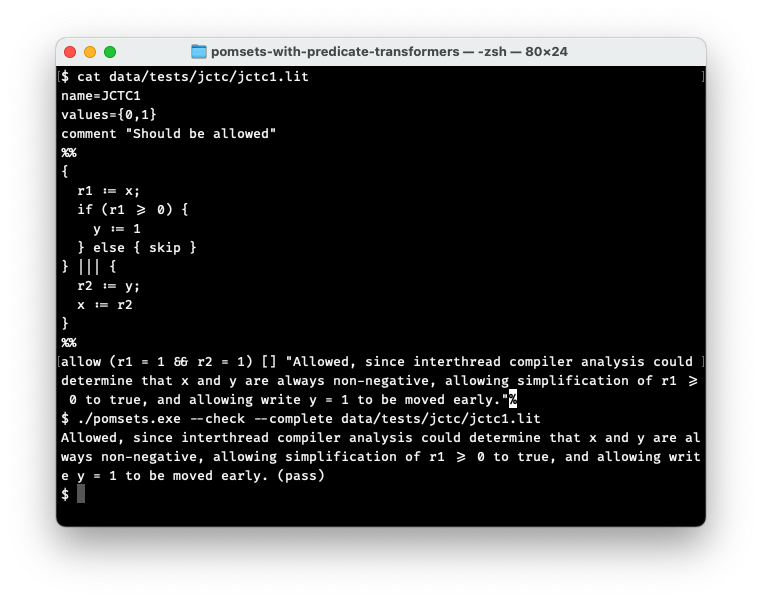
\includegraphics[width=0.75\textwidth]{tool.png}
  \Description{Image shows tool running on a Mac. Java Causality Test Case 1 is printed, followed by an invocation of the tool as {\tt ./pomsets.exe --check --complete data/tests/jctc/jctc1.lit}, which shows that the tool passes the assertion listed in the test.}
  \caption{\label{fig:tool} Example output of \PwTer, validating TC1~\cite{PughWebsite}.}
\end{center}
\end{figure}

\section{Refinements and Additional Features} %Case Analysis, Address Calculation, RMWs, Elimination}
\label{sec:additional}

In the paper so far, we have assumed that registers are assigned at most
once.  We have done this primarily for readability.  In the first subsection
below, we drop this assumption, instead using substitution to rename
registers.  We use the set
$\uRegs{\AllEvents}=\{\uReg{\aEv}\mid\aEv\in\AllEvents\}$.  By assumption
(\textsection\ref{sec:prelim}), these registers do not appear in programs:
$\aCmd[\bExp/\uReg{\aEv}]=\aCmd$.  The resulting semantics satisfies
redundant read elimination.

In this section we consider several mostly-orthogonal features: address
calculation, if-closure, fences, and read-modify-write operations.  Address
calculation and if-closure do have some interaction, and we spell out the
combined semantics in \textsection\ref{sec:semcaaddr}.

It is worth pointing out that address calculation and if-closure only affect
the semantics of read and write.  Fences introduce new trivial actions.
\RMW{}s require more infrastructure in order to ensure atomicity while
compiling to \armeight{}.

These extensions preserve all of the program transformation discussed thus
far, and apply equally to the various semantics we have discussed: \PwT{},
\PwTmca{1}, \PwTmca{2}, and \PwTc{}.  The results discussed in
\textsection\ref{sec:results} also apply equally, with the exception of
\RMW{}s: we have not proven \drfsc{} or \armeight lowering for \RMW{}s.


\subsection{Register Recycling and Redundant Read Elimination}
\label{sec:semreg}

\jmm{} Test Case 2 \citep{PughWebsite} states the following
execution should be allowed ``since redundant read elimination could result
in simplification of $\aReg{=}\bReg$ to true, allowing $\PW{y}{1}$ to be
moved early.''
\begin{gather*}
  \PR{x}{r}\SEMI
  \PR{x}{s}\SEMI
  \IF{r{=}s}\THEN \PW{y}{1}\FI
  \PAR
  \PW{x}{y}
  \\
  \hbox{\begin{tikzinline}[node distance=1.5em]
      \eventl{\bEv}{a1}{\DR{x}{1}}{}
      % \event{a2}{\DR{x}{1}}{right=of a1}
      \eventr{\aEv}{a3}{\DW{y}{1}}{right=of a1}
      % \po{a1}{a3}
      % \po[out=-20,in=-160]{a1}{a3}
      \event{b1}{\DR{y}{1}}{right=3em of a3}
      \event{b2}{\DW{x}{1}}{right=of b1}
      \rf{a3}{b1}
      \po{b1}{b2}
      % \rf[out=169,in=11]{b2}{a2}
      \rf[out=169,in=11]{b2}{a1}
    \end{tikzinline}}
\end{gather*}
This execution is not allowed by the semantics \reffig{fig:seq}: the precondition of
$\aEv$ in the independent case is
\begin{displaymath}
  \tag{$*$}\label{eq3}
  (1{=}r \lor x{=}r)\limplies (1{=}s \lor r{=}s)\limplies (r{=}s),
\end{displaymath}
which is equivalent to
\begin{math}
  (x{=}r)\limplies (1{=}s)\limplies (r{=}s),
\end{math}
which is not a tautology, and thus \reffig{fig:seq} requires order from
$\bEv$  to $\aEv$ in order to complete the pomset.

This execution is allowed, however, if we rename registers using a map from
event names to register names.  By using this renaming, coalesced events must
choose the same register name.  In the above example, the precondition of
$\aEv$ in the independent case becomes
\begin{displaymath}
  \tag{$**$}\label{eq4}
  (1{=}\uReg{\aEv} \lor x{=}\uReg{\aEv})\limplies (1{=}\uReg{\aEv} \lor \uReg{\aEv}{=}\uReg{\aEv})\limplies (\uReg{\aEv}{=}\uReg{\aEv}),
\end{displaymath}
which is a tautology.  In \eqref{eq4}, the first read resolves the
nondeterminism in both the first and the second read.  Given the choice of
event names, the outcome of the second read is predetermined!  In
\eqref{eq3}, the second read remains nondeterministic, even in the case that
the events are destined to coalesce.  

\begin{definition}
  Let $\semreg{}$ be defined as in \reffig{fig:seq}, changing \ref{read-tau}
  of $\sLOAD{}{}$:

  \noindent
  \begin{enumerate}[topsep=0pt,label=(\textsc{r}\arabic*),ref=\textsc{r}\arabic*]
    % \item \label{read-E}
    %   if $\bEv,\aEv\in\aEvs$ then $\bEv=\aEv$,
    % \item \label{read-lambda}
    %   $\labelingAct(\aEv) = \DR[\amode]{\aLoc}[\ascope]{\aVal}[\aThrd]$,
    %   \stepcounter{enumi}
    %   \stepcounter{enumi}
    \setcounter{enumi}{4}
  \item[] \labeltext[\textsc{r}4]{}{read-tau-reg}
    \begin{enumerate}[leftmargin=0pt]
    \item \label{read-tau-dep-reg}
      if $\aEv\in\aEvs$ and $\aEv\in\bEvs$ then
      \begin{math}
        \aTr{\bEvs}{\bForm} \riff
        \aVal{=}\uReg{\aEv}
        \limplies \bForm[\uReg{\aEv}/\aReg]
      \end{math},    
    \item \label{read-tau-ind-reg}
      if $\aEv\in\aEvs$ and $\aEv\notin\bEvs$ then
      \begin{math}
        \aTr{\bEvs}{\bForm} \riff
        \PBR{\aVal{=}\uReg{\aEv} \lor \aLoc{=}\uReg{\aEv}} \limplies
        \bForm[\uReg{\aEv}/\aReg],
      \end{math}
    \item \label{read-tau-empty-reg}
      if $\aEvs=\emptyset$ then $(\forall\bReg)$
      \begin{math}
        \aTr{\bEvs}{\bForm} \riff
        \bForm[\bReg/\aReg].
      \end{math}
    \end{enumerate}
  \end{enumerate}
  % \medskip
  % Similarly, let $\frf{\semreg{}}$ be defined as for
  % $\frf{\semrr{}}$ in \refdef{def:sem:frf}, with this definition of
  % $\sLOAD{}{}$.
\end{definition}


With this semantics, it is straightforward to see that redundant load
elimination is sound:
\begin{displaymath}
  \semreg{\PR[\amode]{\aLoc}{\aReg} \SEMI \PR[\amode]{\aLoc}{\bReg}} \supseteq 
  \semreg{\PR[\amode]{\aLoc}{\aReg} \SEMI \bReg  \GETS \aReg}
\end{displaymath}

As a further example, consider \cite[Fig.~5]{DBLP:conf/ecoop/SevcikA08},
referenced in \cite[\textsection6.4]{DBLP:conf/esop/PaviottiCPWOB20}.
Consider the case where the reads are merged, both seeing 1:
\begin{align*}
  \PR{y}{r}
  \SEMI
  \IF{r{=}1}\THEN \PR{y}{s} \SEMI \PW{x}{s}
  \ELSE \PW{x}{1}
  \FI
  &&
  \hbox{\begin{tikzinline}[node distance=1.5em]
      \event{a}{\DR{y}{1}}{}
      \event{b}{\aForm\mid\DW{x}{1}}{right=of a}
    \end{tikzinline}}
\end{align*}
In order to independent of both reads, we take the precondition $\aForm$ to be:
\begin{displaymath}
  \PBR{
    1{=}r\lor y{=}r
  }
  \limplies
  \SBR{
    r{=}1
    \land
    \PBRbig{
      \PBR{
        1{=}s\lor y{=}s
      }
      \limplies
      s{=}1
    }
  }
  \lor
  \SBR{
    r{\neq}1
  }
\end{displaymath}
Then collapsing $r$ and $s$ and substituting the initial value of $y$ (say $0$), we have a tautology:
\begin{displaymath}
  \PBR{
    1{=}r\lor 0{=}r
  }
  \limplies
  \SBR{
    r{=}1
    \land
    \PBRbig{
      \PBR{
        1{=}r\lor 0{=}r
      }
      \limplies
      r{=}1
    }
  }
  \lor
  \SBR{
    r{\neq}1
  }
\end{displaymath}


\subsection{Address Calculation}
\label{sec:addr}

Inevitably, address calculation complicates the definitions of $\sSTORE{}{}$ and $\sLOAD{}{}$.
\begin{definition}
  \label{def:semaddr}
  Let $\semaddr{}$ be defined as in \reffig{fig:seq}, changing $\sSTORE{}{}$ and $\sLOAD{}{}$:

  \noindent
  If $\aPS \in \sSTORE[\amode]{\cExp}[\ascope]{\aExp}[\aThrd]$ then
  $(\exists\cVal\in\Val)$
  $(\exists\aVal\in\Val)$
  \begin{multicols}{2}
    \begin{enumerate}[topsep=0pt,label=(\textsc{w}\arabic*),ref=\textsc{w}\arabic*]
    \item \label{write-E-addr}
      if $\fcard{\aEvs}\leq1$,
    \item \label{write-lambda-addr}
      $\labelingAct(\aEv) = \DW[\amode]{\REF{\cVal}}[\ascope]{\aVal}[\aThrd]$,
    \item \label{write-kappa-addr}
      \begin{math}
        \labelingForm(\aEv) \riff
        \cExp{=}\cVal
        \land \aExp{=}\aVal
      \end{math},      
      \stepcounter{enumi}
    \item[] \labeltext[\textsc{w}4]{}{write-tau-addr}
      \begin{enumerate}[leftmargin=0pt]
      \item \label{write-tau-dep-addr}
        if $\aEvs\neq\emptyset$ then 
        \makebox[0pt][l]{\begin{math}
          \aTr{\bEvs}{\bForm} \riff 
          (\cExp{=}\cVal)
          \limplies 
          \bForm[\aExp/\REF{\cVal}][\aExp{=}\aVal/\Q{\REF{\cVal}}]
        \end{math},}
      \item \label{write-tau-empty-addr}
        if $\aEvs=\emptyset$ then
        \makebox[0pt][l]{\begin{math}
          (\forall\dVal)
        \end{math}        
        \begin{math}
          \aTr{\bEvs}{\bForm} \riff 
          (\cExp{=}\dVal)
          \limplies 
          \bForm
          [\aExp/\REF{\dVal}][\FALSE/\Q{\REF{\dVal}}],
        \end{math}}
      \end{enumerate}
      \columnbreak
      \stepcounter{enumi}
    \item[] \labeltext[\textsc{w}5]{}{write-term-addr}
      \begin{enumerate}[leftmargin=0pt]
      \item \label{write-term-nonempty-addr}
        if $\aEvs\neq\emptyset$ then $\aTerm \riff \cExp{=}\cVal \land \aExp{=}\aVal$,
      \item \label{write-term-empty-addr}
        if $\aEvs=\emptyset$ then $\aTerm \riff \FALSE$.
      \end{enumerate}
    \end{enumerate}
  \end{multicols}

  \medskip
  \noindent
  If $\aPS \in \sLOAD[\amode]{\aReg}[\ascope]{\cExp}[\aThrd]$ then
  $(\exists\cVal\in\Val)$
  $(\exists\aVal\in\Val)$
  \begin{multicols}{2}
    \begin{enumerate}[topsep=0pt,label=(\textsc{r}\arabic*),ref=\textsc{r}\arabic*]
    \item \label{read-E-addr}
      if $\fcard{\aEvs}\leq1$,
    \item \label{read-lambda-addr}
      $\labelingAct(\aEv) = \DR[\amode]{\REF{\cVal}}[\ascope]{\aVal}[\aThrd]$
    \item \label{read-kappa-addr}
      \begin{math}
        \labelingForm(\aEv) 
        \riff
        \cExp{=}\cVal
        \land \Q{\REF{\cVal}}
      \end{math},
      \stepcounter{enumi}
    \item[] \labeltext[\textsc{r}4]{}{read-tau-addr}
      \begin{enumerate}[leftmargin=0pt]
      \item \label{read-tau-dep-addr}
        if $\aEv\in\aEvs$ and $\aEv\in\bEvs$ then
        % \begin{math}
        %   (\forall\aEv\in\aEvs\cap\bEvs)
        % \end{math}
        \makebox[0pt][l]{\begin{math}
            \aTr{\bEvs}{\bForm} \riff
            (\cExp{=}\cVal\limplies\aVal{=}\uReg{\aEv})
            \limplies \bForm[\uReg{\aEv}/\aReg]
          \end{math},}
      \item \label{read-tau-ind-addr}
        if $\aEv\in\aEvs$ and $\aEv\not\in\bEvs$ then
        % \begin{math}
        %   (\forall\aEv\in\aEvs\setminus\bEvs)
        % \end{math}
        \makebox[0pt][l]{\begin{math}
            \aTr{\bEvs}{\bForm} \riff
            \PBR{(\cExp{=}\cVal\limplies\aVal{=}\uReg{\aEv}) \lor (\cExp{=}\cVal\limplies\REF{\cVal}{=}\uReg{\aEv})}
            \limplies
            \bForm[\uReg{\aEv}/\aReg]
          \end{math},}
        \columnbreak
      \item \label{read-tau-empty-addr}
        if $\aEvs=\emptyset$ then 
        \begin{math}
          (\forall\bReg)
        \end{math}
        \begin{math}
          \aTr{\bEvs}{\bForm} \riff 
          \bForm[\bReg/\aReg],
        \end{math}  
      \end{enumerate}  
      \stepcounter{enumi}
    \item[] \labeltext[\textsc{r}5]{}{read-term-addr}
      \begin{enumerate}[leftmargin=0pt]
      \item \label{read-term-nonempty-addr}
        if $\aEvs\neq\emptyset$ or $\amode\lemode\mRLX$ then $\aTerm \riff \TRUE$. 
      \item \label{read-term-empty-addr}
        if $\aEvs=\emptyset$ and $\amode\gemode\mACQ$ then $\aTerm \riff \FALSE$. 
      \end{enumerate}      
    % \item \label{read-term-addr}
    %   if $\aEvs=\emptyset$ and $\amode\neq\mRLX$ then $\aTerm \riff \FALSE$. 
    \end{enumerate}
  \end{multicols}
\end{definition}

The combination of read-read independency (\textsection\ref{sec:read-read}) and address
calculation is somewhat delicate.  
% , in
% \ref{read-tau-dep-addr}.  The subsection of \textsection\ref{sec:diff} on
% \ref{xCausal} discusses this example using the semantics of \jjr{}.
Consider the following program, from \cite[\textsection5]{DBLP:journals/pacmpl/JagadeesanJR20}, where initially $x=0$, $y=0$, $\REF{0}=0$,
$\REF{1}=2$, and $\REF{2}=1$.  It should only be possible to read $0$,
disallowing the attempted execution below:
\begin{gather*}
  \begin{gathered}
    \PR{y}{r}\SEMI \PR{\REF{r}}{s}\SEMI \PW{x}{s}
    \PAR
    \PR{x}{r}\SEMI \PR{\REF{r}}{s}\SEMI \PW{y}{s}
    \\[-1ex]
    \hbox{\begin{tikzinline}[node distance=1.5em]
        \event{a1}{\DR{y}{2}}{}
        \event{a2}{\DR{\REF{2}}{1}}{right=of a1}
        \event{a3}{\DW{x}{1}}{right=of a2}
        \po{a2}{a3}
        \po[out=15,in=165]{a1}{a3}
        \event{b1}{\DR{x}{1}}{right=3em of a3}
        \event{b2}{\DR{\REF{1}}{2}}{right=of b1}
        \event{b3}{\DW{y}{2}}{right=of b2}
        \po{b2}{b3}
        \po[out=15,in=165]{b1}{b3}
        \rf[out=-170,in=-10]{b3}{a1}
        \rf{a3}{b1}
      \end{tikzinline}}
  \end{gathered}
\end{gather*}
This execution would become possible, however, if we were to replace
$(\cExp{=}\cVal\limplies\aVal{=}\uReg{\aEv})$ by $(\aVal{=}\uReg{\aEv})$ in
\ref{read-tau-dep-addr}.  In this case, $\DRP{y}{2}$ would not necessarily be dependency
ordered before $\DWP{x}{1}$.
% % 
% In isolation, the precondition of $\DWP{x}{1}$ is $(s=1)$.  Using the erroneous
% definition of \ref{read-tau-dep-addr}, the precondition becomes $(1{=}s)\limplies (s=1)$

% Looking at the left thread:
% \begin{align*}
%   \begin{gathered}[t]
%     \PR{y}{r}
%     \\
%     \hbox{\begin{tikzinline}[node distance=.5em and 1.5em]
%       \event{a}{\DR{y}{2}}{}
%       \xform{xi}{(2{=}r\lor\RW)\limplies\bForm}{above=of a}
%       \xform{xd}{2{=}r\limplies\bForm}{below=of a}
%       \xo[xright]{a}{xd}
%     \end{tikzinline}}
%   \end{gathered}
%   &&
%   \begin{gathered}[t]
%     \PR{\REF{r}}{s}
%     \\
%     \hbox{\begin{tikzinline}[node distance=.5em and 1.5em]
%       \event{b}{r\EQ2\mid\DR{\REF{2}}{1}}{}
%       \xform{xd}{(r\EQ2\limplies 1\EQ s) \limplies\bForm}{below=of b}
%       \xform{xi}{((r\EQ2\limplies 1\EQ s)\lor\RW) \limplies\bForm}{above=of b}
%       \xo[xright]{b}{xd}
%     \end{tikzinline}}
%   \end{gathered}
%   &&
%   \begin{gathered}[t]
%     \PW{x}{s}
%     \\
%     \hbox{\begin{tikzinline}[node distance=.5em and 1.5em]
%       \event{b}{s\EQ1\mid\DW{x}{1}}{}
%       \xform{xd}{\bForm}{below=of b}
%       \xform{xi}{\bForm}{above=of b}
%       \xo[out=-30]{b}{xd}
%     \end{tikzinline}}
%   \end{gathered}
% \end{align*}
% Composing, we have:
% \begin{gather*}
%   \begin{gathered}
%     \PR{y}{r}\SEMI \PR{\REF{r}}{s}\SEMI \PW{x}{s}
%     \\
%     \hbox{\begin{tikzinline}[node distance=.5em and 1.5em]
%       \event{a1}{\DR{y}{2}}{}
%       \event{a2}{(2{=}r\lor\RW)\limplies r\EQ2\mid\DR{\REF{2}}{1}}{right=of a1}
%       \event{a3}{(2{=}r\lor\RW)\limplies (r\EQ2\limplies 1\EQ s)
%       \limplies s\EQ1\mid\DW{x}{1}}{below right=.5em and -8em of a2}
%       \po{a2}{a3}
%     \end{tikzinline}}
%   \end{gathered}
% \end{gather*}  
% Substituting for $\RW$:
% \begin{gather*}
%   \begin{gathered}
%     %     \PR{y}{r}\SEMI \PR{\REF{r}}{s}\SEMI \PW{x}{s}
%     %     \\
%     \hbox{\begin{tikzinline}[node distance=.5em and 1.5em]
%       \event{a1}{\DR{y}{2}}{}
%       \event{a2}{(2{=}r\lor\FALSE)\limplies r\EQ2\mid\DR{\REF{2}}{1}}{right=of a1}
%       \event{a3}{(2{=}r\lor\TRUE)\limplies (r\EQ2\limplies 1\EQ s)
%       \limplies s\EQ1\mid\DW{x}{1}}{below right=.5em and -8em of a2}
%       \po{a2}{a3}
%     \end{tikzinline}}
%   \end{gathered}
% \end{gather*}
% Which is:
% \begin{gather*}
%   \begin{gathered}
%     %     \PR{y}{r}\SEMI \PR{\REF{r}}{s}\SEMI \PW{x}{s}
%     %     \\
%     \hbox{\begin{tikzinline}[node distance=.5em and 1.5em]
%       \event{a1}{\DR{y}{2}}{}
%       \event{a2}{2{=}r\limplies r\EQ2\mid\DR{\REF{2}}{1}}{right=of a1}
%       \event{a3}{(r\EQ2\limplies 1\EQ s)
%       \limplies s\EQ1\mid\DW{x}{1}}{below right=.5em and -8em of a2}
%       \po{a2}{a3}
%     \end{tikzinline}}
%   \end{gathered}
% \end{gather*}
% The precondition of $\DRP{\REF{2}}{1}$ is a tautology, but the precondition
% of $\DWP{x}{1}$ is not.  This forces a dependency:
% \begin{gather*}
%   \begin{gathered}
%     \PR{y}{r}\SEMI \PR{\REF{r}}{s}\SEMI \PW{x}{s}
%     \\
%     \hbox{\begin{tikzinline}[node distance=.5em and 1.5em]
%       \event{a1}{\DR{y}{2}}{}
%       \event{a2}{2{=}r\limplies r\EQ2\mid\DR{\REF{2}}{1}}{right=of a1}
%       \event{a3}{2{=}r\limplies (r\EQ2\limplies 1\EQ s)
%       \limplies s\EQ1\mid\DW{x}{1}}{below right=.5em and -5em of a2}
%       \po[out=-20,in=180]{a1}{a3}
%       \po{a2}{a3}
%     \end{tikzinline}}
%   \end{gathered}
% \end{gather*}
% All the preconditions are now tautologies.

\subsection{Fences and Read-Modify-Write Operations}
\label{sec:fences}
\label{sec:rmw}

The semantics of fences is straightforward.
Let
\begin{math}
  \sembase{\PF[\ascope]{\fmode}} = \sFENCE[\ascope]{\fmode}[\aThrd],
\end{math}
where
if $\aPS \in \sFENCE[\ascope]{\amode}[\aThrd]$ then
% $(\exists\aLocs\subseteq\Loc)$
% $(\exists\bmode\in\{\amode,\mRLX\})$
\begin{multicols}{3}
  \begin{enumerate}[topsep=0pt,label=(\textsc{f}\arabic*),ref=\textsc{f}\arabic*]
  \item \label{fence-E}
    % $\aEvs\neq\emptyset$ and
    % if $\bEv,\aEv\in\aEvs$ then $\bEv=\aEv$,
    $\fcard{\aEvs}\leq 1$,
  \item \label{fence-lambda}
    $\labelingAct(\aEv) = \DF[\ascope]{\amode}[\aThrd]$,
  \item \label{fence-kappa}
    $\labelingForm(\aEv) \riff \TRUE$,
  \item \label{fence-tau}
    $\aTr{\bEvs}{\bForm} \riff \bForm$,
    \stepcounter{enumi}      
  \item[] \labeltext[\textsc{f}5]{}{fence-term}
    \begin{enumerate}[leftmargin=0pt]
    \item \label{fence-term-nonempty}
      if $\aEvs\neq\emptyset$ then $\aTerm \riff \TRUE$,
    \item \label{fence-term-empty}
      if $\aEvs=\emptyset$ then $\aTerm \riff \FALSE$.
    \end{enumerate}
    % \item \label{fence-term}
    %   if $\aEvs=\emptyset$ then $\aTerm \riff \FALSE$.
  \end{enumerate}
\end{multicols}
This semantics is identical to that of
\cite{DBLP:journals/pacmpl/JagadeesanJR20}; see there for examples.

% \subsection{}

%We give the semantics of \RMW{}s without address calculation or if-closure.

% From the data model, we require an additional binary relation over
% $\Act\times\Act$: $\roverlapsdef$.  For the actions in this paper, we say
% $\aAct \roverlapsdef \bAct$ if they access the same location.

\RMW{} operations are more complex.  To support \RMW{}s, we add a relation
${\xrmw}\subseteq\aEvs\times\aEvs$ that relates the read of a successful
\RMW{} to the succeeding write.
% Let two actions \emph{overlap} if they access the same location.
% \begin{enumerate}
% \item
%   ${\rrmw} \subseteq {\le}$ is a relation capturing
%   \emph{read-modify-write atomicity}, such that for any $\cEv$, $\bEv$, $\aEv\in\aEvs$,
%   where $\labeling(\cEv)$ and
%   $\labeling(\bEv)$ access the same location:
%   \begin{itemize}
%   \item if $\bEv \xrmw \aEv$ and $\cEv\le \aEv$ then $\cEv\le \bEv$,
%   \item if $\bEv \xrmw \aEv$ and $\bEv\le \cEv$ then $\aEv\le \cEv$.
%   \end{itemize}
% \end{enumerate}

\begin{definition}
  Extend the definition of a pomset as follows. % where two actions \emph{overlap} if they access the same location:
  \begin{enumerate}[,label=(\textsc{m}\arabic*),ref=\textsc{m}\arabic*]
    \setcounter{enumi}{9}
  \item \label{pom-rmw}
    ${\rrmw} : \aEvs\fun\aEvs$ is a partial function capturing
    read-modify-write \emph{atomicity}, such that
    \begin{enumerate}
    \item \label{pom-rmw-block}
      if $\bEv\xrmw\aEv$ then $\labeling(\aEv) \rblocks \labeling(\bEv)$,
    \item \label{pom-rmw-le}
      if $\bEv\xrmw\aEv$ then $\bEv \le \aEv$,    
    \item \label{pom-rmw-atomic}
      if $\labeling(\cEv) \roverlaps \labeling(\bEv)$ then
      \begin{enumerate}        
      \item \label{pom-rmw-atomic1}
        if $\bEv \xrmw \aEv$ then
        $\cEv\le \aEv$ implies $\cEv\le \bEv$,
      \item \label{pom-rmw-atomic2}
        if $\bEv \xrmw \aEv$ then
        $\bEv\le \cEv$ implies $\aEv\le \cEv$.
      \end{enumerate}
    \end{enumerate}
  \end{enumerate}

  Extend the definition of $\sSEMI{}{}$ and $\sIF{}{}{}$ to include:
  \begin{enumerate}
  \item[(\textsc{s}10)] (\textsc{i}10)\; % (\textsc{p}10)\; 
    ${\rrmw}=\PBR{{\rrmw_1}\cup{\rrmw_2}}$,
  \end{enumerate}
\end{definition}

To define specific operations, we extend the syntax:
\begin{align*}
  \aCmd
  \BNFDEF& \cdots 
  \BNFSEP \PCAS[\amode][\bmode]{\REF{\cExp}}[\ascope]{\aReg}{\aExp}{\bExp}
  \BNFSEP \PFADD[\amode][\bmode]{\REF{\cExp}}[\ascope]{\aReg}{\aExp}
  \BNFSEP \PEXCHG[\amode][\bmode]{\REF{\cExp}}[\ascope]{\aReg}{\aExp}
\end{align*}
We require that $\aReg$ does not occur in $\cExp$.  The corresponding semantic functions are as follows.
\begin{definition}
  Let $\sLOADP{}{}$ be defined as for $\sLOAD{}{}$, adding the constraint:
  \begin{itemize}
  \item[{\labeltext[\textsc{r}4d]{(\textsc{r}4d)}{read-tau-rmw}}]
    if $(\aEvs\cap\bEvs)=\emptyset$ then
    \begin{math}
      \aTr{\bEvs}{\bForm} \rimplies
      \bForm.
    \end{math}
  \end{itemize}
  If $\aPS\in\mathit{FADD}(\aReg,\cExp,\aExp,\amode,\bmode)$ then
  $(\exists \aPS_1\in\sSEMI{\sLOADP[\amode]{\aReg}{\cExp}}{\sSTORE[\bmode]{\cExp}{\aReg{+}\aExp}})$
  \begin{enumerate}[topsep=0pt,label=(\textsc{u}\arabic*),ref=\textsc{u}\arabic*]
  \item if $\labeling_1(\aEv)$ is a write then there is a read $\labeling_1(\bEv)$ such that 
    $\labelingForm(\aEv)\rimplies\labelingForm(\bEv)$ and
    $\bEv\xrmw\aEv$.
  \end{enumerate}
  If $\aPS\in\mathit{EXCHG}(\aReg,\cExp,\aExp,\amode,\bmode)$ then
  $(\exists \aPS_1\in\sSEMI{\sLOADP[\amode]{\aReg}{\cExp}}{\sSTORE[\bmode]{\cExp}{\aExp}})$
  \begin{enumerate}[topsep=0pt,label=(\textsc{u}\arabic*),ref=\textsc{u}\arabic*]
  \item if $\labeling_1(\aEv)$ is a write then there is a read $\labeling_1(\bEv)$ such that 
    $\labelingForm(\aEv)\rimplies\labelingForm(\bEv)$ and
    $\bEv\xrmw\aEv$.
  \end{enumerate}
  If $\aPS\in\mathit{CAS}(\aReg,\cExp,\aExp,\bExp,\amode,\bmode)$ then
  $(\exists \aPS_1\in\sSEMI{\sLOADP[\amode]{\aReg}{\cExp}}{\sIF{\aReg{=}\aExp}\sTHEN\sSTORE[\bmode]{\cExp}{\bExp}\sELSE\sSKIP\sFI})$
  \begin{enumerate}[topsep=0pt,label=(\textsc{u}\arabic*),ref=\textsc{u}\arabic*]
  \item if $\labeling_1(\aEv)$ is a write then there is a read $\labeling_1(\bEv)$ such that 
    $\labelingForm(\aEv)\rimplies\labelingForm(\bEv)$ and
    $\bEv\xrmw\aEv$.
  \end{enumerate}
\end{definition}
  % If $\aPS\in\mathit{FADD}(\aReg,\aLoc,\aExp,\amode_1,\amode_2)$ then
  % $(\exists \aPS_1\in\sSEMI{\sLOADP[\amode_1]{\aReg}{\aLoc}}{\sSTORE[\amode_2]{\aLoc}{\aReg{+}\aExp}})$
  % \begin{enumerate}[topsep=0pt,label=(\textsc{u}\arabic*),ref=\textsc{u}\arabic*]
  % \item if $\labeling_1(\aEv)$ is a write then there is a read $\labeling_1(\bEv)$ such that 
  %   $\labelingForm(\aEv)\rimplies\labelingForm(\bEv)$ and
  %   $\bEv\xrmw\aEv$.
  %   % \item if $\labeling_1(\bEv)$ is a read, then there is a write $\labeling_1(\aEv)$ such that 
  %   %   $\labelingForm(\bEv)\rimplies\labelingForm(\aEv)$ and 
  %   %   $\bEv\xrmw\aEv$.
  % \end{enumerate}
  % If $\aPS\in\mathit{EXCHG}(\aReg,\aLoc,\aExp,\amode_1,\amode_2)$ then
  % $(\exists \aPS_1\in\sSEMI{\sLOADP[\amode_1]{\aReg}{\aLoc}}{\sSTORE[\amode_2]{\aLoc}{\aExp}})$
  % \begin{enumerate}[topsep=0pt,label=(\textsc{u}\arabic*),ref=\textsc{u}\arabic*]
  % \item if $\labeling_1(\aEv)$ is a write then there is a read $\labeling_1(\bEv)$ such that 
  %   $\labelingForm(\aEv)\rimplies\labelingForm(\bEv)$ and
  %   $\bEv\xrmw\aEv$.
  %   % \item if $\labeling_1(\bEv)$ is a read, then there is a write $\labeling_1(\aEv)$ such that 
  %   %   $\labelingForm(\bEv)\rimplies\labelingForm(\aEv)$ and 
  %   %   $\bEv\xrmw\aEv$.
  % \end{enumerate}
  % If $\aPS\in\mathit{CAS}(\aReg,\aLoc,\aExp,\bExp,\amode_1,\amode_2)$ then
  % $(\exists \aPS_1\in\sSEMI{\sLOADP[\amode_1]{\aReg}{\aLoc}}{\sIF{\aReg{=}\aExp}\sTHEN\sSTORE[\amode_2]{\aLoc}{\bExp}\sELSE\sSKIP\sFI})$
  % \begin{enumerate}[topsep=0pt,label=(\textsc{u}\arabic*),ref=\textsc{u}\arabic*]
  % \item if $\labeling_1(\aEv)$ is a write then there is a read $\labeling_1(\bEv)$ such that 
  %   $\labelingForm(\aEv)\rimplies\labelingForm(\bEv)$ and
  %   $\bEv\xrmw\aEv$.
  %   % \item if $\labeling_1(\bEv)$ is a read, then either
  %   %   \begin{enumerate}
  %   %   \item there is a write $\labeling_1(\aEv)$ such that $\labelingForm(\bEv)\rimplies\labelingForm(\aEv)$ and $\bEv\xrmw\aEv$, or
  %   %   \item 
  %   %   \end{enumerate}
  % \end{enumerate}
  % \begin{multicols}{2}
  %   \begin{enumerate}[topsep=0pt,label=(\textsc{u}\arabic*),ref=\textsc{u}\arabic*]
  %   \item if $\labeling_1(\aEv)$ is a write, then $(\exists\bEv)$ such that
  %     \begin{enumerate}
  %     \item $\labeling_1(\aEv)\rblocks \labeling_1(\bEv)$,
  %     \item $\bEv\xrmw\aEv$,
  %     \end{enumerate}
  %     \columnbreak
  %   \item if $\labeling_1(\bEv)$ is a read, then $(\exists\aEv)$ such that
  %     \begin{enumerate}
  %     \item $\labeling_1(\aEv)\rblocks \labeling_1(\bEv)$,
  %     \item $\bEv\xrmw\aEv$,
  %     \item
  %       if $(\aEvs\cap\bEvs)=\emptyset$ then
  %       \begin{math}
  %         \aTr{\bEvs}{\bForm} \rimplies \bForm[\aExp/\aLoc].
  %       \end{math}
  %     \end{enumerate}
  %   \end{enumerate}
  % \end{multicols}

This definition ensures atomicity and supports lowering to Arm load/store
exclusive operations.  See \cite{DBLP:journals/pacmpl/JagadeesanJR20} for examples.

One subtlety of the definition is that we use $\sLOADP{}{}$ rather than
$\sLOAD{}{}$.  Thus, for \RMW{} operations, the independent case for a read
is the same as the empty case.  To see why this should be, consider the
relaxed variant of the \textsc{cdrf} example from
\cite{DBLP:conf/pldi/LeeCPCHLV20}, using $\sLOAD{}{}$ rather than $\sLOADP{}{}$.
\begin{gather*}
  \begin{gathered}
    \PW{x}{0}\SEMI
    \begin{aligned}[t]
      (&\PFADD[\mRLX][\mRLX]{x}{r}{1}\SEMI \IF{\BANG r}\THEN \IF{y}\THEN \PW{x}{0} \FI \FI \;\;\PAR
      \\&
      \PFADD[\mRLX][\mRLX]{x}{r}{1}\SEMI \IF{\BANG r}\THEN \PW{y}{1} \FI)
    \end{aligned}
    \\
    \hbox{\begin{tikzinline}[node distance=1.5em]
        \event{i}{\DW{x}{0}}{}
        \event{b0}{\DR{x}{0}}{right=3em of i}
        \event{b0b}{\DW{x}{1}}{right=of b0}
        \event{b1}{\DR{y}{1}}{right=of b0b}
        \event{b2}{\DW{x}{0}}{right=of b1}
        \event{a1}{\DR{x}{0}}{right=3em of b2}
        \event{a1b}{\DW{x}{1}}{right=of a1}
        \event{a2}{\DW{y}{1}}{right=of a1b}
        \rmw{a1}{a1b}
        \rmw{b0}{b0b}
        \rf{i}{b0}
        \rf[out=-165,in=-12]{a2}{b1}
        \wki[out=20,in=160]{b0b}{b2}
        % \sync{a1}{a2}
        % \sync{b0}{b1}
        \po{b1}{b2}
        \rf{b2}{a1}
      \end{tikzinline}}
  \end{gathered}
\end{gather*}
A write should only be visible to one $\PFADD{}{}{}$ instruction, but here
the write of $0$ is visible to two.  This is allowed because no order is
required from $\DRP{x}{0}$ to $\DWP{y}{1}$ in the last thread.  To see why,
consider the independent transformers of the last thread and initializer:
\begin{align*}
  \begin{gathered}[t]
    \PW{x}{0}
    \\
    \hbox{\begin{tikzinline}[node distance=.5em]
        \event{a}{\DW{x}{0}}{}      
        \xform{xi}{\bForm[0/x]}{left=of a}
      \end{tikzinline}}    
  \end{gathered}
  &&
  \begin{gathered}[t]
    \smash{\FADD^{\mRLX,\mRLX}(x,1)}
    \\
    \hbox{\begin{tikzinline}[node distance=1.5em]
        \event{a0}{\DR{x}{0}}{}
        %\node(a)[right=of a0]{};
        \event{a1}{\DW{x}{1}}{right=of a0}
        \rmw{a0}{a1}
        \xform{xi}{(0{=}r\lor x{=}r)\limplies\bForm[1/x]}{left=.5em of a0}
      \end{tikzinline}}    
  \end{gathered}
  &&
  \begin{gathered}[t]
    \IF{\BANG r}\THEN \PW{y}{1} \FI
    \\
    \hbox{\begin{tikzinline}[node distance=.5em]
        \event{a2}{r{=}0\mid\DW{y}{1}}{}      
        \xform{xi}{\bForm[1/y]}{left=of a2}
      \end{tikzinline}}    
  \end{gathered}
\end{align*}
After sequencing, the precondition of $\DWP{y}{1}$ is a tautology:
$(0{=}r\lor 0{=}r)\limplies r{=}0$.

By including \ref{read-tau-rmw}, $\sLOADP{}{}$ constrains the independent
predicate transformer of the $\PFADD{}{}{}$:
\begin{align*}
  \begin{gathered}[t]
    \PW{x}{0}
    \\
    \hbox{\begin{tikzinline}[node distance=.5em]
        \event{a}{\DW{x}{0}}{}      
        \xform{xi}{\bForm[0/x]}{left=of a}
      \end{tikzinline}}    
  \end{gathered}
  &&
  \begin{gathered}[t]
    \smash{\FADD^{\mRLX,\mRLX}(x,1)}
    \\
    \hbox{\begin{tikzinline}[node distance=1.5em]
        \event{a0}{\DR{x}{0}}{}
        %\node(a)[right=of a0]{};
        \event{a1}{\DW{x}{1}}{right=of a0}
        \rmw{a0}{a1}
        \xform{xi}{\bForm[1/x]}{left=.5em of a0}
      \end{tikzinline}}    
  \end{gathered}
  &&
  \begin{gathered}[t]
    \IF{\BANG r}\THEN \PW{y}{1} \FI
    \\
    \hbox{\begin{tikzinline}[node distance=.5em]
        \event{a2}{r{=}0\mid\DW{y}{1}}{}      
        \xform{xi}{\bForm[1/y]}{left=of a2}
      \end{tikzinline}}    
  \end{gathered}
\end{align*}
After sequencing, the precondition of $\DWP{y}{1}$ is $r{=}0$, which is
\emph{not} a tautology.  This forces any top-level pomset to include
dependency order from $\DRP{x}{0}$ to $\DWP{y}{1}$.

% Here, local invariant reasoning is using the initializing write to $x$ to
% justify the independence of the write to $y$.  But this write is made
% unavailable by the first thread's successful \RMW{}.


\begin{comment}
  For case analysis of RMWs, we can use a general purpose expansion operator:

  \begin{definition}
    \noindent
    If $\aPS \in \sEXPAND\aPSS$ then
    $(\exists\aPS_1,\ldots,\aPS_n\in\aPSS)$
    $(\exists\cForm_1,\ldots,\cForm_n\in\Formulae)$
    % \\ let $\aPS_\aEv=\aPS_i$ if $\aEv\in\aEvs_i$ and $\cForm_\aEv=\cForm_i$ if $\aEv\in\aEvs_i$
    \begin{multicols}{2}
      \begin{enumerate}[topsep=0pt,label=(\textsc{e}\arabic*),ref=\textsc{e}\arabic*]
      \item[] \label{ca-psi}
        \begin{enumerate}[leftmargin=0pt]
        \item if $\cForm_i\land\cForm_j$ is satisfiable then $i=j$,        
        \item $\bigvee_i\cForm_i\riff\TRUE$,        
        \end{enumerate}
        \stepcounter{enumi}
      \item[] \label{ca-E}
        \begin{enumerate}[leftmargin=0pt]
        \item if $\aEvs_i\cap\aEvs_j\neq\emptyset$ then $i=j$,
        \item $\aEvs=\bigcup_i\aEvs_i$, %(\aEvs_1\cup\cdots\cup\aEvs_n)$,
          % \item if $\cForm_\aEv\land\cForm_\bEv$ is satisfiable then
          %   $(\exists i)$ $\aEv,\bEv\in\aEvs_i$,
        \end{enumerate}
      \item \label{ca-lambda}
        ${\labeling}=\bigcup_i{\labeling_i}$,%\PBR{{\labeling_1}\cup\cdots \cup {\labeling_n}}$,       
      \item \label{ca-kappa}
        \begin{math}
          \labelingForm(\aEv) \riff
          \cForm_\aEv\land \labelingForm_\aEv(\aEv)
        \end{math},
      \item \label{ca-tau}
        \begin{math}
          \aTr{\bEvs}{\bForm} \riff 
          \bigvee_i (\cForm_i\land \aTr[i]{\bEvs}{\bForm})
        \end{math},
      \item \label{ca-term}
        $\aTerm \riff \bigvee_i (\cForm_i\land \aTerm[i])$,
      \item ${\rrfx}=\bigcup_i{\rrfx_i}$,
      \item ${\le}=\bigcup_i{\le_i}$.
      \end{enumerate}
    \end{multicols}
  \end{definition}
\end{comment}


\subsection{If-Closure}
\label{sec:semca}

In order to model sequential composition, we must allow inconsistent
predicates in a single pomset, unlike \PwP{}
\cite{DBLP:journals/pacmpl/JagadeesanJR20}.  For example, if
$\aCmd=(\PW{x}{1})$, then the semantics \reffig{fig:seq} does \emph{not} allow:
\begin{gather*}
  \IF{\aExp}\THEN\PW{x}{1}\FI
  \SEMI
  \aCmd
  \SEMI
  \IF{\lnot\aExp}\THEN\PW{x}{1}\FI
  \\
  \hbox{\begin{tikzinline}[node distance=1.5em]
      \event{a}{\DW{x}{1}}{}
      \event{b}{\DW{x}{1}}{right=of a}
      \wki{a}{b}
    \end{tikzinline}}
\end{gather*}
However, if
$\aCmd=(\IF{\lnot\aExp}\THEN\PW{x}{1}\FI\SEMI\IF{\aExp}\THEN\PW{x}{1}\FI)$,
then it %\refdef{def:pomsets-trans}
\emph{does} allow the execution.  Looking at the initial program:
\begin{align*}
  \begin{gathered}
    \IF{\aExp}\THEN\PW{x}{1}\FI
    \\
    \hbox{\begin{tikzinline}[node distance=1em]
        \event{a}{\aExp\mid\DW{x}{1}}{}
      \end{tikzinline}}
  \end{gathered}
  &&
  \begin{gathered}
    \PW{x}{1}
    \\
    \hbox{\begin{tikzinline}[node distance=1em]
        \event{a}{\DW{x}{1}}{}
      \end{tikzinline}}
  \end{gathered}
  &&
  \begin{gathered}
    \IF{\lnot\aExp}\THEN\PW{x}{1}\FI
    \\
    \hbox{\begin{tikzinline}[node distance=1em]
        \event{a}{\lnot\aExp\mid\DW{x}{1}}{}
      \end{tikzinline}}
  \end{gathered}
\end{align*}
\noindent
The difficulty is that the middle action can coalesce either with the right
action, or the left, but not both.  Thus, we are stuck with some
non-tautological precondition.  Our solution is to allow a pomset to
contain many events for a single action, as long as the events have
disjoint preconditions.

\refdef{def:semca} allows the execution, by splitting the middle command:
\begin{align*}
  \begin{gathered}
    \IF{\aExp}\THEN\PW{x}{1}\FI
    \\
    \hbox{\begin{tikzinline}[node distance=1em]
        \eventl{d}{a}{\aExp\mid\DW{x}{1}}{}
      \end{tikzinline}}
  \end{gathered}
  &&
  \begin{gathered}
    \PW{x}{1}
    \\
    \hbox{\begin{tikzinline}[node distance=1.5em]
        \eventl{d}{a}{\lnot\aExp\mid\DW{x}{1}}{}
        \eventl{e}{b}{\aExp\mid\DW{x}{1}}{right=of a}
      \end{tikzinline}}
  \end{gathered}
  &&
  \begin{gathered}
    \IF{\lnot\aExp}\THEN\PW{x}{1}\FI
    \\
    \hbox{\begin{tikzinline}[node distance=1em]
        \eventl{e}{a}{\lnot\aExp\mid\DW{x}{1}}{}
      \end{tikzinline}}
  \end{gathered}
\end{align*}
Coalescing events gives the desired result.


This is not simply a theoretical question; it is observable.  For example,
the semantics of \reffig{fig:seq} does not allow the following, since it must add order in the
first thread from the read of $y$ to one of the writes to $x$.
\begin{gather*}
  \begin{gathered}
    \PR{y}{r}\SEMI
    \IF{r}\THEN\PW{x}{1}\FI \SEMI
    \PW{x}{1} \SEMI
    \IF{\lnot r}\THEN\PW{x}{1}\FI\SEMI
    \PW{z}{r}
    \\[-.5ex]{}\PAR{}
    \IF{x}\THEN
    \PW{x}{0} \SEMI
    \IF{x}\THEN \PW{y}{1} \FI
    \FI
  \end{gathered}    
  \\[-1ex]
  \hbox{\begin{tikzinline}[node distance=1.5em]
      \event{a1}{\DW{x}{1}}{}
      \event{a2}{\DW{x}{1}}{right=of a1}
      \event{a0}{\DR{y}{1}}{left=of a1}
      \event{a3}{\DW{z}{1}}{right=of a2}
      \wki{a1}{a2}
      \po[out=15,in=165]{a0}{a3}
      \event{b0}{\DR{x}{1}}{below right=1em and -1em of a0}
      \event{b1}{\DW{x}{0}}{right=of b0}
      \event{b2}{\DR{x}{1}}{right=of b1}
      \event{b3}{\DW{y}{1}}{right=of b2}
      \wki{b0}{b1}
      \wki{b1}{b2}
      \po{b2}{b3}
      \rf[out=158,in=-22]{b3}{a0}
      \rf{a1}{b0}
      \rf{a2}{b2}
      \wk{b1}{a2}
    \end{tikzinline}}
\end{gather*}  
% \begin{example}
%   \label{ex:if1}
%   \refdef{def:pomsets-trans} does \emph{not} allow:
%   \begin{gather*}
%     \aCmd=\PBR{
%     \PW{x}{0}\SEMI
%     \PW{x}{\BANG\BANG r}\SEMI
%     \PW{x}{1}
%   }
%     \\
%     \hbox{\begin{tikzinline}[node distance=1em]
%       \event{a}{\DW{x}{0}}{}
%       \event{b}{\DW{x}{1}}{right=of a}
%       \wk{a}{b}
%     \end{tikzinline}}
%   \end{gather*}
%   However, for any $\aExp$, \refdef{def:pomsets-trans} \emph{does} allow:
%   \begin{gather*}
%     \IF{\aExp}\THEN\aCmd\ELSE\aCmd\FI
%     \\
%     \hbox{\begin{tikzinline}[node distance=1em]
%       \event{a}{\DW{x}{0}}{}
%       \event{b}{\DW{x}{1}}{right=of a}
%       \wk{a}{b}
%     \end{tikzinline}}
%   \end{gather*}
%   If $r=0$, the middle store can merge left; otherwise, it can merge right.
% \end{example}

% The difficulty is that any pomset can contain at most one event for the
% middle store.  

\begin{definition}
  \label{def:semca}
  Let $\semca{}$ be defined as in \reffig{fig:seq}, changing $\sSTORE{}{}$ and $\sLOAD{}{}$:

  
  \noindent
  If $\aPS \in \sSTORE[\amode]{\aLoc}[\ascope]{\aExp}[\aThrd]$ then
  $(\exists\aVal:\aEvs\fun\Val)$
  $(\exists\cForm:\aEvs\fun\Formulae)$
  \begin{multicols}{2}
  \begin{enumerate}[topsep=0pt,label=(\textsc{w}\arabic*),ref=\textsc{w}\arabic*]
  \item \label{write-E-ca}
    if $\cForm_\bEv\land\cForm_\aEv$ is satisfiable then $\bEv=\aEv$,
  \item \label{write-lambda-ca}
    $\labelingAct(\aEv) = \DW[\amode]{\aLoc}[\ascope]{\aVal_\aEv}[\aThrd]$,
  \item \label{write-kappa-ca}
    \begin{math}
      \labelingForm(\aEv) \riff
      \cForm_\aEv
      \land \aExp{=}\aVal_\aEv
    \end{math},
    
    
  \item \label{write-tau-ca}
    % \begin{math}
    %   %   (\forall\aEv\in\aEvs\cap\bEvs)
    %   (\forall\aEv\in\aEvs)
    % \end{math}
    % \begin{math}
    %   \aTr{\bEvs}{\bForm} \riff 
    %   \cForm_\aEv
    %   \limplies 
    %   \bForm[\aExp/\aLoc]
    % \end{math},
    \begin{math}
      \begin{aligned}[t]
        \aTr{\bEvs}{\bForm} \riff
        &\textstyle\bigwedge_{\aEv\in\aEvs}
        \cForm_\aEv
        \limplies 
        \bForm[\aExp/\aLoc][\aExp{=}\aVal_\aEv/\Q{\aLoc}]
        \\[-.5ex]
        \land
        &\textstyle (\bigwedge_{\aEv\in\aEvs}\lnot\cForm_\aEv)
        \limplies 
        \bForm[\aExp/\aLoc][\FALSE/\Q{\aLoc}]
      \end{aligned}
    \end{math}
    % \item
    %   \begin{math}    
    %     (\forall\aEv\in\aEvs\setminus\bEvs)
    %   \end{math}
    %   $\aTr{\bEvs}{\bForm}$ implies
    %   \begin{math}
    %     \cForm_\aEv
    %     \limplies {
    %     \bForm
    %     [\aExp/\aLoc]
    %       %     \DS{\aLoc}{\amode}
    %       %     [\FALSE/\Q{}]
    %   }
    %   \end{math}
    % \item
    %   $\aTr{\bEvs}{\bForm}$ implies
    %   \begin{math}
    %     (\!\not\exists\aEv\in\aEvs \suchthat \cForm_\aEv)
    %     \limplies {
    %     \bForm
    %     [\aExp/\aLoc]
    %       %     \DS{\aLoc}{\amode}
    %       %     [\FALSE/\Q{}]
    %   }
    %   \end{math}.
  \item \label{write-term-ca}
    \begin{math}
      \aTerm \riff
      \PBR{\bigvee_{\aEv\in\aEvs}\cForm_\aEv}
      \land
      \PBR{\bigwedge_{\aEv\in\aEvs}\cForm_\aEv \limplies \aExp{=}\aVal_\aEv},
    \end{math}
    % \stepcounter{enumi}
    % \item[] \labeltext[\textsc{w}5]{}{write-term-ca}
    %   \begin{enumerate}[leftmargin=0pt]
    %   \item \label{write-term-nonempty-ca}
    %     $\aTerm \riff \cForm_\aEv \limplies \aExp{=}\aVal_\aEv$,
    %   \item \label{write-term-empty-ca}
    %     $\aTerm \riff \bigvee_{\aEv\in\aEvs}\cForm_\aEv$.
    %   \end{enumerate}
  \end{enumerate}
  \end{multicols}

  \medskip
  \noindent
  If $\aPS \in \sLOAD[\amode]{\aReg}[\ascope]{\aLoc}[\aThrd]$ then
  $(\exists\aVal:\aEvs\fun\Val)$
  $(\exists\cForm:\aEvs\fun\Formulae)$ 
  \begin{multicols}{2}
  \begin{enumerate}[topsep=0pt,label=(\textsc{r}\arabic*),ref=\textsc{r}\arabic*]
  \item \label{read-E-ca}
    if $\cForm_\bEv\land\cForm_\aEv$ is satisfiable then $\bEv=\aEv$,
  \item \label{read-lambda-ca}
    $\labelingAct(\aEv) = \DR[\amode]{\aLoc}[\ascope]{\aVal_\aEv}[\aThrd]$
  \item \label{read-kappa-ca}
    \begin{math}
      \labelingForm(\aEv) \riff      
      \cForm_\aEv
      \land\Q{\aLoc}
    \end{math},
  \item \label{read-tau-ca}
    \begin{math}
      \begin{aligned}[t]
        (\forall\bReg)
        \aTr{\bEvs}{\bForm} \riff
        &\textstyle\bigwedge_{\aEv\in\aEvs\cap\bEvs}
        \cForm_\aEv
        \limplies \aVal_\aEv{=}\uReg{\aEv}
        \limplies \bForm[\uReg{\aEv}/\aReg]
        \\[-.5ex]
        \land
        &\textstyle\bigwedge_{\aEv\in\aEvs\setminus\bEvs}
        \cForm_\aEv 
        \limplies
        \PBR{\aVal_\aEv{=}\uReg{\aEv} \lor \aLoc{=}\uReg{\aEv}}
        \limplies
        \bForm[\uReg{\aEv}/\aReg]
        \\[-.5ex]
        \land
        &\textstyle (\bigwedge_{\aEv\in\aEvs}\lnot\cForm_\aEv)
        \limplies 
        \bForm[\bReg/\aReg]
      \end{aligned}
    \end{math}
    \columnbreak
  % \item[] \labeltext[\textsc{r}4]{}{read-tau-ca}
  %   \begin{enumerate}[leftmargin=0pt]
  %   \item \label{read-tau-dependent-ca}
  %     \begin{math}
  %       (\forall\aEv\in\aEvs\cap\bEvs)
  %     \end{math}
  %     \begin{math}
  %       \aTr{\bEvs}{\bForm} \riff
  %       \cForm_\aEv
  %       \limplies \aVal_\aEv{=}\uReg{\aEv}
  %       \limplies \bForm[\uReg{\aEv}/\aReg]
  %     \end{math},
      
  %   \item \label{read-tau-independent-ca}
  %     \begin{math}
  %       (\forall\aEv\in\aEvs\setminus\bEvs)
  %     \end{math}
  %     \begin{math}
  %       \aTr{\bEvs}{\bForm} \riff
  %       \cForm_\aEv 
  %       \limplies
  %       \PBR{\aVal_\aEv{=}\uReg{\aEv} \lor \aLoc{=}\uReg{\aEv}}
  %       \limplies
  %       \bForm[\uReg{\aEv}/\aReg]
  %     \end{math},
      
  %   \item \label{read-tau-empty-ca}
  %     \begin{math}
  %       (\forall\bReg)
  %     \end{math}
  %     \begin{math}
  %       \aTr{\bEvs}{\bForm} \riff 
  %       % (\!\not\exists\aEv\in\aEvs \suchthat \cForm_\aEv)
  %       (\bigwedge_{\aEv\in\aEvs}\lnot\cForm_\aEv)
  %       \limplies 
  %       \bForm[\bReg/\aReg],
  %     \end{math}  
  %   \end{enumerate}  
      \stepcounter{enumi}
    \item[] \labeltext[\textsc{r}5]{}{read-term-ca}
      \begin{enumerate}[leftmargin=0pt]
      \item \label{read-term-nonempty-ca}
        if $\amode\lemode\mRLX$ then $\aTerm \riff \TRUE$. 
      \item \label{read-term-empty-ca}
        if $\amode\gemode\mACQ$ then $\aTerm \riff \bigvee_{\aEv\in\aEvs}\cForm_\aEv$. 
      \end{enumerate}      
  % \item \label{read-term-ca}
  %   if $\aEvs=\emptyset$ and $\amode\neq\mRLX$ then $\aTerm \riff \FALSE$. 
  \end{enumerate}
  % \begin{multicols}{2}
  %   \noindent
  %   And either
  %   \begin{enumerate}[topsep=0pt,label=(\textsc{r}\arabic*),ref=\textsc{r}\arabic*]
  %     \setcounter{enumi}{1}
  %   \item \label{read-lambda-x}
  %     $\labelingAct(\aEv) = \DR[\amode]{\aLoc}[\ascope]{\aVal_\aEv}[\aThrd]$
  %   \item \label{read-kappa-x}
  %     \begin{math}
  %       \labelingForm(\aEv) \riff
  %       \cForm_\aEv
  %     \end{math},
  %   \end{enumerate}
  %   or $\amode\neq\mRLX$ and
  %   \begin{enumerate}[topsep=0pt,label=(\textsc{d}\arabic*),ref=\textsc{d}\arabic*]
  %     \setcounter{enumi}{1}
  %   \item \label{read-lambda-x}
  %     $\labelingAct(\aEv) = \DR[\mRLX]{\aLoc}[\ascope]{\aVal_\aEv}[\aThrd]$
  %   \item \label{read-kappa-x}
  %     \begin{math}
  %       \labelingForm(\aEv) \riff
  %       \cForm_\aEv\land \aLoc{=}\aVal_\aEv
  %     \end{math},
  %   \end{enumerate}
  \end{multicols}
  % \medskip
  % Could make \textsc{d}4b:
  % \begin{math}
  %   (\forall\aEv\in\aEvs\setminus\bEvs)
  % \end{math}
  % \begin{math}
  %   \aTr{\bEvs}{\bForm} \riff
  %   \cForm_\aEv 
  %   \limplies
  %   \PBR{\aVal_\aEv{=}\uReg{\aEv} \land \aLoc{=}\uReg{\aEv}}
  %   \limplies
  %   \bForm[\uReg{\aEv}/\aReg][\uReg{\aEv}/\aLoc]
  % \end{math},
  % \medskip Similarly, let $\frf{\semca{}}$ be defined as for $\frf{\semrr{}}$
  % in \refdef{def:sem:frf}, with these definitions of $\sSTORE{}{}$ and
  % $\sLOAD{}{}$.
\end{definition}
We show how to combine address calculation and if-closure in \textsection\ref{sec:semcaaddr}.


\endinput

\begin{example}
  This definition ensures atomicity, disallowing executions such as
  \cite[Ex.~3.2]{DBLP:journals/pacmpl/PodkopaevLV19}:
  \begin{gather*}
    % \taglabel{RMW1}
    \begin{gathered}
      \PW{x}{0}\SEMI \PFADD[\mRLX][\mRLX]{x}{s}{1}
      \PAR
      \PW{x}{2}\SEMI \PR{x}{s}
      \\
      \hbox{\begin{tikzinline}[node distance=1.5em]
          \event{a2}{\DR{x}{0}}{}
          \event{a1}{\DW{x}{0}}{left=of a2}
          \rf{a1}{a2}
          \event{a3}{\DW{x}{2}}{right=of a2}
          \wk{a2}{a3}
          \event{b2}{\DW{x}{1}}{right=of a3}
          \event{b3}{\DR{x}{1}}{right=of b2}
          \rmw[out=-15,in=-165]{a2}[below]{b2}
          \wk{a3}{b2}
          \rf{b2}{b3}
        \end{tikzinline}}
    \end{gathered}
  \end{gather*}
  By \ref{pom-rmw-atomic1}, since $\DWP{x}{2}\xwk\DWP{x}{1}$, it must be that
  $\DWP{x}{2}\xwk\DRP{x}{0}$, creating a cycle.
\end{example}

\begin{example}
  \label{ex:rmw-33}
  Two successful \RMW{}s cannot see the same write:
  \begin{gather*}
    \begin{gathered}
      \PW{x}{0}\SEMI (\FADD^{\mRLX,\mRLX}(\aLoc,1)\PAR \FADD^{\mRLX,\mRLX}(\aLoc,1))
      \\
      \hbox{\begin{tikzinline}[node distance=1.5em]
          \event{i}{\DW{x}{0}}{}
          \event{a1}{a{:}\DR{x}{0}}{right=3em of i}
          \event{a2}{b{:}\DW{x}{1}}{right=of a1}
          \event{b1}{c{:}\DR{x}{0}}{right=3em of a2}
          \event{b2}{d{:}\DW{x}{1}}{right=of b1}
          \rmw{a1}{a2}
          \rmw{b1}{b2}
          \rf{i}{a1}
          \rf[out=15,in=165]{i}{b1}
          \wk[out=-15,in=-165]{a1}{b2}
          % \wk{a1}{b2}
          \wk{b1}{a2}
        \end{tikzinline}}
    \end{gathered}
  \end{gather*}
  The order from read-to-write is required by fulfillment.  
  Apply \ref{A1} to $a\xwk d$, we have that $a\xwk c$.  Subsequently
  applying \ref{A2}, we have $b \xwk c$, creating a cycle.
\end{example}

\begin{example}
  By using two actions rather than one, the definition allows examples such as the
  following, which is allowed by \armeight{} 
  \cite[Ex.~3.10]{DBLP:journals/pacmpl/PodkopaevLV19}:
  \begin{gather*}
    % \taglabel{RMW2}
    \begin{gathered}
      \PR{y}{r}\SEMI
      \PW{z}{r}
      \PAR
      \PR{z}{r}\SEMI
      \PW{x}{0}\SEMI
      \PFADD[\mRLX][\mREL]{x}{s}{1} \SEMI
      \PW{y}{s}{+}1
      \\[-1ex]
      \hbox{\begin{tikzinline}[node distance=1.5em]
          \event{a1}{\DR{y}{1}}{}
          \event{a2}{\DW{z}{1}}{right=of a1}
          \po{a1}{a2}
          \event{b1}{\DR{z}{1}}{right=3em of a2}
          \rf{a2}{b1}
          \event{b2}{\DW{x}{0}}{right=of b1}
          \event{b3}{\DR{x}{0}}{right=of b2}
          \rf{b2}{b3}
          \event{b4}{\DWRel{x}{1}}{right=2em of b3}
          \rmw{b3}{b4}
          \event{b5}{\DW{y}{1}}{right=of b4}
          \sync[out=-15,in=-165]{b1}{b4}
          \po[out=-20,in=-160]{b3}{b5}
          \rf[out=170,in=10]{b5}{a1}
        \end{tikzinline}}
    \end{gathered}
  \end{gather*}
\end{example}

\begin{example}
  Consider the \textsc{cdrf} example from \cite{DBLP:conf/pldi/LeeCPCHLV20}:
  \begin{gather*}
    \begin{gathered}
      \begin{aligned}
        &\PFADD[\mACQ][\mREL]{x}{r}{1}\SEMI \IF{r{=}0}\THEN \PW{y}{1} \FI
        \\\PAR\;\;&
        \PFADD[\mACQ][\mREL]{x}{r}{1}\SEMI \IF{r{=}0}\THEN \IF{y}\THEN \PW{x}{0} \FI \FI
      \end{aligned}
      \\
      \hbox{\footnotesize\begin{tikzinline}[node distance=1.5em]
          \raevent{a1}{\DR[\mACQ]{x}{0}}{}
          \raevent{a1b}{\DW[\mREL]{x}{1}}{right=of a1}
          \event{a2}{\DW{y}{1}}{right=of a1b}
          \raevent{b0}{\DR[\mACQ]{x}{0}}{right=3em of a2}
          \raevent{b0b}{\DW[\mREL]{x}{1}}{right=of b0}
          \event{b1}{\DR{y}{1}}{right=of b0b}
          \event{b2}{\DW{x}{0}}{right=of b1}
          \rmw{a1}{a1b}
          \rmw{b0}{b0b}
          \rf[out=-13,in=-163]{a2}{b1}
          \sync[out=20,in=160]{a1}{a2}
          \sync[out=20,in=160]{b0}{b1}
          \po{b1}{b2}
          \rf[out=-165,in=-12]{b2}{a1}
        \end{tikzinline}}
    \end{gathered}
  \end{gather*}
\end{example}
\begin{example}
  Consider this example from \cite[\textsection C]{DBLP:conf/pldi/LeeCPCHLV20}:
  \begin{gather*}
    \begin{gathered}
      \begin{aligned}
        &\PCAS[\mRLX][\mRLX]{x}{r}{0}{1}\SEMI \IF{r{\leq}1}\THEN \PW{y}{1} \FI
        \\\PAR\;\;&
        \PCAS[\mRLX][\mRLX]{x}{r}{0}{2}\SEMI \IF{r{=}0}\THEN \IF{y}\THEN \PW{x}{0} \FI \FI
      \end{aligned}
      \\
      \hbox{\footnotesize\begin{tikzinline}[node distance=1.5em]
          \event{a1}{\DR{x}{0}}{}
          \event{a1b}{\DW{x}{1}}{right=of a1}
          \event{a2}{\DW{y}{1}}{right=of a1b}
          \event{b0}{\DR{x}{0}}{right=3em of a2}
          \event{b0b}{\DW{x}{2}}{right=of b0}
          \event{b1}{\DR{y}{1}}{right=of b0b}
          \event{b2}{\DW{x}{0}}{right=of b1}
          \rmw{a1}{a1b}
          \rmw{b0}{b0b}
          \rf[out=-13,in=-163]{a2}{b1}
          \sync[out=20,in=160]{a1}{a2}
          \sync[out=20,in=160]{b0}{b1}
          \po{b1}{b2}
          \rf[out=-165,in=-12]{b2}{a1}
        \end{tikzinline}}
    \end{gathered}
  \end{gather*}
\end{example}
% \begin{example}
%   Let $\CAS$ return the value read, which is sufficient to determine whether
%   the $\CAS$ succeeded.
%   \begin{align*}
%     \begin{gathered}
%       \DW{x}{0}\SEMI(
%       \IF{\BANG \CAS(x,0,1)}\THEN \PW{y}{1} \FI
%       \PAR
%       \IF{\BANG \CAS(x,0,1)}\THEN \PW{z}{1} \FI
%       )
%       \\
%       \hbox{\begin{tikzinline}[node distance=1.5em]
%         \event{a1}{\DR{x}{0}}{}
%         \event{a2}{\DW{x}{1}}{right=of a1}
%         \event{a3}{\DW{y}{1}}{right=of a2}
%         \event{b1}{\DR{x}{1}}{right=4em of a3}
%         \event{b2}{\DW{z}{1}}{right=of b1}          
%         \event{i}{\DW{x}{0}}{left=4em of a1}          
%         \rmw{a1}{a2}
%         \rf{i}{a1}
%         \rf[out=-15,in=-165]{a2}{b1}
%       \end{tikzinline}}
%     \end{gathered}
%   \end{align*}
%   This clearly should not be allowed.
%   What's gone wrong here is that 
% \end{example}


\section{Related Work}
\label{sec:related}

\citet{DBLP:conf/snapl/MarinoMMNS15} argue that the ``silently shifting
semicolon'' is sufficiently problematic for programmers that concurrent
languages should guarantee sequential abstraction, despite the performance
penalties (see also \citet{10.1145/3462206}).  In this paper, we take the
opposite approach.  We have attempted to find the most intellectually
tractable model that encompasses all of the messiness of relaxed memory.

There are few prior studies of relaxed memory that include sequential
composition and/or precise calculation of semantic dependencies.  No prior
work gives the semantics of sequential composition in direct style.
\citet{DBLP:conf/esop/PaviottiCPWOB20} defined \MRD{}, which calculates
dependencies using event structures rather than logic.  This strategy is
brittler than ours, leading to false positives (\textsection\ref{sec:lir}).
\citet{DBLP:journals/pacmpl/JagadeesanJR20} defined \PwP{}, using logical
entailment to define dependency.  Although \PwT{} is based on \PwP{}, there
are many differences.
Some of these are motivated by requirements unique to
\PwT{} (see \textsection\ref{sec:ex:assoc}).
% Two of these are motivated by requirements unique to
% \PwT{}: First, \PwP{} uses substitution to define read actions; \PwT{}
% Skolemizes in order to satisfy disjunction closure for predicate transformers
% (\textsection\ref{sec:ex:assoc}).  Second, \PwP{} requires \emph{consistency}
% and \emph{causal strengthening}; \PwT{} drops these in order to satisfy
% associativity (\reflem{lem:monoid}).
Other differences are stylistic: For
example, we use termination \emph{conditions} rather than termination
\emph{actions}---our formulation fixes an error in
\citeauthor{DBLP:journals/pacmpl/JagadeesanJR20}'s definition of parallel
composition.  We also fix an error in their treatment of redundant read
elimination (\textsection\ref{sec:semreg}).

\citet{DBLP:journals/corr/abs-1804-04214} define a semantics
using pomsets without preconditions. Instead, their model uses syntactic
dependencies, thus invalidating many compiler optimizations.  They also
require a fence after every relaxed read on \armeight{}.
%
\citet{Pichon-Pharabod:2016:CSR:2837614.2837616} use event structures to
calculate dependencies, combined with an operational semantics that
incorporates program transformations.  This approach seems to require
whole-program analysis.




Other studies of relaxed memory can be categorized by their approach to
dependency calculation.  Hardware models use syntactic dependencies
\cite{alglave}.  Many software models do not bother with dependencies at all
\cite{Batty:2011:MCC:1926385.1926394, DBLP:journals/pacmpl/WattRP19,
  DBLP:conf/pldi/WattPPBDFPG20, goMM}.  Others have strong dependencies that
disallow compiler optimizations and efficient implementation, typically
requiring fences for every relaxed read on Arm
\cite{Lamport:1979:MMC:1311099.1311750, DBLP:conf/pldi/LahavVKHD17,
  Dolan:2018:BDR:3192366.3192421, DBLP:conf/lics/JeffreyR16,
  Boehm:2014:OGA:2618128.2618134}. %, DBLP:journals/corr/abs-1804-04214}.
%
Many of the most prominent models are operational models based on speculative
execution \cite{Manson:2005:JMM:1047659.1040336,
  DBLP:conf/esop/JagadeesanPR10,
  DBLP:conf/popl/KangHLVD17,DBLP:journals/pacmpl/ChakrabortyV19,DBLP:conf/pldi/LeeCPCHLV20,promising-ldrf}.

Morally, \PwT{} fits between the strong models and the speculative ones.
Looking at the details, however, \PwTmca{} is incomparable to both \rcXI{}
\cite{DBLP:conf/pldi/LahavVKHD17} and the promising semantics
\cite{DBLP:conf/popl/KangHLVD17}, to take two examples.  \rcXI{} allows
non-\mca{} behaviors that \PwTmca{} disallows.  \PwTmca{} has a weaker notion
of coherence than the promising semantics.

% We provide a detailed comparison with these approaches in \textsection\ref{sec:promising}.


% \todo{We agree that a new memory model needs to be positioned against existing
% models.  The usual result here is a compilation correctness to hardware
% memory models.  For PwT-MCA, we address this by showing compilation result
% for Armv8 model (§5).
% %
% Comparing software models, however, is unsatisfying: they are all
% incomparable, i.e., there are examples which are allowed by one/disallowed by
% the other and vice versa.
% %
% Morally, our model sits between the strong models (exemplified by RC11
% [Lahav-al:PLDI17]) and the speculative models (exemplified by the promising
% semantics [Kang-al:POPL17]).  As we argue in §1:
% %
% - The strong models require too much synchronization.
% %
% - The speculative models allow thin air behaviors.
% %
% Looking at the details, however, PwT-MCA is incomparable to both RC11 and
% promising semantics.  RC11 allows non-MCA behaviors that PwT-MCA disallows.
% PwT-MCA has a weaker notion of coherence than the promising semantics.
% %
% Some differences reflect an attempt to fix a bug.  For example, Weakestmo
% [Chakraborty-Vafeiadis:POPL19] purposefully disallows thin-air-like
% behaviors of the promising semantics.
% %
% Other differences reflect a different balance between allowed optimizations
% and reasoning principles.  There are fundamental conflicts, for example:
% %
% - between Common Subexpression Elimination (CSE) and read-read coherence
%   (§D.1)
% %
% - between if-introduction (aka, case analysis, if-closure) and java-style
%   final-field semantics.  (If-introduction requires that address dependencies
%   and control dependencies are the same.  Final-fields require that they be
%   different.)
% }
\citet{DBLP:journals/pacmpl/JagadeesanJR20} argue that the speculative models
allow too many executions, resulting in a failure of temporal reasoning and
potentially jeopardizing type safety and other security properties.  In a
similar vein, \citet{promising-ldrf} argue that local \drf{} guarantees are
violated when read-introduction is followed by if-introduction, branching on
the read just introduced.  These optimizations are validated by the
speculative models---\citeauthor{promising-ldrf} manage to avoid the problem
by adopting a sub-optimal lowering for \RMW{}s.  \PwT{} does not suffer from
this problem, since \PwT{} does not validate read-introduction.  Nonetheless,
read-introduction is ubiquitous in some compilers
\cite{DBLP:conf/pldi/LeeKSHDMRL17}.  There appears to be a genuine tension
between temporal reasoning, as supported by \PwT{}, and read-introduction, as
supported by the speculative models.

Other work in relaxed memory has shown that tooling is especially useful to
researchers, architects, and language specifiers, enabling them to build
intuitions
experimentally~\cite{DBLP:conf/esop/PaviottiCPWOB20,PrideMM,alglave,Batty:2011:MCC:1926385.1926394}.
Unfortunately, it is not obvious that tools can be built for all
thin-air-free models, the calculation of
\citet{Pichon-Pharabod:2016:CSR:2837614.2837616} does not have a termination
proof for an arbitrary input, and the enormous state space for the
operational models of \citet{DBLP:conf/popl/KangHLVD17} and
\citet{DBLP:journals/pacmpl/ChakrabortyV19} is a daunting prospect for a tool
builder -- and as yet no tool exists for automatically evaluating these
models.  We described a tool, \PwTer, for automatically evaluating \PwT{} in
\textsection\ref{sec:tool}.


\section{Future Work}

\citet{DBLP:conf/esop/PaviottiCPWOB20} use step-indexing to account for
loops; we expect that the same approach could be applied here.

% We have presented the first model of relaxed memory that treats sequential
% composition as a first-class citizen. The model builds directly on \jjr{}.

% For sequential composition, parallel composition and the conditional, we
% believe that the definition is \emph{natural}, even \emph{canonical}.
% For stores and loads, instead, the definition in \reffig{fig:no-addr} is a
% Frankenstein's monster of features.  This complexity is \emph{essential},
% however, not just an accident of our poor choices.  Relaxed memory models must
% please many audiences: compiler writers want one thing, hardware designers
% another, and programmers yet another still.  The result is inevitably full of
% compromise.

% Given that \emph{complexity} cannot be eliminated from relaxed memory models,
% the best one can do is attempt to understand its causes.  We have broken the
% problem into seven manageable pieces, discussed throughout
% \textsection\ref{sec:q}--\ref{sec:complications}.  \refdef{def:pomsets-arm}
% summarizes all the features necessary for efficient implementation on
% \armeight{}.  We discuss address calculation, read-modify-write operations
% and fences in the appendix.

% {Logic} is the thread that sews these features together.

% %A unique feature of our model is the centrality of logic: 

% % study each feature in isolation, as a small delta to the base definition
% % given in \textsection\ref{sec:model}.
% % In we studied eight such
% % features.


% % seem staggeringly complex, we argue that this complexity is unavoidable if
% % one wants all the features that it embodies.  By breaking the definition into
% % its constituent parts, we have shown how each of eight


% \subsection*{Acknowledgements}
% % This paper has been greatly improved by the comments of the anonymous reviewers.
% Riely was supported by the National Science Foundation under
% grant No.~CCR-1617175.

% % It is based upon work supported by the National Science Foundation under
% % Grant No. CCR-1617175. Any opinions, findings, and conclusions or
% % recommendations expressed in this material are those of the author and do
% % not necessarily reflect the views of the NSF.}


\bibliography{bib}
\end{document}

% Local Variables:
% mode: latex
% TeX-master: t
% End:
